% ============================================================
%  Topical Burstiness in Literary Texts:
%  A Semantic Trajectory Approach
%
%  M. Degli Esposti, M. A. Montemurro
%  Target: Physica A
% ============================================================

\documentclass[12pt,a4paper]{article}

% ---- Packages ----------------------------------------------
\usepackage{amsmath,amssymb,amsthm}
\usepackage{graphicx}
\graphicspath{{../}{./}}
\usepackage{xcolor}
\usepackage{booktabs}
\usepackage{algorithm}
\usepackage{algpseudocode}
\usepackage{natbib}
\usepackage{microtype}
\usepackage{placeins}
\usepackage{rotating}
\usepackage{geometry}
\usepackage{hyperref}
\geometry{margin=2.5cm}



% ---- Theorem environments -----------------------------------
\newtheorem{proposition}{Proposition}
\newtheorem{corollary}{Corollary}
\newtheorem{remark}{Remark}

% ---- Custom commands ----------------------------------------
\newcommand{\bk}{B_k}
\newcommand{\lk}{\lambda_k}
\newcommand{\xtk}{x_t^{(k)}}
\newcommand{\vk}{\mathbf{v}_k}
\newcommand{\et}{\mathbf{e}_t}
\newcommand{\ebar}{\bar{\mathbf{e}}}
\newcommand{\Sig}{\boldsymbol{\Sigma}}
\newcommand{\R}{\mathbb{R}}
\newcommand{\meantau}{\langle\tau\rangle}
\newcommand{\sigmatau}{\sigma_\tau}
\newcommand{\CV}{\mathrm{CV}}
\newcommand{\TODO}[1]{\textcolor{red}{\textbf{[TODO: #1]}}}
\newcommand{\NOTE}[1]{\textcolor{blue}{\textbf{[NOTE: #1]}}}

\usepackage{totcount}
\newtotcounter{todocount}

% ------------------------------------------------------------
\begin{document}

\title{Semantic burstiness across principal directions\\
       of textual variation}

\author{Mirko Degli Esposti$^{1}$ \and Marcelo A.\ Montemurro$^{2}$\\[6pt]
  \small $^1$Department of Physics and Astronomy,
         University of Bologna, Bologna, Italy\\
  \small $^2$School of Mathematics and Statistics,
         The Open University, Milton Keynes, UK}

\date{\small Draft --- \today}

\maketitle

% -----------------------------------------------------------------------------
\begin{abstract}
Long-range correlations in written texts extend over scales far beyond
local syntax, but their relation to semantic organisation remains
incompletely understood. Previous work has linked these correlations to
the bursty recurrence of topically relevant words. Here we generalise
that construction from individual lexical items to distributed semantic
observables. We map a text token by token onto a trajectory of
pre-trained word embeddings, use principal component analysis to
identify text-specific directions of semantic variation, and threshold
the projected series to define inter-event times; their coefficients of
variation form a component-resolved burstiness spectrum $\{B_k\}$.
Across 16 literary and scientific texts and the first 20 components,
the originals remain systematically above the geometric
inter-event-time baseline and above two complementary controls: a
word-shuffled null, which preserves the embedding covariance, the PCA
eigensystem and the marginal projected distributions while destroying
temporal order, and a fractional-Gaussian-noise surrogate, which
preserves the Zipfian frequency structure and matches the DFA exponent
of the original rank sequence. At $q=0.95$ the original exceeds both
controls in every text--component pair, while the two controls are
statistically indistinguishable from each other. Autocorrelation and
detrended fluctuation analysis of the semantic projections separate the
originals from both controls in the same way. Global rank-level
long-range correlations are therefore insufficient to generate the
bursty recurrence observed along semantic directions, which instead
requires ordered topical organisation.
\end{abstract}

\smallskip
\noindent\textbf{Keywords:} long-range correlations; burstiness; word
embeddings; PCA; surrogate data; semantic trajectories; complex systems;
topical structure

% -----------------------------------------------------------------------------
\section{Introduction}
\label{sec:intro}

\subsection{Long-range correlations in texts}

Written texts exhibit statistical structure over scales far beyond
local syntactic dependencies.
Among the most robust observations is the presence of long-range
correlations in symbolic sequences derived from natural language.
When a text is encoded as a numerical time series and analysed with
detrended fluctuation analysis (DFA) \citep{Peng1994}, the fluctuation
function commonly scales as $F(L)\sim L^\alpha$, with
$\alpha\in[0.6,0.8]$, above the uncorrelated value $\alpha=0.5$,
across languages, genres, and encoding choices
\citep{Ebeling1995,MontemurroPury2002}.

This observation raises a fundamental question: what aspect of textual
organisation produces memory over hundreds or thousands of tokens?
At least two statistical structures must be distinguished.
The first is static lexical composition, represented by the vocabulary
and word-frequency distribution.
Its most familiar regularity is Zipf's law \citep{Zipf1949}, according
to which the frequency $f(r)$ of the word of rank $r$ follows
$f(r)\sim r^{-\gamma}$ with $\gamma\simeq1$.
The second is the temporal ordering of words, through which syntax,
discourse, argument, and thematic development unfold.
A word-shuffled text preserves lexical composition and Zipf's law but
destroys temporal organisation, causing the DFA exponent to approach
$\alpha=0.5$ \citep{Ebeling1995,MontemurroPury2002}.

The global DFA exponent, however, does not by itself identify the
semantic mechanism responsible for long-range correlations.
The surrogate introduced in \citet{DegliEsposti2025} maps fractional
Gaussian noise (FGN) onto the empirical rank-frequency structure and is
tuned to reproduce the DFA exponent of the original rank sequence.
It therefore provides a stationary, rank-level route to the same global
scaling and allows us to ask whether matching long-range memory in
frequency-rank space is sufficient to reproduce temporal organisation in
semantic space.

A geometric approach to long-range textual structure was introduced by
\citet{AlvarezLacalle2006}.
They constructed a co-occurrence representation within a sliding
``window of attention'' and used singular value decomposition to identify
text-specific concept vectors.
The motion of the sliding window through concept space produced
trajectories with power-law autocorrelation over long textual scales, and
surrogate tests connected this behaviour to hierarchical textual
organisation.
Their work established that semantic dynamics can be studied as motion
through a reduced concept space.

Our approach shares this geometric viewpoint but differs in three
respects.
First, we use pre-trained static word embeddings rather than a
co-occurrence matrix estimated from a single text.
Second, the trajectory is resolved token by token rather than through an
aggregated sliding window.
Third, our primary observable is the burstiness of threshold crossings
along semantic directions, measured through the inter-event-time
coefficient of variation, together with the autocorrelation and DFA of
the projected series.


\subsection{From word-level burstiness to topical organisation}

A mechanism connecting topical organisation to long-range correlations
was developed by \citet{Altmann2012}.
Their framework treats language as a hierarchy of observables, from
topics to words and then to lower-level symbolic representations.
Correlations can propagate down this hierarchy, whereas burstiness is
visible most clearly at semantically relevant levels and can be lost
under projection to lower levels.

Formally, a local matching condition $\mathcal{C}$ maps a text to a
binary sequence $u_t^{(\mathcal{C})}\in\{0,1\}$.
For example, $u_t^{(\mathcal{C})}=1$ may indicate that token $t$ is the
word ``prince''.
The gaps $\tau$ between successive events, i.e.\ between consecutive
positions with $u_t^{(\mathcal{C})}=1$, define an inter-event-time
(IET) distribution, whose coefficient of variation
\begin{equation}
  \CV=\frac{\sigmatau}{\meantau}
\end{equation}
measures temporal clustering.
Topically relevant words tend to occur in concentrated textual domains
and therefore show broad IET distributions and elevated burstiness,
whereas common function words are distributed more regularly even when
long-range correlations remain visible in lower-level observables.
This framework suggests a natural extension.
A topic such as war, philosophical reflection, geographical
distribution, or social interaction is not expressed by one keyword
alone.
It activates a distributed set of semantically related words.
A suitable topic-level observable should therefore respond to a region
or direction of semantic space rather than to the exact recurrence of a
single word type.

 
\subsection{Motivation and contribution}
 
We represent a text as an embedding trajectory
$(\mathbf{e}_t)_{t=1}^M$ in $\R^d$, where each retained token is mapped
to a pre-trained static word vector
\citep{Mikolov2013,Pennington2014}.
PCA of this trajectory identifies an ordered set of orthogonal,
text-specific directions of semantic variation.
Projecting the trajectory onto a direction $\mathbf{v}_k$ yields a
continuous semantic time series; thresholding that series produces a
binary event sequence to which the IET construction of
\citet{Altmann2012} can be applied.
The resulting spectrum $\{B_k\}_{k=1}^K$ measures burstiness separately
along the first $K$ principal semantic directions.
Throughout the paper we retain $K=20$; 
robustness to this choice is examined in Section~\ref{sec:single_text_robustness}.
 
This construction supports a component-resolved question:
how is semantic burstiness distributed across the principal directions
of a text?
The principal components are ordered by variance, but PCA does not
maximise burstiness.
The empirical relation between the eigenvalue spectrum
$\{\lambda_k\}$ and the burstiness spectrum $\{B_k\}$ therefore reveals
whether directions of strong semantic variation are also directions of
strong temporal clustering.
The analyses below show interpretable semantic contrasts along the
leading components, broad IET distributions in the original texts, and
elevated burstiness throughout the retained components.
They also show that the strength of association between semantic
variance and burstiness is text dependent: the two quantities are
related in some texts but are not interchangeable.
 
We then use two complementary null models to determine which statistical
properties produce this behaviour.
The word-shuffled null permutes the retained tokens, preserving the
static embedding geometry exactly while destroying temporal order.
The FGN surrogate retains the empirical rank-frequency structure and is
tuned to match the original rank-sequence DFA exponent, but generates
that scaling through a stationary rank-level process.
The comparison separates static semantic geometry from ordered semantic
dynamics, and global rank-level memory from burstiness in embedding
space.
 
Across the analysed corpus, both controls remain close to the geometric
IET baseline, whereas the original text is more bursty across essentially
all text--component pairs and over a broad range of threshold quantiles.
The projected autocorrelation functions and DFA exponents reinforce this
separation: semantic persistence remains visible in the original
trajectory but disappears from both controls, including the FGN
surrogate whose rank sequence retains the original global DFA exponent.
Thus matching lexical frequencies and rank-level long-range scaling is
not sufficient to reproduce semantic burstiness.
 

\subsection{Structure of the paper}

Section~\ref{sec:theory} develops the theoretical framework, including
semantic projections, PCA, the component-resolved burstiness spectrum,
and the two null models. Section~\ref{sec:pipeline} describes the
computational pipeline. Section~\ref{sec:oliver} presents the Results
for four representative texts, organised around semantic
interpretability, component-resolved burstiness, and threshold
robustness. Section~\ref{sec:corpus} establishes the corpus-level
generality of the component spectra and null-model separation.
Section~\ref{sec:entropy} examines persistence in semantic projection
space using autocorrelation and DFA and gives an information-theoretic
interpretation. Section~\ref{sec:discussion} discusses implications
and limitations.

\section{Theoretical Framework}
\label{sec:theory}

\subsection{From binary indicators to continuous semantic projections}
\label{sec:observables}

Following \citet{Altmann2012}, let a text be a symbolic sequence
$\mathbf{s}=(s_1,s_2,\ldots,s_N)$ over a finite vocabulary
$\mathcal{A}$.
A local matching condition $\mathcal{C}$ defines a binary observable
\begin{equation}
  u_t^{(\mathcal{C})}=\mathbf{1}[s_t\text{ satisfies }\mathcal{C}].
  \label{eq:binary_indicator}
\end{equation}
The autocorrelation of this sequence and the diffusion exponent of the
cumulative count $X(t)=\sum_{j=1}^t u_j^{(\mathcal{C})}$, defined by
$\sigma_X^2(t)\sim t^{2H}$, characterise its long-range structure.
Here $H$ coincides with the DFA exponent $\alpha$ of the stationary
series $u_t^{(\mathcal{C})}$, the quantity used throughout this paper.
We generalise the local lexical condition to a distributed semantic
observable.
Let $\phi:\mathcal{A}\to\R^d$ be a pre-trained static word embedding.
After preprocessing and embedding lookup, the retained tokens are
relabeled consecutively as $(\tilde s_1,\ldots,\tilde s_M)$, with
$M\leq N$.
Their \emph{embedding trajectory} is
\begin{equation}
  \mathcal{E}=(\et)_{t=1}^M,
  \qquad
  \et=\phi(\tilde s_t).
  \label{eq:trajectory}
\end{equation}

For a unit vector $\mathbf{v}\in\R^d$, the corresponding
\emph{semantic projection} is
\begin{equation}
  x_t^{\mathbf{v}}=(\et-\ebar)\cdot\mathbf{v},
  \qquad
  \ebar=\frac{1}{M}\sum_{t=1}^M\et.
  \label{eq:projection}
\end{equation}
At threshold $\theta$, this continuous series defines the binary event
sequence
\begin{equation}
  b_t^{\mathbf{v}}(\theta)
  =\mathbf{1}\!\left[x_t^{\mathbf{v}}>\theta\right].
  \label{eq:binary_from_proj}
\end{equation}
The projection describes motion along a semantic direction, while the
binary series records visits to its upper tail and supplies the events
whose recurrence statistics are analysed.

\begin{remark}
  If $\mathbf{v}$ is parallel to $\phi(w)-\ebar$ for a word type $w$,
  then $x_t^{\mathbf{v}}$ tends to be large when the current token is
  $w$ and for tokens whose embeddings are close to, or strongly aligned
  with, $\phi(w)$.
  Thresholding this projection therefore gives a softened semantic
  analogue of the exact word indicator in
  Eq.~\eqref{eq:binary_indicator}.
  The construction extends the unit of analysis from one lexical item to
  a distributed semantic neighbourhood.
\end{remark}

\subsection{PCA of the embedding trajectory}
\label{sec:pca}

The direction $\mathbf{v}$ determines the semantic observable.
We use the principal components of the embedding trajectory to obtain a
text-specific orthonormal basis ordered by captured variance.
The empirical covariance matrix of the mean-centred trajectory is
\begin{equation}
  \Sig=
  \frac{1}{M}\sum_{t=1}^M
  (\et-\ebar)(\et-\ebar)^\top
  \in\R^{d\times d}.
  \label{eq:covariance}
\end{equation}
Its eigendecomposition
\begin{equation}
  \Sig\vk=\lk\vk,
  \qquad
  \lambda_1\geq\lambda_2\geq\cdots\geq\lambda_d\geq0,
  \label{eq:pca_eigenproblem}
\end{equation}
yields the principal directions $\vk$ and their variances $\lk$.
The projected series for component $k$ is
\begin{equation}
  \xtk=(\et-\ebar)\cdot\vk,
  \qquad t=1,\ldots,M.
  \label{eq:proj_series}
\end{equation}

PCA directions maximise variance, not semantic interpretability or
burstiness.
Their semantic meaning is assessed empirically from the word types at
the positive and negative poles of each component.
The ordered eigenvalue spectrum describes the static distribution of
semantic variance, while the temporal statistics of $\xtk$ describe how
the text moves along these directions.

A key property of $\Sig$ is its invariance under permutation of the
token sequence.
For a permutation $\pi$ of $\{1,\ldots,M\}$ the mean is unchanged,
$\ebar^{\pi}=\ebar$, and therefore
\begin{equation}
  \Sig^{\pi}
  =\frac{1}{M}\sum_{t=1}^M
  \bigl(\mathbf{e}_{\pi(t)}-\ebar\bigr)
  \bigl(\mathbf{e}_{\pi(t)}-\ebar\bigr)^\top
  =\Sig.
  \label{eq:sigma_invariant}
\end{equation}

It follows that a word-shuffled surrogate has the same eigenvalues,
eigenvectors, and marginal distribution of every projected series as
the original.
This does not hold for the FGN surrogate, whose token multiset differs;
throughout the paper all surrogates are projected onto the eigenvectors
$\{\vk\}$ of the original text, so that every comparison is made along
identical semantic directions (Section~\ref{sec:null_model_fgn}).
PCA therefore defines a static geometry of the embedded lexical
composition, whereas burstiness, autocorrelation, and DFA probe the
ordering of visits through that geometry.

\subsection{The burstiness spectrum}
\label{sec:burstiness_spectrum}



For component $k$, the projected series is thresholded at its empirical
$q$-quantile:
\begin{equation}
  b_t^{(k)}=
  \mathbf{1}\!\left[
  \xtk>Q_q\!\left(\{\xtk\}_{t=1}^M\right)
  \right].
  \label{eq:binary_k}
\end{equation}
The event rate is $p=1-q$ up to discretisation.
Let $\tau_1^{(k)},\tau_2^{(k)},\ldots$ be the gaps between successive
positions for which $b_t^{(k)}=1$.
The burstiness of component $k$ is measured by the coefficient of
variation of the IET sequence, following \citet{Altmann2012}:
\begin{equation}
  \bk
  =\CV\!\left(\tau^{(k)}\right)
  =\frac{\sigmatau^{(k)}}{\meantau^{(k)}}.
  \label{eq:burstiness_def}
\end{equation}
The collection $\{\bk\}_{k=1}^K$ is the \emph{burstiness spectrum} of
the text.
We use the unnormalised coefficient of variation rather than the
bounded burstiness parameter of \citet{GohBarabasi2008},
$B^{\rm GB}=(\CV-1)/(\CV+1)\in[-1,1]$, since the former compares
directly with the finite-rate reference derived below; the two are
related by a monotone transformation and induce the same ordering.

At finite event rate, the appropriate independent-event reference is a
geometric distribution rather than an exponential distribution.
For an i.i.d. Bernoulli$(p)$ event sequence,
\begin{equation}
  P(\tau=n)=(1-p)^{n-1}p,
  \qquad n\geq1,
\end{equation}
which gives
\begin{equation}
   \CV_{\rm geom}(p)=\sqrt{1-p}=\sqrt{q}.
  \label{eq:cv_geometric}
\end{equation}
For the default $q=0.95$, $p=0.05$ and
$\CV_{\rm geom}=\sqrt{0.95}\simeq0.975$.
\citet{Altmann2012} adopt the continuous-time convention $\CV>1$; at
the event rates used here the discrete correction matters, since
independent events at $q=0.95$ give $0.975$ rather than $1$.
Values of $B_k$ above this reference indicate more irregular,
clustered recurrence than expected from independent events at the same
rate.

% All comparisons use the same quantile convention for the original,
% word-shuffled, and FGN projected series, so the geometric reference is
% common to the three sequences.
% For the word-shuffled surrogate, the equality of projected marginal
% distributions is exact by Eq.~\eqref{eq:sigma_invariant}; implementation
% details for the FGN construction are given in
% Section~\ref{sec:fgn_pipeline}.

Because all three sequences are permutations of the same embedded token
multiset, their projected series share an identical marginal
distribution: the empirical $q$-quantile is the same number for each, so
thresholding each series at its own quantile and thresholding all three
at the original's are the same operation, and the event rate is exactly
$1-q$ in every case.
\subsection{Semantic variance and burstiness across components}
\label{sec:component_structure}

The PCA index $k$ orders directions by decreasing variance, 
whereas the same index carries no ordering of $B_k$, which need not be monotone in $k$.
The pair of spectra
\begin{equation}
  \{\lambda_k\}_{k=1}^K,
  \qquad
  \{B_k\}_{k=1}^K
  \label{eq:two_spectra}
\end{equation}
therefore separates two properties of the text: the amount of semantic
variation along a direction and the temporal clustering of visits along
that direction.
The component-resolved analysis asks whether burstiness is elevated
above the geometric and surrogate baselines, how it varies across the
retained PCA directions, and how strongly it is associated with
semantic variance.

We quantify the last relation by the Pearson correlation
\begin{equation}
  r(\lambda,B)=
  \frac{\sum_{k=1}^{K}(\lambda_k-\bar\lambda)(B_k-\bar B)}
  {\sqrt{\sum_{k=1}^{K}(\lambda_k-\bar\lambda)^2}
   \sqrt{\sum_{k=1}^{K}(B_k-\bar B)^2}},
  \label{eq:eigen_burst_corr}
\end{equation}
where $\bar\lambda$ and $\bar B$ denote component means over the retained
range.

The $K$ pairs $(\lambda_k,B_k)$ are not independent draws: $\{\lambda_k\}$
is ordered by construction and both spectra derive from the same
trajectory. We therefore do not use the parametric significance test for
$r$. Significance is assessed by a permutation test over the pairing
between the two spectra ($10^5$ random pairings), and we report the
Spearman rank correlation $\rho$ alongside $r$, since the eigenvalue
spectrum is strongly skewed and $r$ is otherwise dominated by the leading
components. Throughout, $P$ denotes a significance level, to avoid confusion with
the event rate $p=1-q$.


A positive value indicates that high-variance directions tend also to
be more bursty, but even a positive correlation does not make the two spectra interchangeable:
a lower-variance component can be highly bursty if it is
associated with a topic concentrated in a limited number of textual
regions.
We report both the full burstiness spectrum and its relation to the eigenvalue spectrum.

\subsection{The word-shuffled null model}
\label{sec:null_model_shuffle}

The word-shuffled null tests whether elevated burstiness can be
explained by static lexical composition and embedding geometry alone.
Given the retained token sequence $(\tilde s_1,\ldots,\tilde s_M)$, a
surrogate is formed by a uniformly random permutation
$\pi\in S_M$.
Its embedding trajectory is therefore a permutation of the original
trajectory. Because a single permutation is itself a random draw, the reported
word-shuffled quantities are averaged over $N_{\rm surr}$ independent
permutations, the spread across realisations giving the mean$\pm2\sigma$
bands shown in the figures. The burstiness spectrum and the DFA
exponents are averaged in this way; the autocorrelation is reported for
a single realisation, which suffices because the shuffled ACF is
indistinguishable from zero at every lag.

By Eq.~\eqref{eq:sigma_invariant}, the surrogate preserves exactly the
word counts of the retained sequence, the embedding covariance matrix
and complete PCA eigensystem, and the marginal distribution of every
projected series $\xtk$.
It destroys temporal order.
Consequently, differences in IET distributions, burstiness,
autocorrelation, or DFA arise from the ordering of visits through
semantic space rather than from vocabulary, frequency distribution, or
static embedding geometry.

\subsection{The FGN surrogate as a long-range null model}
\label{sec:null_model_fgn}

The FGN surrogate of \citet{DegliEsposti2025} provides a complementary
null model.
Starting from the Zipf-rank sequence
$\mathbf{r}=(r_1,\ldots,r_N)$, a fractional Gaussian noise process is
mapped onto the empirical rank-frequency structure.
%Its parameter is chosen by bisection so that the DFA exponent of the
%surrogate rank sequence matches that of the original:
%\begin{equation}
%  \alpha_{\rm FGN}\simeq\alpha_{\rm orig}.
 % \label{eq:fgn_dfa_match}
%\end{equation}

Its generator exponent $\alpha_0$ is chosen by bisection so that the DFA
exponent measured on the surrogate rank sequence matches that of the
original,
\begin{equation}
  \alpha(\mathbf{r}^{\rm FGN})\simeq\alpha(\mathbf{r}),
  \label{eq:fgn_dfa_match}
\end{equation}
where $\alpha_0>\alpha$ in general because the rank-to-word mapping is
not exponent-preserving; Table~\ref{tab:corpus} reports both.


The resulting ranks are mapped back to words and processed through the
same filtering, embedding, and projection pipeline as the original.

The construction preserves the raw token count $N$ and the empirical
frequency structure, and reproduces the rank-level DFA exponent by
design.
Unlike the word-shuffled null, its defining constraint is long-range
rank-level scaling rather than exact permutation of the retained
embedding trajectory.
It therefore tests whether stationary correlations between word ranks
are sufficient to produce the burstiness observed along semantic
projections.

Two features of the construction require comment.
First, the exponent is matched on the unfiltered rank sequence, of
length $N$, whereas burstiness, autocorrelation and DFA of the
projections are measured on the filtered trajectory, whose length
$M_{\rm FGN}$ need not equal $M$.
Second, the frequency filter applied to the surrogate is the one derived
from the original text, so that both series are restricted to an
identical vocabulary.

\begin{remark}
\label{rem:fgn_cov}
  The rank-to-word mapping reproduces the empirical rank histogram
  exactly, so the FGN surrogate is a permutation of the original token
  sequence. By Eq.~\eqref{eq:sigma_invariant} it therefore preserves the
  embedding covariance matrix, the complete PCA eigensystem, and the
  marginal distribution of every projected series exactly, as the
  word-shuffled null does. The three sequences are permutations of one
  another and differ only in the ordering of visits through a fixed
  semantic geometry. Projecting the surrogates onto the original PCA
  directions is therefore not an approximation but the natural choice.
\end{remark}

\begin{remark}
\label{rem:fgn_entropy}
  Rank proximity is not semantic proximity.
  Words of similar frequency can occupy widely separated regions of
  embedding space, so correlations imposed on the rank sequence need
  not generate correlations between the corresponding embedding
  vectors.
  The FGN surrogate tests this distinction directly: it retains global
  rank-level scaling without explicitly organising semantically related
  words into the same textual regions.
\end{remark}

\subsection{Logical role of the null models}
\label{sec:taxonomy}

The three sequences differ in which statistical ingredients they retain;
Table~\ref{tab:null_taxonomy} summarises the differences.

\begin{table}[htbp]
\centering
\caption{Statistical ingredients retained by each sequence.}

\label{tab:null_taxonomy}
\small
\begin{tabular}{lccc}
\toprule
Ingredient & Original & Word-shuffled & FGN \\
\midrule
Lexical composition, frequency structure & present & exact & exact \\
Static embedding geometry ($\Sig$, eigensystem) & present & exact & exact \\
Temporal ordering in embedding space & present & destroyed & destroyed \\
Rank-level long-range scaling & present & destroyed & matched \\
\bottomrule
\end{tabular}
\end{table}

The comparisons therefore address two distinct questions.
First, does the ordered original trajectory produce component-level
burstiness that is absent when the same embedded tokens are randomly
permuted?
Second, is matching the global DFA exponent of the rank sequence
sufficient to reproduce that semantic burstiness?
The Results answer both by comparing IET distributions, burstiness
spectra, autocorrelation functions and projection-level DFA exponents
across the three sequences.

Both answers are negative, and the two negatives are not redundant:
neither the static geometry of the embedded vocabulary nor global
rank-level memory is sufficient to generate the observed
component-level burstiness, which therefore requires the ordering of
visits through semantic space.



\section{Computational Pipeline}
\label{sec:pipeline}

The following sections describe the implementation of the framework
introduced in Section~\ref{sec:theory}.

\subsection{Text preprocessing}
\label{sec:preprocessing}
\label{sec:filtering_results}

Input texts are obtained in plain-text format from Project Gutenberg.
Boilerplate headers and footers are stripped by searching for the
standard markers \texttt{*** START OF} and \texttt{*** END OF}.
Tokenisation uses the NLTK \texttt{word\_tokenize} function applied to
the lowercased text, retaining only alphabetic tokens (no punctuation,
no numerals, no contractions).

Two frequency-based filters are then applied.
Let $\mathrm{rank}(w)$ denote the rank of word $w$ in the vocabulary
ordered by decreasing frequency.
\begin{enumerate}
  \item \emph{High-frequency removal}: words with
        $\mathrm{rank}(w) \leq R$ are removed.
        Default: $R = 100$.
  \item \emph{Hapax removal}: words with frequency $f(w) < F_{\min}$
        are removed.
        Default: $F_{\min} = 5$.
\end{enumerate}
The motivation for the high-frequency filter deserves emphasis.
Without it, the dominant PCA direction $\mathbf{v}_1$ of the embedding
trajectory captures a \emph{frequency contrast} rather than a topical
one: the negative pole concentrates high-frequency function words
(\emph{the, of, and, to, a, \ldots}), and the positive pole concentrates
rare content words whose embedding vectors are geometrically distant
from the high-frequency cluster.
After removing the top-$R$ most frequent words, $\mathbf{v}_1$
captures the dominant \emph{topical} contrast of the text.

The choice $R = 100$ is empirically motivated by direct inspection of
word scores along PC1: with $R = 100$, function words are removed
from the vocabulary and the principal components reflect genuine
topical directions.
%We verified that increasing $R$ to 150 or 200 does not change the
%qualitative results but begins to degrade the alignment between the
%original and FGN covariance structures for higher components
We verified that increasing $R$ to 150 or 200 does not change the
qualitative results.

%(Remark~\ref{rem:fgn_cov}).

A known residual artefact persists in PC1 for texts whose vocabulary
contains many rare transliterated proper nouns or archaic forms
(e.g.\ \emph{War and Peace}, the King James Bible): these words
cluster in a peripheral region of the GloVe embedding space and
partially contaminate PC1 regardless of $R$.
This artefact is independent of topical structure and is documented
where relevant. Component spectra retain PC1 for completeness, but its
semantic interpretation and short-lag temporal statistics are treated
cautiously; results for $k \geq 2$ are unaffected by this particular
artefact.

\subsection{Word embedding model}
\label{sec:embedding}

We use GloVe vectors trained on Wikipedia and Gigaword
\citep{Pennington2014}, with $d = 300$ dimensions and a vocabulary of
approximately $400{,}000$ words. The implementation uses the
\texttt{glove-wiki-\allowbreak gigaword-300} model, loaded through
\texttt{gensim.\allowbreak downloader}.

The choice of static (non-contextual) embeddings is deliberate.
For static embeddings, $\et = \phi(\tilde s_t)$ depends only on the word
\emph{type} $s_t$, making the trajectory a deterministic function of
the token sequence.
Shuffling the token sequence thus has an unambiguous effect: it
permutes the trajectory while leaving the multiset $\{\et\}$ unchanged
--- as does the FGN surrogate (Remark~\ref{rem:fgn_cov}).
Contextual embeddings (BERT, GPT) would assign different vectors to
the same word type depending on local context, introducing dependencies
between the embedding and the ordering that would complicate the
surrogate comparison.
We defer contextual embedding analysis to future work
(Section~\ref{sec:discussion}).

Out-of-vocabulary tokens are skipped; their original positions are not
used in the trajectory or in IET computations.
The OOV rate after filtering is below $2\%$ for the four representative
texts (Table~\ref{tab:single_text_summary}), consisting mainly of
proper nouns, archaic forms, and dialect words.

\subsection{PCA and projection}
\label{sec:pca_pipeline}

The embedding trajectory is assembled as a matrix
$\mathbf{V} \in \R^{M \times d}$ with rows $\et^\top$.
After mean-centring, $\mathbf{X} = \mathbf{V} - \mathbf{1}\ebar^\top$,
PCA is computed via \texttt{sklearn.decomposition.PCA}.
The full eigenvalue spectrum $\{\lambda_k\}_{k=1}^{d}$ is retained for
the spectral analysis, while eigenvectors and projections are formed for
the first $K = 20$ components, giving the projected series matrix
$\mathbf{P} \in \R^{M \times K}$, $P_{tk} = \xtk$, used in all
subsequent analyses.

%\subsection{Quantile thresholding and burstiness computation}
%\label{sec:thresholding}
%
%For component $k$ and quantile $q$, the binary sequence and burstiness
%are computed as:
%\begin{verbatim}
%def make_binary(series, q):
%    thresh = np.quantile(series, q)
%    b      = (series > thresh).astype(int)
%    p      = b.mean()
%    return b, thresh, p
%
%def inter_event_times(b):
%    ones = np.where(b == 1)[0]
%    return np.diff(ones) if len(ones) > 1 else np.array([])
%
%def burstiness(taus):
%    return taus.std() / taus.mean() if len(taus) > 1 else np.nan
%\end{verbatim}
%
%For all surrogate comparisons, the threshold is computed \emph{once}
%from the original series and applied to all three sequences:
%\begin{verbatim}
%thresh_k = np.quantile(proj_orig[:, k], QUANTILE)
%b_orig   = (proj_orig[:, k] > thresh_k).astype(int)
%b_shuf   = (proj_shuf[:, k] > thresh_k).astype(int)
%b_fgn    = (proj_fgn[:, k]  > thresh_k).astype(int)
%\end{verbatim}
%This ensures identical event rates $p_{\rm orig} = p_{\rm shuf} =
%p_{\rm fgn} = 1-q$ and a fair comparison of $\bk$ values.
%The geometric null~\eqref{eq:cv_geometric} is therefore the same
%baseline for all three.
%
%Throughout this paper we use $q = 0.95$ as the default quantile,
%giving $p = 0.05$ and $\CV_{\rm geom} = \sqrt{0.95} \approx 0.975$.
%Sensitivity to the choice of $q$ is discussed in
%Section~\ref{sec:sensitivity}.
%
\subsection{FGN surrogate generation}
\label{sec:fgn_pipeline}

The FGN surrogate is constructed using the pipeline of
\citet{DegliEsposti2025}:
\begin{enumerate}
  \item The unfiltered token stream is tokenised and each token is
        replaced by its Zipf rank, producing a rank sequence
        $\mathbf{r}$ of length $N$.
  \item The DFA exponent $\alpha$ of the original text is estimated
        from $\mathbf{r}$.
  \item A FGN process with parameter $\alpha_0$ is generated and
        mapped onto the empirical rank histogram.
        The parameter $\alpha_0$ is found by bisection so that the
        DFA exponent of the surrogate matches $\alpha$.
  \item The surrogate rank sequence is mapped back to words via the
        inverse Zipf mapping. This reproduces the empirical rank
        histogram, so the resulting word sequence
        $\mathbf{s}^{\rm FGN}$ is a permutation of the original.
\end{enumerate}
The resulting word sequence is then processed through the same
frequency filter (Section~\ref{sec:preprocessing}), embedding lookup,
and projection pipeline as the original text, and projected onto the
original PCA eigenvectors $\{\vk\}$.
Because $\mathbf{s}^{\rm FGN}$ is a permutation of the original token
sequence, $\Sig_{\rm FGN}=\Sig_{\rm orig}$ exactly
(Remark~\ref{rem:fgn_cov},): the original eigenvectors \emph{are} the
surrogate's own principal directions, and projecting onto them involves
no approximation.

%\subsection{Word-shuffled surrogate generation}
%\label{sec:shuffle_pipeline}
%
%For each of $N_{\rm surr}$ realisations:
%\begin{verbatim}
%perm      = np.random.default_rng(seed=s).permutation(M)
%X_surr    = X[perm]
%proj_surr = X_surr @ pca.components_.T
%\end{verbatim}
%Projecting the surrogate onto the original eigenvectors $\vk$ is
%essential for direct comparison along identical semantic directions.
%surrogate's own PCA directions; but using the original's eigenvectors
%makes the intent explicit.
%We generate $N_{\rm surr} = 10$ independent surrogates and report
%the mean and standard deviation of $B_k^{\rm shuf}$ as a reference
%band.
%

% ------------------------------------------------------------
% ??????????????????????????????????????????????????????????

\section{Results: semantic directions and burstiness spectra}
\label{sec:oliver}

\subsection{Representative texts and summary}
\label{sec:representative_summary}

We first examine four texts chosen to span distinct forms of semantic
and narrative organisation: a long polyphonic novel (\emph{War and
Peace}), a scientific treatise (\emph{On the Origin of Species}), a
Victorian novel of formation (\emph{Great Expectations}), and a
modernist novel with marked episode-to-episode stylistic variation
(\emph{Ulysses}). All analyses use the pipeline of
Section~\ref{sec:pipeline}, with $R=100$, $F_{\min}=5$, $q=0.95$, and
$K=20$ components unless stated otherwise.

The Results are organised by empirical question rather than by book.
We first establish that the PCA basis defines interpretable,
text-specific directions while remaining a static property of lexical
composition. We then examine the inter-event-time distributions and the
component-resolved burstiness spectra, followed by robustness to the
threshold quantile. Table~\ref{tab:single_text_summary} collects the
main numerical descriptors.

\begin{table}[htbp]
\centering
\caption{Summary statistics for the four single-text analyses.
$N$: raw tokens; $M$: filtered tokens (R=100, $F_{\min}=5$);
OOV: out-of-vocabulary rate after filtering;
$\alpha$: DFA exponent; $\alpha_0$: FGN bisection parameter
(resolved to $\pm0.01$ by the bisection tolerance);
$r(\lambda, B)$ and $\rho(\lambda, B)$: Pearson and Spearman
correlation between the eigenvalue and burstiness spectra, with
significance from a permutation test over component pairings
($10^5$ pairings, seed 0);
$B_{\max}$: largest burstiness over the $K=20$ components at $q=0.95$,
with the component at which it occurs.}
\label{tab:single_text_summary}
\small
\begin{tabular}{lrrrrrrrr}
\toprule
Text & $N$ & $M$ & OOV & $\alpha$ & $\alpha_0$ &
      $r(\lambda,B)$ & $\rho(\lambda,B)$ & $B_{\max}$ \\
\midrule
War and Peace      & 564{,}788 & 235{,}933 & 1.6\% &
  0.721 & 0.76 & 0.702$^{**}$ & 0.850$^{***}$ & 2.045 (PC3) \\
Origin of Species  & 151{,}179 &  58{,}913 & 0.4\% &
  0.771 & 0.80 & 0.295         & 0.460$^{*}$   & 1.900 (PC6) \\
Great Expectations & 188{,}925 &  64{,}410 & 1.3\% &
  0.689 & 0.74 & 0.511$^{*}$   & 0.579$^{**}$  & 1.244 (PC3) \\
Ulysses            & 264{,}165 & 101{,}489 & 0.7\% &
  0.763 & 0.80 & 0.571$^{*}$   & 0.817$^{***}$ & 1.495 (PC2) \\
\bottomrule
\multicolumn{9}{l}{\small $^*P<0.05$;\; $^{**}P<0.01$;\;
  $^{***}P<0.001$;\; no mark: $P>0.05$.}
\end{tabular}
\end{table}

Across the four texts, the original projection sequences are more bursty
than both controls for all $K=20$ components at $q=0.95$. Semantic
variance and temporal clustering are monotonically associated in every
text ($\rho$ from $0.460$ to $0.850$, significant in all four) but are
not interchangeable: the linear correlation is considerably weaker
($r$ from $0.295$ to $0.702$), and the burstiest direction is never the
first principal component, falling at PC3, PC6, PC3 and PC2
respectively.

\subsection{Static semantic geometry and interpretable directions}
\label{sec:semantic_geometry_results}



The eigenvalue spectra describe the geometry of the retained embedded
vocabulary. As established in Section~\ref{sec:pca}, word shuffling
leaves this geometry exactly invariant.Both surrogates leave this geometry 
exactly invariant, being permutations of the original token sequence. 
The semantic poles of the
leading components provide a separate empirical test of whether those
directions correspond to interpretable contrasts.

Taken together, the four texts show that PCA produces an ordered static
geometry whose leading directions are only partly text-specific. Each
low-order component pairs a pole that is characteristic of the
individual work with a pole that recurs across texts: the positive pole
of PC2 is military in \emph{War and Peace}, riverine in \emph{Great
Expectations}, geographical in \emph{On the Origin of Species} and
titular in \emph{Ulysses}, whereas its negative pole is the same
colloquial register (\emph{really}, \emph{yourself}, \emph{feel}) in
every novel. PC1 is common to all four texts in both poles and reflects
the geometry of the embedding space rather than the organisation of any
individual work. The temporal question is separate: whether visits
along these directions occur regularly or in concentrated textual
episodes.

\subsubsection{\emph{War and Peace}}
\label{sec:wrnpc}

\emph{War and Peace} is the longest representative text
($N=564{,}788$ raw tokens). After filtering and embedding lookup, the
trajectory contains $M=235{,}933$ tokens; the rank-sequence DFA exponent
is $\alpha=0.721$, and the fitted FGN parameter is $\alpha_0=0.76$.
Figure~\ref{fig:wrnpc_spectra} shows that PC1 and PC2 account for
$6.98\%$ and $4.21\%$ of the variance, respectively, and the first ten
components account for $27.2\%$.

\begin{figure}[htbp]
  \centering
  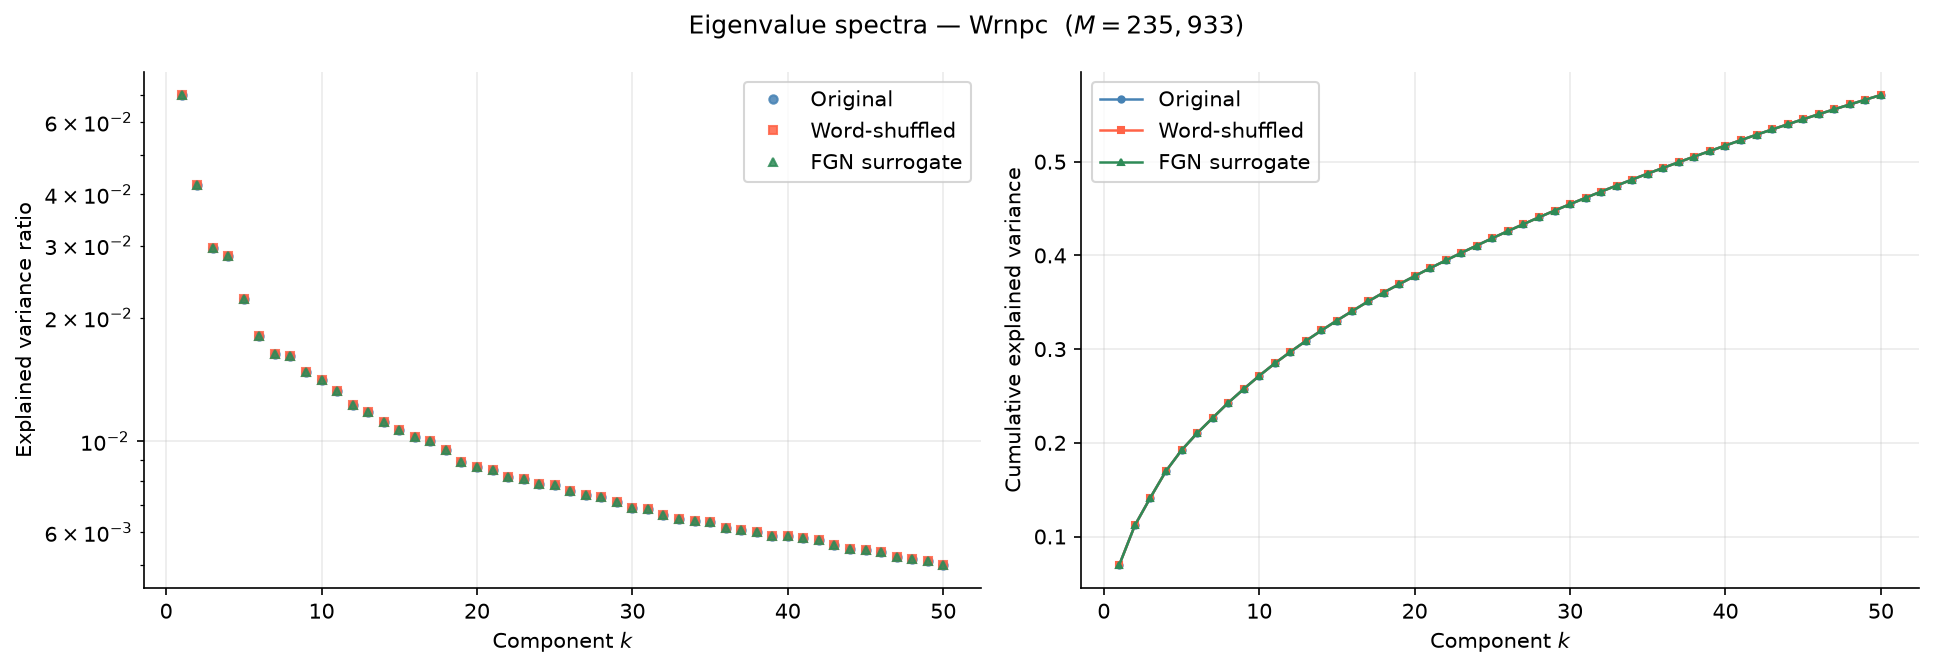
\includegraphics[width=\textwidth]{figures/eng_wrnpc/eng_wrnpc_02_spectra_comparison.png}
  \caption{Eigenvalue spectra and cumulative explained variance for
  \emph{War and Peace}. The three curves coincide: both surrogates are
  permutations of the original token sequence, so all three share the
  same covariance matrix and hence the same spectrum
  (Remark~\ref{rem:fgn_cov}). The figure therefore verifies the
  construction rather than reporting a comparison.}
  \label{fig:wrnpc_spectra}
\end{figure}

The semantic poles in Table~\ref{tab:wrnpc_pc} reveal two especially clear contrasts. PC2
separates military vocabulary (\emph{regiment}, \emph{infantry},
\emph{cavalry}, \emph{battalion}) from personal and emotional discourse
(\emph{really}, \emph{yourself}, \emph{feel}, \emph{understand}). PC3
contrasts physical action and embodied presence with philosophical and
moral reflection. PC1 partly reflects the known GloVe artefact in which
transliterated Russian names and emotionally inflected rare words lie
at the periphery of the embedding cloud; it is retained in the spectra
but interpreted cautiously.

\begin{table}[htbp]
\centering
\caption{Top-6 word types at the positive and negative poles of PC1,
PC2 and PC3 for \emph{War and Peace} ($R=100$, $F_{\min}=5$),
with frequencies in the filtered token sequence.
$B_k$ is a property of the component, not of the pole, and is therefore
shown once per pair; the largest value over the $K=20$ components is
shown in bold.}
\label{tab:wrnpc_pc}
\small
\setlength{\tabcolsep}{4pt}
\begin{tabular}{llr p{5.4cm} p{4.4cm}}
\toprule
PC & Pole & $B_k$ & Top words (freq) & Interpretation \\
\midrule
PC1 & $+$ & 1.643 &
  \emph{gerasim} (26), \emph{maidservant} (5), \emph{irritably} (6),
  \emph{piteously} (7), \emph{nikolaevich} (5), \emph{andreevich} (8)
  & Rare transliterated names and low-frequency emotive vocabulary
    (GloVe artefact) \\
PC1 & $-$ & &
  \emph{any} (465), \emph{government} (63), \emph{than} (533),
  \emph{its} (567), \emph{people} (557), \emph{us} (422)
  & High-frequency function words and abstract nouns (GloVe artefact) \\
\midrule
PC2 & $+$ & 1.855 &
  \emph{regiment} (226), \emph{infantry} (82), \emph{cavalry} (77),
  \emph{battalion} (44), \emph{squadron} (64), \emph{brigade} (5)
  & Military units and formations (War) \\
PC2 & $-$ & &
  \emph{really} (203), \emph{yourself} (117), \emph{feel} (133),
  \emph{myself} (148), \emph{laugh} (60), \emph{everybody} (118)
  & Personal and emotional discourse (Peace) \\
\midrule
PC3 & $+$ & \textbf{2.045} &
  \emph{walked} (70), \emph{sat} (345), \emph{feet} (112),
  \emph{yards} (20), \emph{screaming} (6), \emph{clutching} (12)
  & Physical action and embodied presence \\
PC3 & $-$ & &
  \emph{principles} (7), \emph{undertake} (10), \emph{renounce} (8),
  \emph{utmost} (12), \emph{justification} (11), \emph{obligations} (6)
  & Moral obligation and abstract reasoning \\
\bottomrule
\end{tabular}
\end{table}

\subsubsection{\emph{On the Origin of Species}}
\label{sec:darwin}



\emph{On the Origin of Species} contains $N=151{,}179$ raw tokens and
$M=58{,}913$ retained tokens, with $\alpha=0.771$ and
$\alpha_0=0.80$. PC1 explains $6.61\%$ of the variance, PC2
$3.58\%$, and the first ten components $26.4\%$. All three spectra
coincide, both surrogates being permutations of the original token
sequence (Figure~\ref{fig:darwin_spectra}).

PC1 is dominated by specialised nineteenth-century biological and
geological terminology at one pole and pronouns or conversational
markers at the other, and therefore contains a register-related
embedding artefact. PC2 is a substantive geographical-versus-epistemic
direction: spatial and biogeographical terms are opposed to the
language of inference and theoretical reasoning. PC3 contrasts
first-person field observations and concrete specimens with abstract
classification and synthesis. Table~\ref{tab:darwin_pc} also lists PC6,
the burstiest direction of this text.

\begin{table}[htbp]
\centering
\caption{Top-6 word types at the positive and negative poles of PC1,
PC2, PC3 and PC6 for \emph{On the Origin of Species} ($R=100$,
$F_{\min}=5$), with frequencies in the filtered token sequence.
PC4 and PC5 are omitted; PC6 is included because it carries the largest
burstiness of this text.
$B_k$ is a property of the component, not of the pole, and is therefore
shown once per pair; the largest value over the $K=20$ components is
shown in bold.}
\label{tab:darwin_pc}
\small
\setlength{\tabcolsep}{4pt}
\begin{tabular}{llr p{5.4cm} p{4.4cm}}
\toprule
PC & Pole & $B_k$ & Top words (freq) & Interpretation \\
\midrule
PC1 & $+$ & 1.255 &
  \emph{sessile} (11), \emph{faunas} (14), \emph{ovules} (6),
  \emph{plumage} (9), \emph{polymorphic} (9), \emph{insectivorous} (6)
  & Specialised 19th-c.\ natural history lexicon \\
PC1 & $-$ & &
  \emph{he} (163), \emph{him} (17), \emph{said} (47),
  \emph{us} (104), \emph{she} (24), \emph{his} (90)
  & Pronouns and interpersonal register (GloVe artefact) \\
\midrule
PC2 & $+$ & 1.888 &
  \emph{northern} (37), \emph{islands} (131), \emph{sea} (100),
  \emph{southern} (43), \emph{eastern} (13), \emph{island} (60)
  & Places and biogeographical setting \\
PC2 & $-$ & &
  \emph{innate} (7), \emph{slightest} (7), \emph{understand} (74),
  \emph{infer} (31), \emph{absolutely} (25), \emph{judgment} (12)
  & Scientific reasoning and theoretical inference \\
\midrule
PC3 & $+$ & 1.727 &
  \emph{me} (153), \emph{eat} (5), \emph{beaks} (10),
  \emph{squirrels} (5), \emph{legs} (37), \emph{rabbit} (5)
  & Field observations, specific specimens, first person \\
PC3 & $-$ & &
  \emph{geographical} (42), \emph{reduction} (5),
  \emph{proportional} (16), \emph{increased} (27),
  \emph{increase} (66), \emph{corresponding} (36)
  & Quantitative comparison and proportional reasoning \\
\midrule
PC6 & $+$ & \textbf{1.900} &
  \emph{seas} (13), \emph{arctic} (38), \emph{climate} (85),
  \emph{warmer} (12), \emph{deserts} (6), \emph{shores} (24)
  & Climate and physical environment (glacial-period chapters) \\
PC6 & $-$ & &
  \emph{character} (136), \emph{named} (12), \emph{female} (24),
  \emph{written} (7), \emph{characters} (170), \emph{original} (24)
  & Taxonomic description and nomenclature (partly register-driven) \\
\bottomrule
\end{tabular}
\end{table}

\subsubsection{\emph{Great Expectations}}
\label{sec:greatexp}

\emph{Great Expectations} contains $N=188{,}925$ raw tokens and
$M=64{,}410$ retained tokens, with $\alpha=0.689$ and
$\alpha_0=0.74$. PC1, PC2, and the first ten components account for
$6.54\%$, $4.34\%$, and $27.2\%$ of the variance, respectively. The
three covariance spectra are again coincident
(Figure~\ref{fig:greatexp_spectra}).

The positive pole of PC1 contains character names and Victorian
dialect, opposed to generic and abstract vocabulary, and is treated as
an embedding artefact. PC2 contrasts the spatial and kinetic language
of the river and the open country with introspective and conversational
language. PC3 opposes bodily action and gesture to a formal Latinate
register. The corresponding poles are listed in
Table~\ref{tab:greatexp_pc}.

\begin{table}[htbp]
\centering
\caption{Top-6 word types at the positive and negative poles
of PC1, PC2, and PC3 for \emph{Great Expectations}
($R=100$, $F_{\min}=5$).}
\label{tab:greatexp_pc}
\small
\setlength{\tabcolsep}{4pt}
\begin{tabular}{llr p{5.4cm} p{4.4cm}}
\toprule
PC & Pole & $B_k$ & Top words (freq) & Interpretation \\
\midrule
PC1 & $+$ & 1.228 &
  \emph{jaggers} (242), \emph{townsman} (6), \emph{stammered} (6),
  \emph{peeped} (5), \emph{biddy} (231), \emph{provis} (70)
  & Character names and Victorian dialect (GloVe artefact) \\
PC1 & $-$ & &
  \emph{will} (174), \emph{its} (151), \emph{government} (5),
  \emph{their} (175), \emph{any} (268), \emph{year} (25)
  & High-frequency generic and abstract vocabulary \\
\midrule
PC2 & $+$ & 1.209 &
  \emph{river} (59), \emph{near} (66), \emph{opened} (41),
  \emph{fell} (55), \emph{port} (7), \emph{yards} (9)
  & Spatial and kinetic language (river, marshes, forge) \\
PC2 & $-$ & &
  \emph{really} (41), \emph{understand} (53), \emph{think} (241),
  \emph{anybody} (30), \emph{myself} (235), \emph{yourself} (51)
  & Introspective and conversational register \\
\midrule
PC3 & $+$ & \textbf{1.244} &
  \emph{legs} (35), \emph{walked} (45), \emph{feet} (34),
  \emph{crying} (15), \emph{knees} (15), \emph{staring} (26)
  & Bodily action and gesture \\
PC3 & $-$ & &
  \emph{concerning} (13), \emph{expressly} (5), \emph{regarding} (8),
  \emph{relation} (12), \emph{undertake} (5), \emph{subordinate} (6)
  & Formal Latinate register \\
\bottomrule
\end{tabular}
\end{table}

\subsubsection{\emph{Ulysses}}
\label{sec:ulysses}

\emph{Ulysses} contains $N=264{,}165$ raw tokens and $M=101{,}489$
retained tokens, with $\alpha=0.763$ and $\alpha_0=0.80$. Its first
ten components account for $25.0\%$ of the variance, the smallest
fraction among the four texts, consistent with the diversity of
registers across its eighteen episodes
(Figure~\ref{fig:ulysses_spectra}).

PC1 is strongly affected by Dublin-specific proper names,
multilingual fragments, and neologisms. PC2 separates formal titles and
institutional naming from colloquial and intimate discourse. PC3
contrasts physical and material description with the vocabulary of
kinship, marriage and literary identity. These semantic poles are
listed in Table~\ref{tab:ulysses_pc}.

\begin{table}[htbp]
\centering
\caption{Top-6 word types at the positive and negative poles of PC1,
PC2 and PC3 for \emph{Ulysses} ($R=100$, $F_{\min}=5$), with
frequencies in the filtered token sequence.
$B_k$ is a property of the component, not of the pole, and is therefore
shown once per pair; the largest value over the $K=20$ components is
shown in bold.
A word type may appear at opposite poles of different components: the
components are orthogonal directions, not a partition of the
vocabulary.}
\label{tab:ulysses_pc}
\small
\setlength{\tabcolsep}{4pt}
\begin{tabular}{llr p{5.4cm} p{4.4cm}}
\toprule
PC & Pole & $B_k$ & Top words (freq) & Interpretation \\
\midrule
PC1 & $+$ & 1.286 &
  \emph{wonderworker} (6), \emph{dedalus} (174), \emph{maggy} (9),
  \emph{purefoy} (20), \emph{dignam} (83), \emph{voglio} (9)
  & Dublin proper names, neologisms and multilingual fragments
    (GloVe artefact) \\
PC1 & $-$ & &
  \emph{government} (14), \emph{any} (191), \emph{than} (169),
  \emph{people} (78), \emph{because} (219), \emph{year} (71)
  & Generic and institutional English (GloVe artefact) \\
\midrule
PC2 & $+$ & \textbf{1.495} &
  \emph{st} (6), \emph{william} (40), \emph{edward} (17),
  \emph{sir} (219), \emph{attended} (7), \emph{frederick} (10)
  & Formal titles and institutional naming \\
PC2 & $-$ & &
  \emph{yourself} (38), \emph{really} (49), \emph{feel} (104),
  \emph{stupid} (11), \emph{stuff} (24), \emph{ourselves} (10)
  & Colloquial and intimate register \\
\midrule
PC3 & $+$ & 1.329 &
  \emph{thick} (26), \emph{inches} (7), \emph{surface} (10),
  \emph{tail} (24), \emph{mud} (6), \emph{sloping} (9)
  & Physical and material description \\
PC3 & $-$ & &
  \emph{married} (56), \emph{marry} (10), \emph{poet} (29),
  \emph{sir} (219), \emph{son} (113), \emph{brother} (66)
  & Kinship, marriage and literary identity \\
\bottomrule
\end{tabular}
\end{table}

Taken together, the four texts show that PCA produces an ordered static
geometry whose leading directions are often semantically interpretable,
but whose first component can be contaminated by peripheral lexical
clusters. The temporal question is separate: whether visits along these
directions occur regularly or in concentrated textual episodes.

\FloatBarrier
\subsection{Burstiness across principal components}
\label{sec:component_burstiness_results}

We now turn from static geometry to temporal organisation. For each
component, threshold crossings define event sequences and IET
distributions. Figure~\ref{fig:burst_panel} and
Figures~\ref{fig:wrnpc_iet}, \ref{fig:darwin_iet}, \ref{fig:greatexp_iet}
and \ref{fig:ulysses_iet} show the representative-text evidence. In every text, the original
series has broader IET distributions and larger $B_k$ than either
control. The spectra are component dependent and generally largest
among the early PCs, but the decay with component rank is not monotone.
This non-monotonicity is expected because PCA orders variance rather
than burstiness.

\subsubsection{\emph{War and Peace}}

For PC1--PC3, the original IET distributions extend well beyond the
geometric reference, whereas the shuffled and FGN controls closely
follow it (Figure~\ref{fig:wrnpc_iet}). The burstiness spectrum in
Figure~\ref{fig:burst_panel}A is above both controls for all 20
components. PC3 has the largest value, $B_3=2.045$, approximately $2.1$ times the
geometric baseline and more than twice the corresponding null values
($B_3^{\rm surr}=0.976$, $B_3^{\rm FGN}=0.974$). Because events are
threshold crossings of the upper tail, this measures the clustering of
the positive pole of PC3: passages of physical action and embodied
movement, which are concentrated in the battle and campaign chapters.
The eigenvalue--burstiness correlation is positive but imperfect,
$r=0.702$ ($P=0.0055$).

\begin{figure}[htbp]
  \centering
  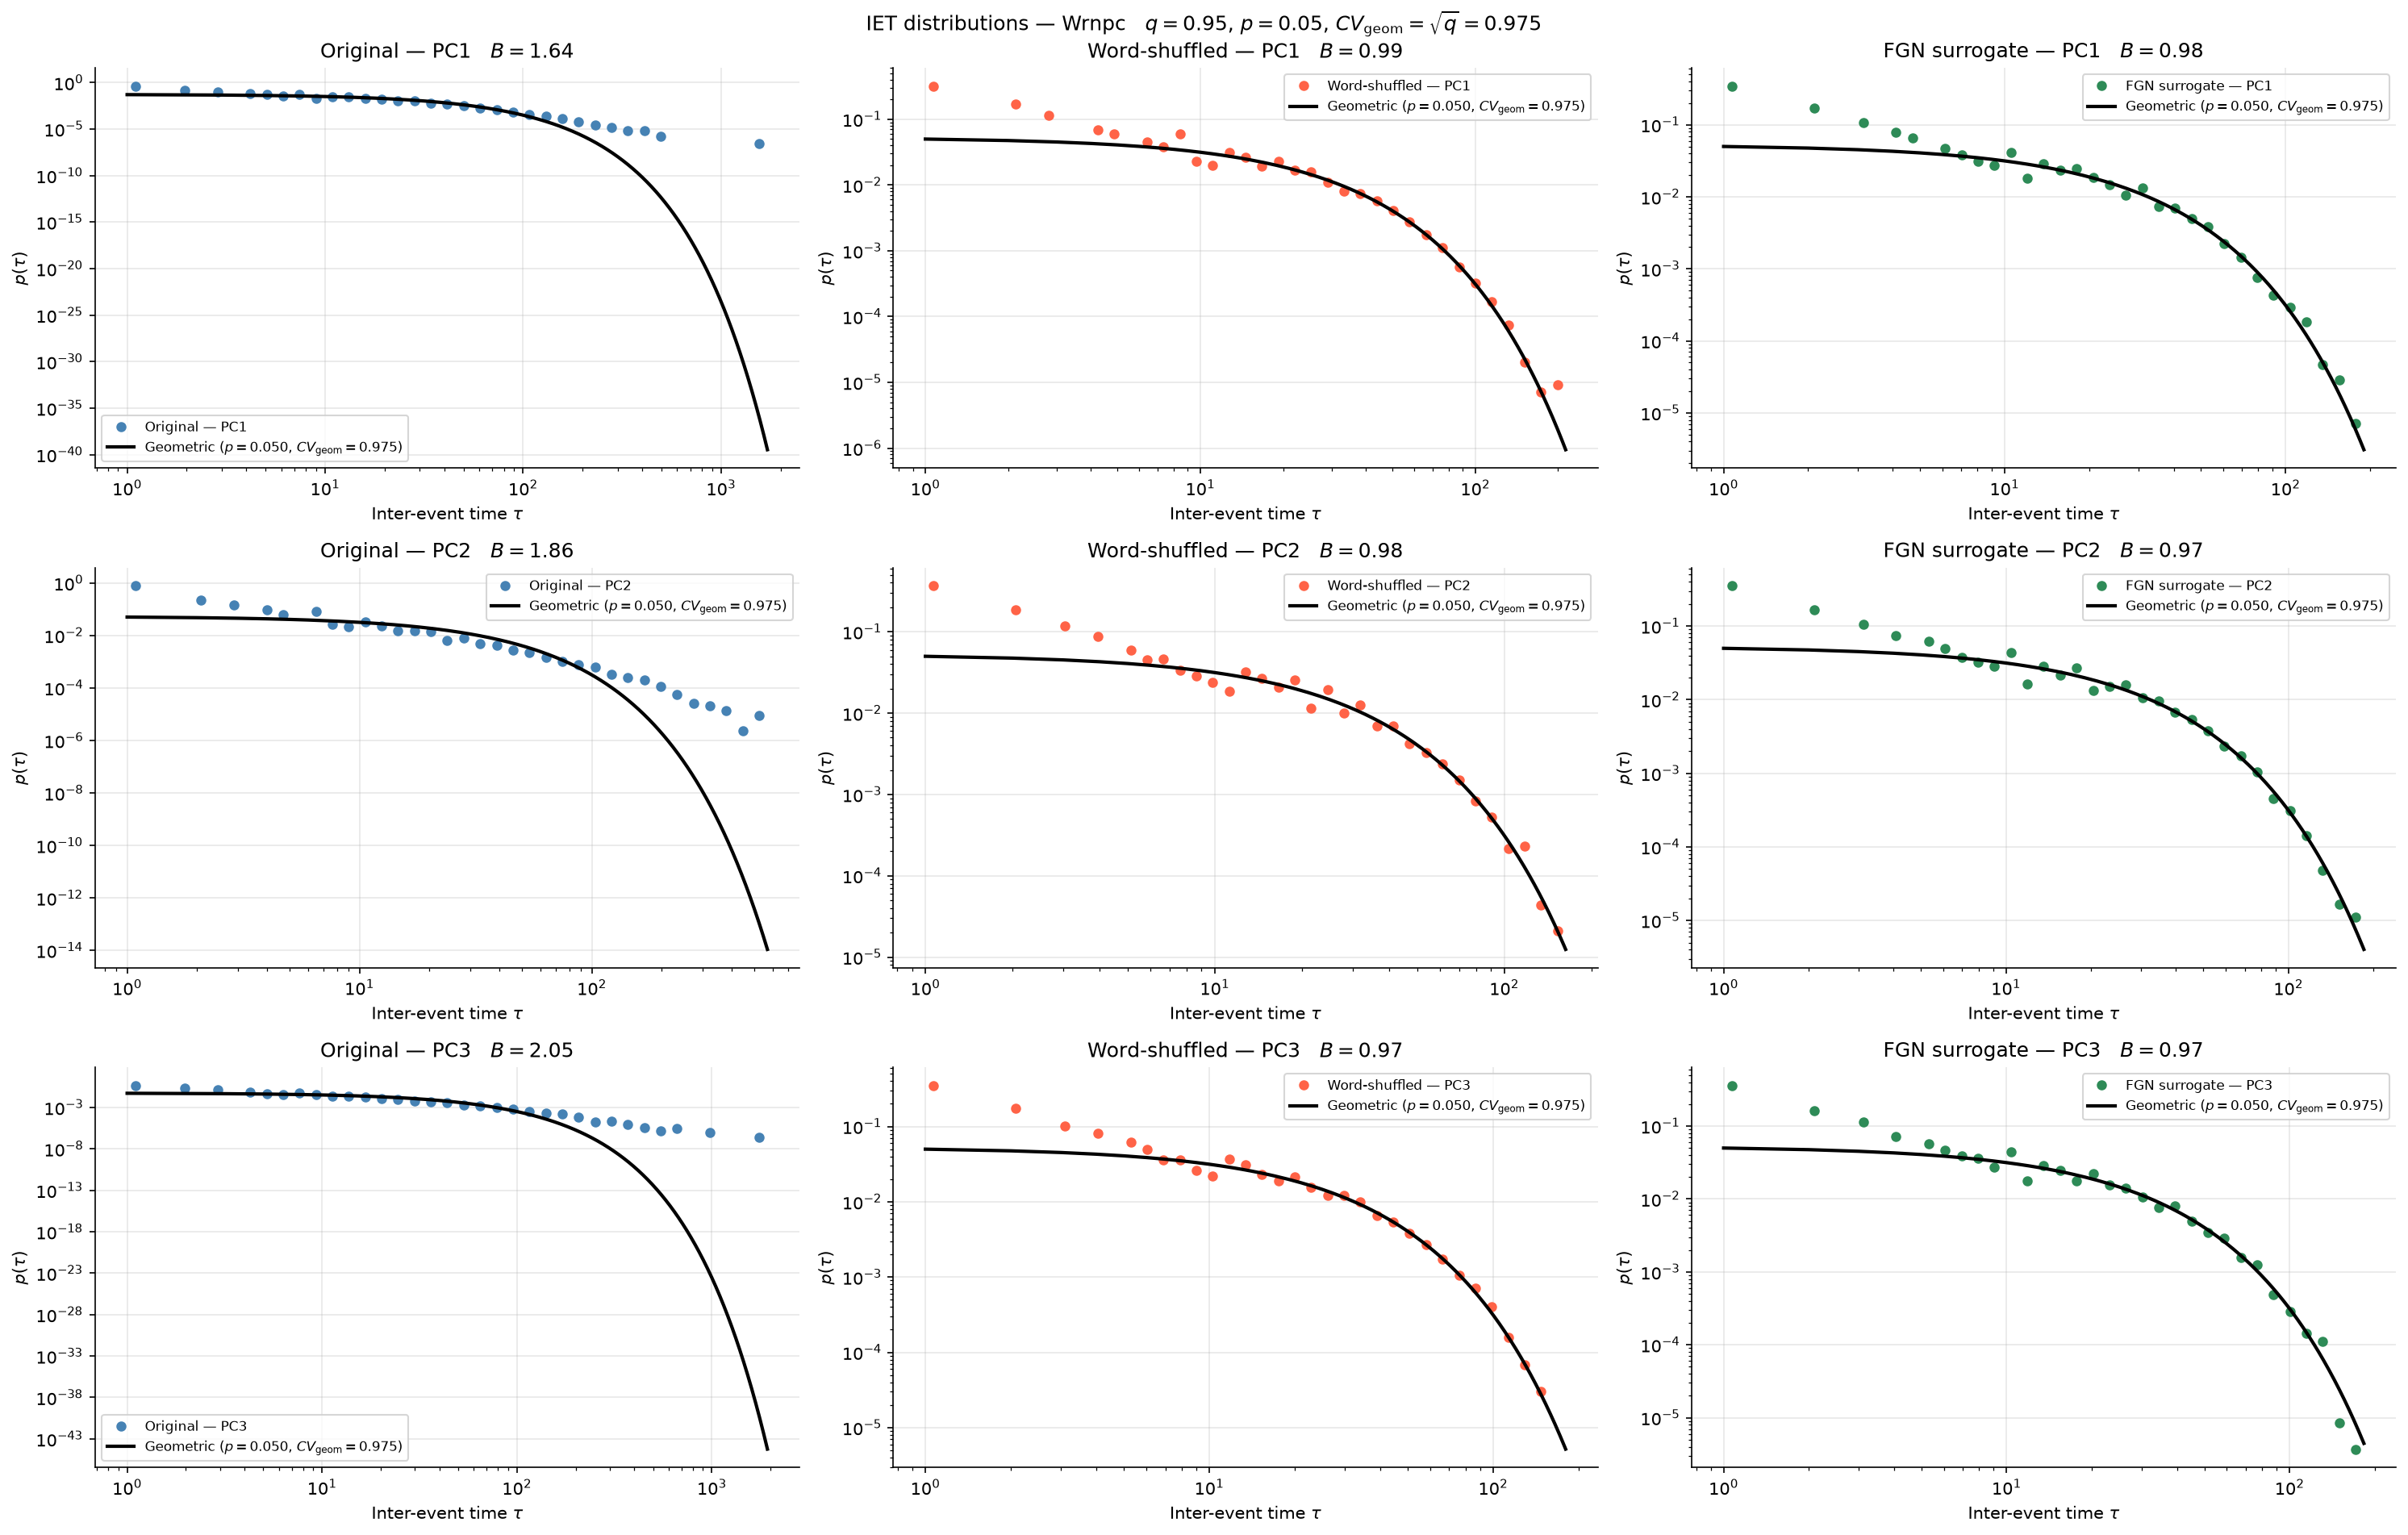
\includegraphics[width=\textwidth]{figures/eng_wrnpc/eng_wrnpc_03_iet_comparison.png}
  \caption{Inter-event-time distributions for PC1--PC3 of
  \emph{War and Peace} at $q=0.95$. Columns show the original text
  (blue), word-shuffled null (red), and FGN surrogate (green). The
  original projections have broad tails, whereas both controls lie
  close to the geometric reference.}
  \label{fig:wrnpc_iet}
\end{figure}

\begin{figure}[htbp]
  \centering
  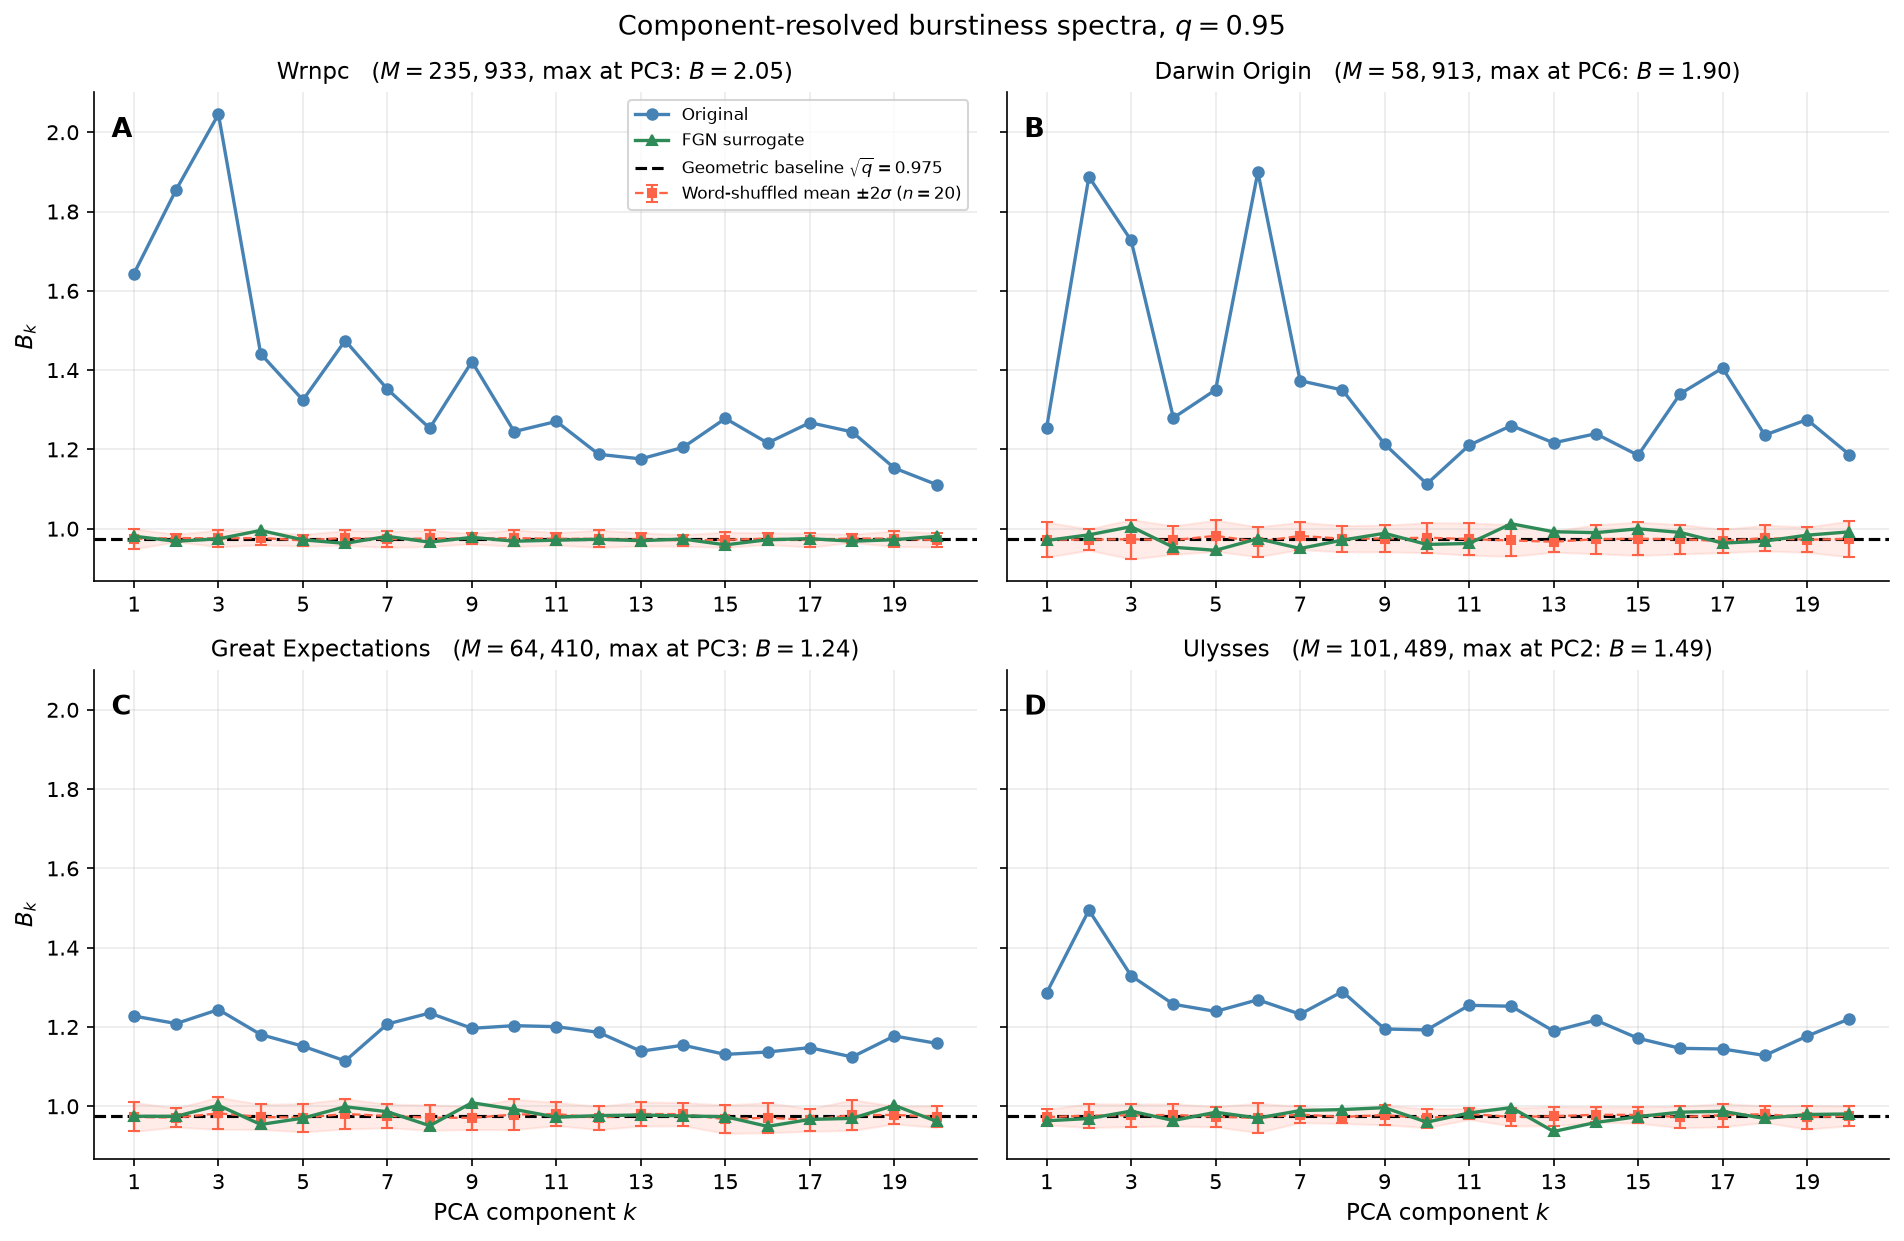
\includegraphics[width=\textwidth]{figures/panel_burstiness_spectra.png}
 \caption{Component-resolved burstiness spectra at $q=0.95$ for the four
  representative texts: \textbf{A} \emph{War and Peace},
  \textbf{B} \emph{On the Origin of Species},
  \textbf{C} \emph{Great Expectations}, \textbf{D} \emph{Ulysses}.
  In every panel the original (blue circles) lies above the FGN surrogate
  (green triangles), the word-shuffled mean$\pm2\sigma$ band over 20
  realisations (red), and the geometric baseline
  $\CV_{\rm geom}=\sqrt{q}\simeq0.975$, for all 20 components.
  Events are crossings of the upper tail, so $B_k$ measures the
  clustering of visits to the \emph{positive} pole of each component
  (Tables~\ref{tab:wrnpc_pc}--\ref{tab:ulysses_pc}).
  Burstiness is not monotone in PCA rank, because PCA orders components
  by variance rather than by temporal clustering: the maximum falls at
  PC3, PC6, PC3 and PC2 respectively, and never at PC1 --- although in
  \textbf{B} and \textbf{C} the leading values are closely spaced.}
  \label{fig:burst_panel}
\end{figure}


\subsubsection{\emph{On the Origin of Species}}

The original projections have broad IET tails, particularly for PC2 and
PC3, while both controls remain close to geometric
(Figure~\ref{fig:darwin_iet}). Burstiness is high across the leading
directions but peaks away from the leading eigenvalue: the two largest
values, $B_6=1.900$ and $B_2=1.888$, differ by less than one per cent
and are followed by $B_3=1.727$, while PC1 is markedly lower at
$B_1=1.255$. Both PC6 and PC2 have positive poles tied to specific
parts of the book --- climate and the glacial period, and places and
biogeography respectively (Table~\ref{tab:darwin_pc}) --- which is what
concentrates their threshold crossings. The full
original-over-control ordering holds for all 20 components. The linear
eigenvalue--burstiness correlation is weak, $r=0.295$ ($P=0.169$),
while the rank correlation is moderate, $\rho=0.460$ ($P=0.042$): the
association is monotone but not linear. That the burstiness maximum
lies well away from PC1 states the point without recourse to any
correlation measure --- the direction of greatest semantic variance is
not the direction of greatest temporal clustering.

\subsubsection{\emph{Great Expectations}}

The original PC1--PC3 IET distributions again have broader tails than
the controls (Figure~\ref{fig:greatexp_iet}). At $q=0.95$,
$B_1=1.228$, $B_2=1.209$ and $B_3=1.244$, while the null values lie in
$0.95$--$1.01$. The original remains above both controls over all 20
components (Figure~\ref{fig:burst_panel}C), but the spectrum is flatter
and lower overall than for \emph{War and Peace}: the largest value
exceeds $B_1$ by only $1.3\%$, against $25\%$ in Tolstoy, and the mean
over the twenty components, $1.18$, is the lowest of the four texts.
Component-level burstiness is therefore present throughout the spectrum
without being concentrated in any particular direction. The
eigenvalue--burstiness correlation is $r=0.511$ ($P=0.014$), with a
rank correlation $\rho=0.579$ ($P=0.009$).



\subsubsection{\emph{Ulysses}}

For \emph{Ulysses}, the original IET distributions are broad for all
three displayed components, while both controls collapse towards the
geometric reference (Figure~\ref{fig:ulysses_iet}). The spectrum peaks
at PC2, $B_2=1.495$, with $B_1=1.286$ and $B_3=1.329$
(Figure~\ref{fig:burst_panel}D); the positive pole of PC2 is the
register of formal titles and institutional naming
(Table~\ref{tab:ulysses_pc}), which the novel deploys in concentrated
parodic passages rather than evenly. The original exceeds both controls
throughout the first 20 components. Here the two correlation measures
diverge most strongly: $r=0.571$ ($P=0.041$) against $\rho=0.817$
($P<10^{-4}$), so that the association between semantic variance and
burstiness is close to monotone while being poorly described by a
linear fit.

Averaged over the first 20 components at $q=0.95$, the representative
texts have $\bar B^{\rm orig}$ of $1.36$ (\emph{War and Peace}),
$1.35$ (\emph{On the Origin of Species}), $1.23$ (\emph{Ulysses}) and
$1.18$ (\emph{Great Expectations}), against $\bar B\simeq0.97$--$0.98$
for both null models in every case. The ordering is not a simple
function of either text length or rank-sequence DFA exponent.
The common feature is that component-level burstiness is present in the
original semantic trajectories and absent from both null models.

\FloatBarrier
\subsection{Robustness to the threshold quantile and to the number of
components}
\label{sec:single_text_robustness}

The component separation is not tied to the default $q=0.95$.
Figure~\ref{fig:sweep_panel} shows the mean
burstiness over $k=1,\ldots,20$ as $q$ varies from $0.60$ to $0.99$;
the corpus-level version of the ordering fraction is given in
Section~\ref{sec:corpus_robustness}.
For each of the four representative texts, the ordering holds for all
20 components throughout the displayed range. As expected, the
absolute burstiness increases towards more extreme thresholds because
rare visits to the upper tail accentuate episode-to-episode clustering.

\begin{figure}[htbp]
  \centering
  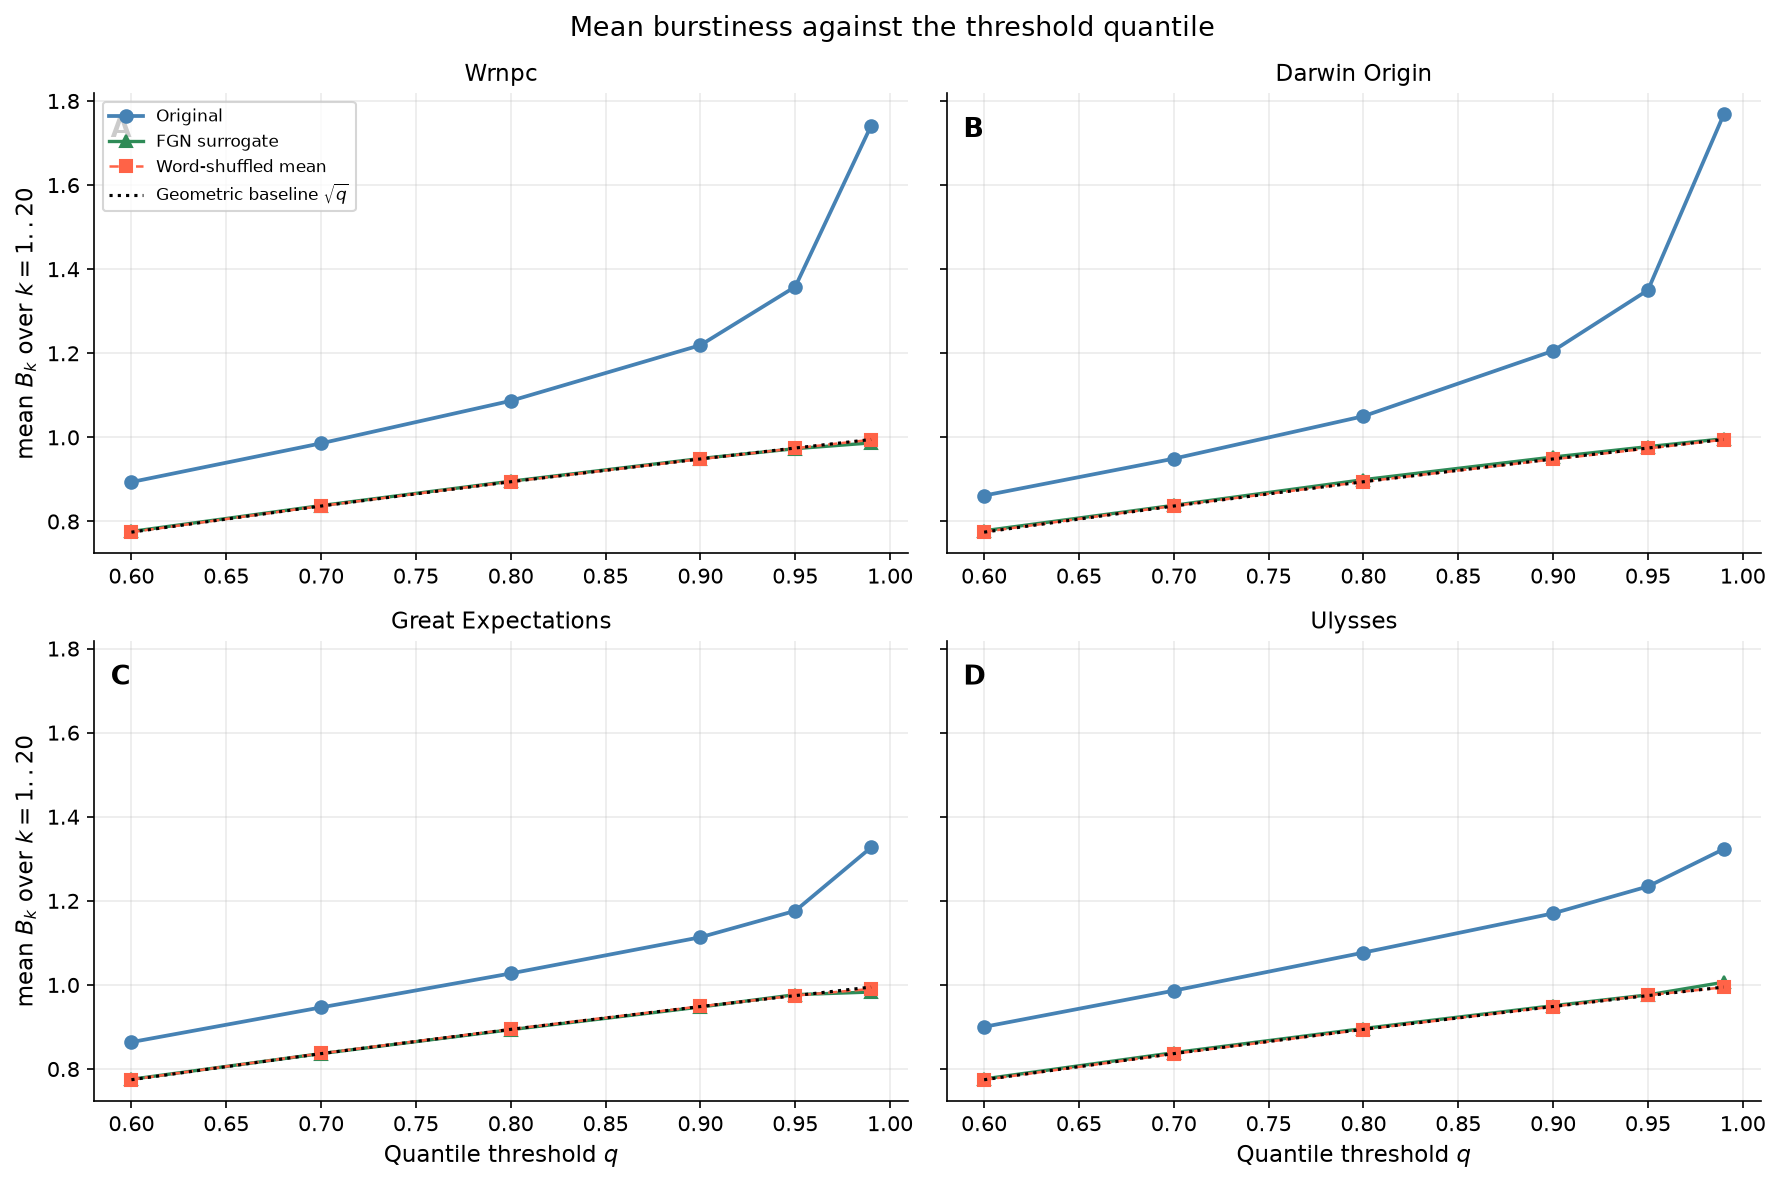
\includegraphics[width=\textwidth]{figures/panel_quantile_sweep.png}
  \caption{Mean burstiness over $k=1,\ldots,20$ as a function of the
  threshold quantile $q$, for the four representative texts:
  \textbf{A} \emph{War and Peace}, \textbf{B} \emph{On the Origin of
  Species}, \textbf{C} \emph{Great Expectations}, \textbf{D}
  \emph{Ulysses}. The original stays above both controls and above the
  geometric baseline $\sqrt{q}$ throughout $q \in [0.60, 0.99]$, and the
  full ordering $B_k^{\rm orig} > B_k^{\rm FGN}$ and
  $B_k^{\rm orig} > B_k^{\rm surr}$ holds for all 20 components at every
  displayed $q$ in each text. Absolute burstiness grows towards more
  extreme thresholds, as rare visits to the upper tail accentuate
  episode-to-episode clustering.}
  \label{fig:sweep_panel}
\end{figure}

The separation is likewise not an artefact of truncating the spectrum at
$K=20$. 
The retained components account for $35$--$38\%$ of the embedding
variance; refitting the PCA with $K=50$ and recomputing the spectrum at
$q=0.95$ leaves every component above the independent-event baseline in
all four texts, with a minimum of $B_k=1.041$, some $7\%$ above
$\CV_{\rm geom}$. Burstiness does decline with component index: the mean
falls from $1.18$--$1.36$ over the first twenty components to
$1.11$--$1.19$ over components $21$--$50$, while the variance carried per
component falls from $1.9\%$ to $0.65\%$. 
The choice $K=20$ is conventional rather than principled; what the
extension to $K=50$ shows is that it does not act as a threshold beyond
which component-level burstiness disappears. The leading components are
also the ones for which the semantic poles were examined
(Section~\ref{sec:semantic_geometry_results}).

\FloatBarrier
\section{Corpus-level generalisation}
\label{sec:corpus}

Having established the component-resolved pattern in four
representative texts (Section~\ref{sec:oliver}), we now assess its
generality across the full corpus.
%
%\NOTE{All computations use local PCA (eigenvectors re-estimated per
%text), GloVe-300 embeddings, frequency filter $R=100$, hapax filter
%$F_{\min}=5$, $N_{\rm surr}=10$ word-shuffled realisations,
%and a single FGN realisation per text (seed 42).
%Default quantile $q=0.95$ unless stated.}

\subsection{Corpus description}
\label{sec:corpus_texts}

The corpus comprises 16 English literary texts from Project Gutenberg,
sspanning novels, scientific treatises and travel writing, in English editions 
and translations published between the eighteenth and early twentieth centuries.
(Table~\ref{tab:corpus}).
Raw token counts range from approximately $56{,}000$ (The Picture of
Dorian Gray) to $565{,}000$ (War and Peace), with filtered token counts
$M$ (after high-frequency and hapax removal, OOV excluded) between
$17{,}000$ and $236{,}000$.
DFA scaling exponents $\alpha$ lie in the range $[0.63, 0.85]$,
consistent with the literature on long-range correlations in English
texts \citep{Ebeling1995, MontemurroPury2002}.


\begin{table}[t]
\centering
\caption{Corpus of 16 literary and scientific texts.
$N$: total token count after tokenisation.
$M$: content tokens after frequency filtering
(top $R=100$ words removed, minimum frequency~5).
$\alpha$: DFA scaling exponent of the rank sequence.
$\alpha_0$: FGN generator exponent matched to $\alpha$ (bisection
tolerance $0.01$).}
\label{tab:corpus}
\small
\begin{tabular}{llrrll}
\toprule
Title & Author & $N$ & $M$ & $\alpha$ & $\alpha_0$ \\
\midrule
Pride and Prejudice        & Austen    & 122{,}226 &  42{,}364 & 0.642 & 0.67 \\
Don Quixote (transl.)      & Cervantes & 403{,}152 & 147{,}279 & 0.711 & 0.76 \\
On the Origin of Species   & Darwin    & 151{,}179 &  58{,}913 & 0.770 & 0.80 \\
The Voyage of the Beagle   & Darwin    & 206{,}728 &  84{,}931 & 0.629 & 0.67 \\
David Copperfield          & Dickens   & 363{,}557 & 134{,}409 & 0.727 & 0.78 \\
Great Expectations         & Dickens   & 188{,}925 &  64{,}410 & 0.689 & 0.73 \\
Oliver Twist               & Dickens   & 161{,}529 &  59{,}729 & 0.711 & 0.76 \\
Ulysses                    & Joyce     & 264{,}165 & 101{,}489 & 0.763 & 0.80 \\
The Jungle Book            & Kipling   & 151{,}161 &  49{,}522 & 0.775 & 0.83 \\
Moby Dick                  & Melville  & 215{,}652 &  82{,}773 & 0.694 & 0.73 \\
Principia Mathematica      & Newton    & 112{,}225 &  26{,}347 & 0.815 & 0.85 \\
The Analysis of Mind       & Russell   &  88{,}342 &  30{,}449 & 0.743 & 0.76 \\
War and Peace              & Tolstoy   & 564{,}788 & 235{,}933 & 0.721 & 0.76 \\
Huckleberry Finn           & Twain     & 145{,}924 &  52{,}741 & 0.774 & 0.83 \\
Tom Sawyer                 & Twain     &  71{,}102 &  22{,}085 & 0.788 & 0.80 \\
The Picture of Dorian Gray & Wilde     &  55{,}619 &  16{,}776 & 0.845 & 0.87 \\
\bottomrule
\end{tabular}
\end{table}

\begin{quote}
Per-text IET distributions and burstiness spectra for all texts and
threshold values can be regenerated with \texttt{scripts/run\_text.py}
in the code repository. The main text reports the aggregated corpus
results.
\end{quote}


% ??????????????????????????????????????????????????????????
% Corpus ordering subsections ? rewritten
% ??????????????????????????????????????????????????????????

\subsection{Component-resolved burstiness holds corpus-wide}
\label{sec:corpus_ordering}

The corpus-level component spectrum is summarised in
Figure~\ref{fig:corpus_spectrum}.
Averaging the burstiness spectrum $\{\bk\}$ across all 16 texts
at quantile $q = 0.95$, the original texts are systematically more
bursty than both null models across all 20 PCA components:
$\langle B_k^{\rm orig}\rangle_{\rm texts} \in [1.16, 1.54]$
(mean $1.26$), while both null models cluster tightly around
the geometric baseline $\CV_{\rm geom} = \sqrt{0.95} \approx 0.975$:
$\langle B_k^{\rm surr}\rangle \in [0.973, 0.978]$ and
$\langle B_k^{\rm FGN}\rangle \in [0.958, 0.983]$.

At the level of individual $({\rm text}, k)$ pairs
($16 \times 20 = 320$ pairs):
\begin{itemize}
  \item $B_k^{\rm orig} > B_k^{\rm surr}$ in $\mathbf{100\%}$ of pairs.
  \item $B_k^{\rm orig} > B_k^{\rm FGN}$ in $\mathbf{100\%}$ of pairs.
  \item $|B_k^{\rm FGN}/B_k^{\rm surr} - 1| < 0.05$ in
        $\mathbf{95.6\%}$ of pairs.
\end{itemize}

The appropriate summary statistic for the magnitude of the effect
is the \emph{per-text mean ratio}, computed by averaging
$B_k^{\rm orig}/B_k^{\rm surr}$ over the 20 components for each
text and then averaging over the 16 texts:
\begin{equation}
  \left\langle \frac{B_k^{\rm orig}}{B_k^{\rm surr}}
  \right\rangle_{\rm texts}
  \;=\; 1.29 \;\pm\; 0.03,
  \qquad t = 8.7,\quad P < 10^{-6},
  \label{eq:ratio_corpus}
\end{equation}
where $\pm$ denotes the standard error of the mean over 16 texts.
The original texts are thus on average $\sim 30\%$ more bursty
than the word-shuffled null, which itself sits at the geometric baseline.
 The per-text values range from $1.17$ (\emph{Pride and Prejudice}) to
$1.73$ (\emph{Principia Mathematica}), with a spread across texts
(sd $= 0.13$) that is uncorrelated with text length
($r=-0.04$ against $M$). The four expository texts of the corpus
occupy four of the five highest positions (mean $1.45$ against $1.24$
for the twelve narrative works), which is consistent with the
chapter-level topical segmentation of expository prose; with four
non-fiction texts this is an observation to be tested on a larger and
deliberately balanced corpus, not a result.
The analogous ratio for the FGN surrogate is
$\langle B_k^{\rm orig}/B_k^{\rm FGN}\rangle = 1.29 \pm 0.03$,
indistinguishable from the word-shuffled value.

The two null models satisfy
$\langle B_k^{\rm FGN}/B_k^{\rm surr}\rangle = 1.001 \pm 0.001$
(range over texts $[0.996, 1.005]$; $t = 1.1$, $P = 0.28$):
the FGN surrogate and the word-shuffled null are statistically
indistinguishable at the corpus level
(Section~\ref{sec:corpus_diffs}).

\begin{figure}[htbp]
  \centering
  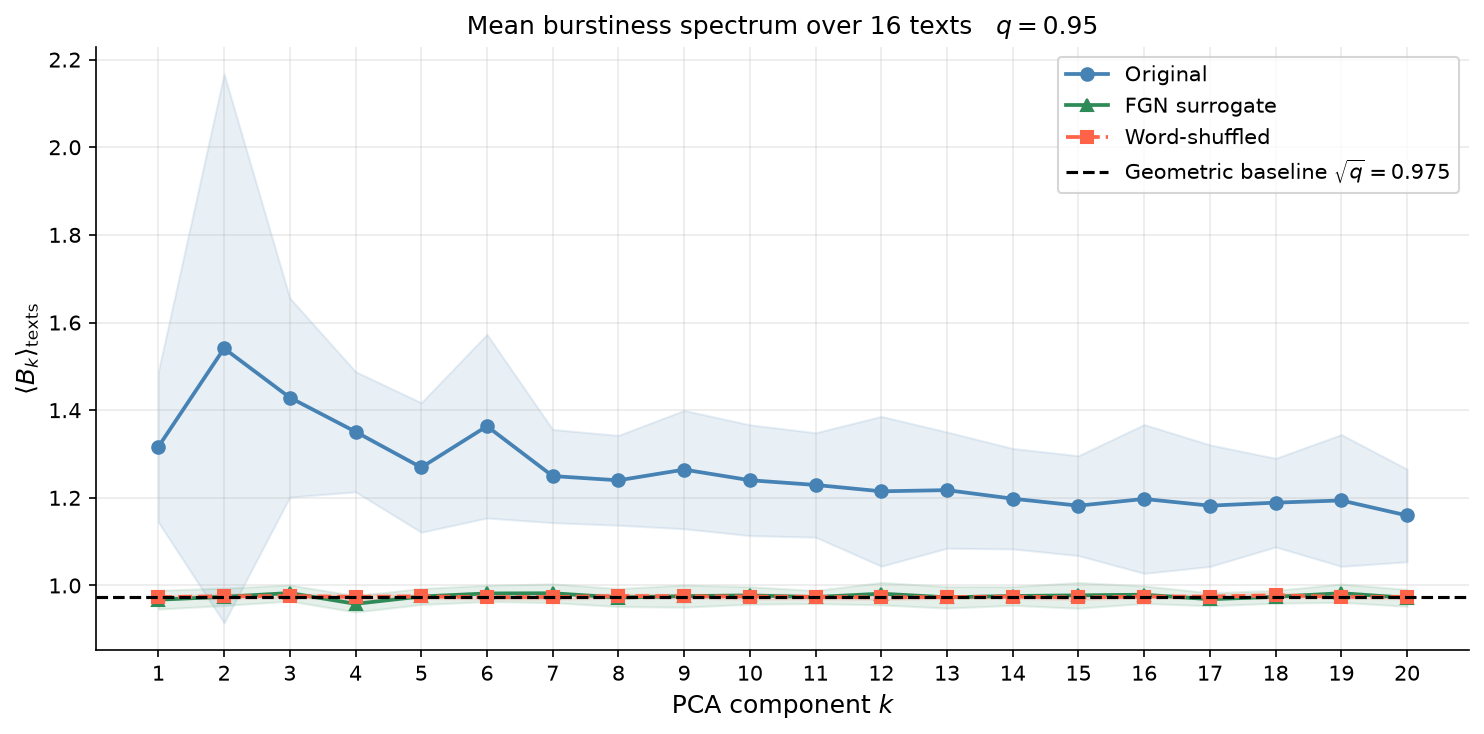
\includegraphics[width=\textwidth]{figures/fig1_mean_spectrum.png}
  \caption{Mean component-resolved burstiness spectrum across the
  analysed corpus at $q=0.95$. Curves show the mean $\langle B_k\rangle$
  over texts for $k=1,\ldots,20$; shaded bands indicate one standard
  deviation. The original texts (blue) are above the FGN surrogate
  (green), word-shuffled null (red), and geometric baseline
  $\sqrt{q}\simeq0.975$ at every component. The largest corpus means
  occur among the early components, followed by a broad decline with
  non-monotone secondary peaks.}
  \label{fig:corpus_spectrum}
\end{figure}


\subsection{Robustness to the threshold quantile}
\label{sec:corpus_robustness}

Figure~\ref{fig:corpus_robustness} shows the fraction of
$({\rm text}, k)$ pairs satisfying the ordering conditions as a
function of $q \in \{0.60, 0.70, 0.80, 0.90, 0.95, 0.99\}$.

The full ordering $B_k^{\rm orig} > B_k^{\rm surr}$ and
$B_k^{\rm orig} > B_k^{\rm FGN}$ is satisfied in $100\%$
of pairs for all $q \in [0.60, 0.95]$, and in $98.1\%$ of pairs at the
extreme $q = 0.99$.
The null-model indistinguishability criterion
$|B_k^{\rm FGN}/B_k^{\rm surr} - 1| < 0.05$ is met by $\geq 99\%$ of
pairs for $q \leq 0.90$, by $96\%$ at $q = 0.95$, and decreases to
$73\%$ at $q = 0.99$.

This degradation at the extreme threshold is expected: at the corpus
median, $M \approx 59{,}000$, the event rate $p = 0.01$ leaves only
$\sim 590$ events per series, giving a relative error on the IET
estimator of $\sim 4\%$, rising to $\sim 8\%$ for the shortest text
($M = 16{,}776$) --- comparable to or larger than the magnitude of
$B^{\rm FGN} - B^{\rm surr}$ at this threshold.
For $q = 0.95$ the same texts give $\sim 3{,}000$ and $\sim 840$ events,
with relative errors of $1.8\%$ and $3.5\%$, well within the regime
where the null-model comparison is reliable.

The same estimator noise accounts for the six pairs out of 320 that fail the full ordering at $q=0.99$.

\begin{figure}[htbp]
  \centering
  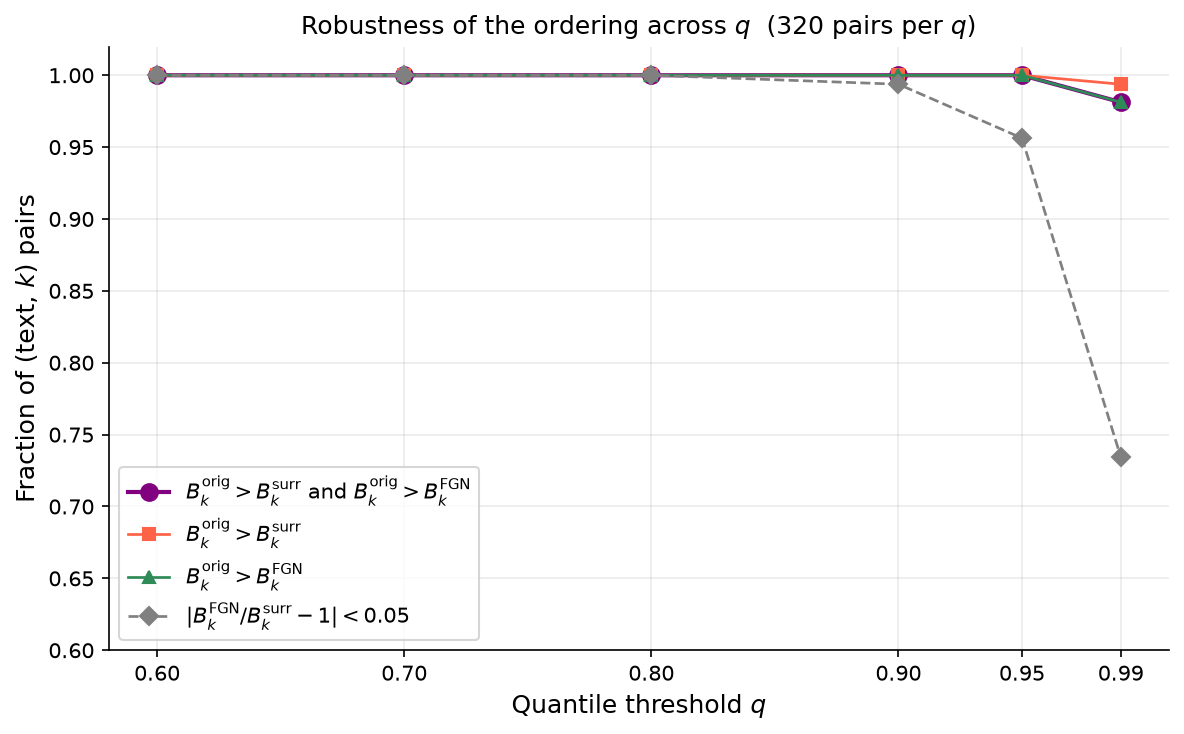
\includegraphics[width=0.72\textwidth]{figures/fig2_robustness_vs_q.png}
  \caption{%
    \textbf{Robustness of the burstiness ordering across quantile
    threshold $q$.}
    Each point: fraction of $({\rm text}, k)$ pairs ($320$ per $q$)
    satisfying the indicated condition.
    Purple circles: full ordering
    $B_k^{\rm orig} > B_k^{\rm surr}$ and $B_k^{\rm orig} >
    B_k^{\rm FGN}$.
    Red squares: $B_k^{\rm orig} > B_k^{\rm surr}$.
    Green triangles: $B_k^{\rm orig} > B_k^{\rm FGN}$.
    Grey diamonds: $|B_k^{\rm FGN}/B_k^{\rm surr} - 1| < 0.05$.
    The ordering is robust for $q \in [0.60, 0.95]$; the slight
    degradation at $q = 0.99$ is due to estimator noise at
    $p = 0.01$.
  }
  \label{fig:corpus_robustness}
\end{figure}


\subsection{Distribution of burstiness ratios}
\label{sec:corpus_diffs}

Figure~\ref{fig:corpus_diffs} shows the distribution of the ratios
$B^{\rm orig}/B^{\rm surr}$, $B^{\rm orig}/B^{\rm FGN}$, and
$B^{\rm FGN}/B^{\rm surr}$ over all 320 $({\rm text}, k)$ pairs
at $q = 0.95$.

Panel~A shows that both orig--null ratios are concentrate
well above 1, with no mass below 1.
The two distributions (orig/surr and orig/FGN) are nearly
identical in shape and location, confirming that the FGN and
word-shuffled null models are equally poor surrogates for the
original burstiness.


Panel~B isolates the ratio $B^{\rm FGN}/B^{\rm surr}$, which is tightly
concentrated around 1 over the 320 pairs (mean $1.0008$, sd $0.022$,
range $[0.91, 1.09]$). Because components within a text are not
independent, the test is performed on the 16 per-text means: a
one-sample $t$-test against unity gives $t = 1.13$, $P = 0.28$. The two
null models are statistically indistinguishable, and the distribution
is symmetric with no indication of a directional bias.

Together, Figures~\ref{fig:corpus_spectrum}--\ref{fig:corpus_diffs}
establish the corpus-level result:
\begin{equation}
  B_k^{\rm orig} \;\gg\; B_k^{\rm FGN} \;\approx\; B_k^{\rm surr}
  \qquad \forall\, k,\; \forall\, \text{text in corpus},
  \label{eq:ordering_corpus}
\end{equation}
with a mean excess of the original over the word-shuffled null of
$\sim 30\%$. The ordering holds for every text and every component
irrespective of length, genre, DFA exponent and choice of quantile
threshold; its magnitude, by contrast, varies systematically between
texts (Section~\ref{sec:corpus_ordering}).



\begin{figure}[htbp]
  \centering
  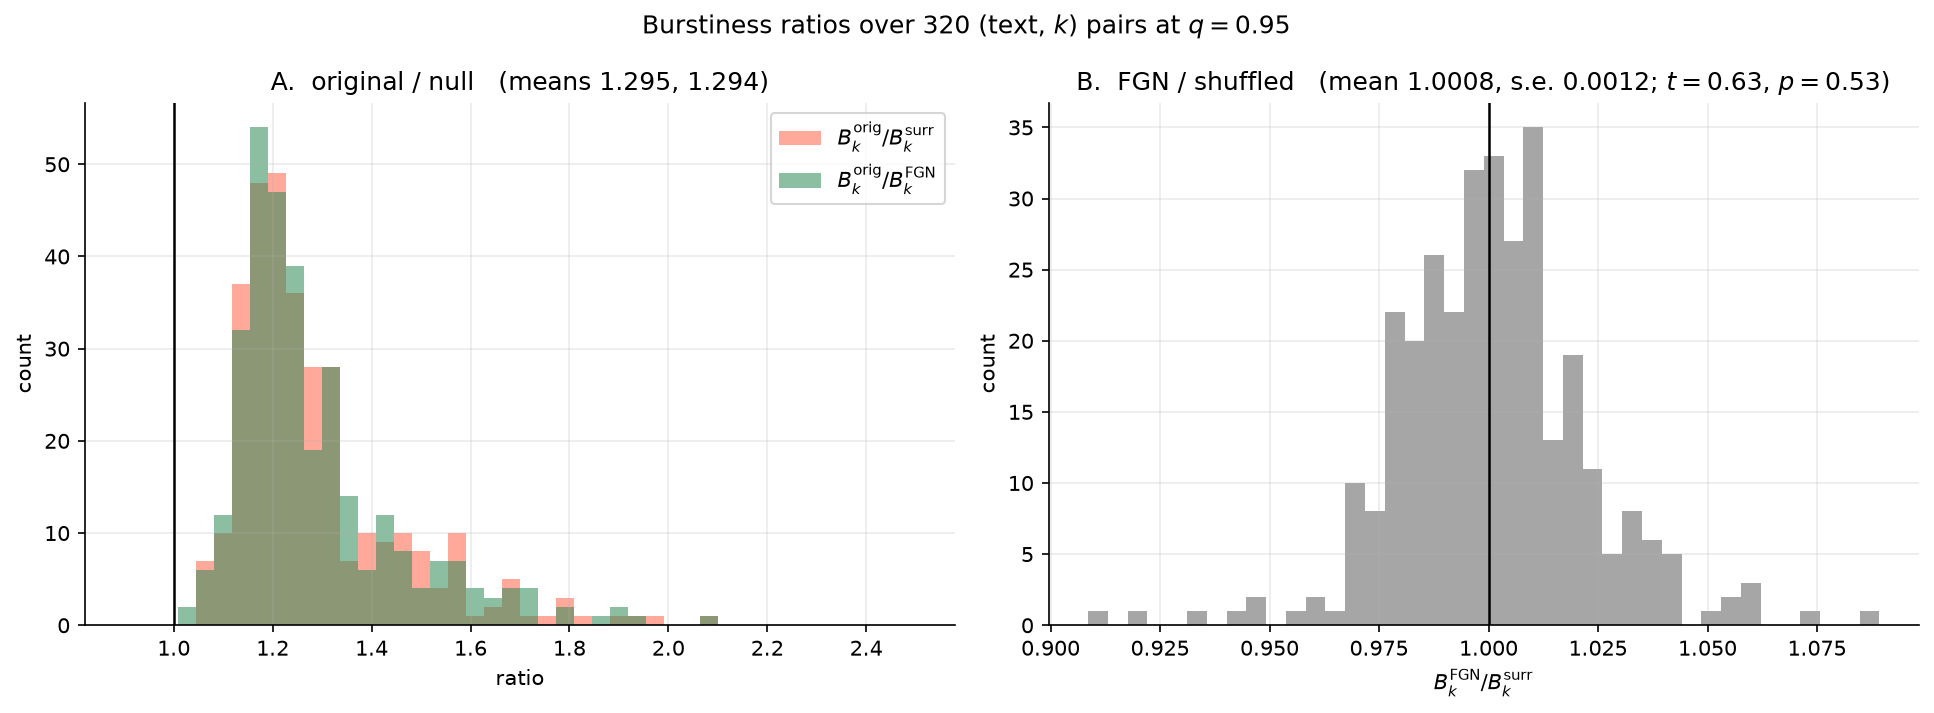
\includegraphics[width=\textwidth]{figures/fig3_difference_distributions.png}
  \caption{%
    \textbf{Distribution of burstiness ratios over
    320 (text, $k$) pairs at $q = 0.95$.}
    \textbf{Panel A}: distributions of $B_k^{\rm orig}/B_k^{\rm surr}$
    (red) and $B_k^{\rm orig}/B_k^{\rm FGN}$ (green), both
    concentrated well above 1.
    The two distributions are nearly identical, confirming that the
    two null models are equivalently far below the original.
    \textbf{Panel B}: distribution of $B_k^{\rm FGN}/B_k^{\rm surr}$,
    tightly centred on 1 (mean $1.0008$, s.e.\ $0.0012$;
    $t = 0.63$, $P = 0.53$), statistically indistinguishable from
    unity, confirming
    $B_k^{\rm FGN} \approx B_k^{\rm surr}$ across the entire corpus.
  }
  \label{fig:corpus_diffs}
\end{figure}

\FloatBarrier
% ------------------------------------------------------------
\section{Temporal persistence in semantic projection space}
\label{sec:entropy}

Sections~\ref{sec:oliver} and~\ref{sec:corpus} establish that the
original semantic trajectories have elevated component-resolved
burstiness and are separated from both controls. We now test the same
temporal organisation in the continuous projections using normalised
autocorrelation functions and DFA. An information-theoretic argument
explains why the long-range correlations imposed on the FGN rank
sequence need not survive the mapping into embedding space.


% ============================================================
% NOTE TO CO-AUTHOR (M.DE.) --- Sec. "Conditional entropy": decide
% whether to develop this argument or drop it.  As written it does not
% work, for one reason:
%
%   The embedding trajectory is a RELABELLING of the token sequence.
%   phi is injective on word types, so
%       H(e_t | e_{t-1},...) = H(s_t | s_{t-1},...) = H(r_t | r_{t-1},...)
%   exactly.  Entropy is invariant under bijections.  But the FGN
%   surrogate has rank memory BY CONSTRUCTION, so H_l^FGN < H(e_t),
%   which is the opposite of Eq. (entropy_ordering).  No deterministic
%   map can destroy that information; entropy is blind to the geometry
%   of the embedding space, and the geometry is the whole point.
%
% TWO WAYS FORWARD.
%
% (a) DROP the entropy formalisation and keep the mechanism, which is
%     correct and which our own data already confirm.  Rank is a scalar
%     ordering by frequency, so FGN memory is memory along the one
%     direction that encodes frequency -- and in all four texts that
%     direction is PC1 (rare proper nouns vs generic high-frequency
%     vocabulary).  Prediction: the FGN keeps a residual correlation on
%     PC1 and none on the thematic directions.  Sec. corpus ACF reports
%     exactly this: 56% of PC1 pairs significant at lag one, against 8%
%     for k >= 4.  At present that number is presented as a GloVe
%     artefact footnote; it is in fact the verified prediction of the
%     mechanism, and connecting the two costs one paragraph.
%
% (b) KEEP the entropy argument but make the coarse-graining explicit.
%     The claim only holds for an entropy estimated with a
%     metric-aware estimator (k-NN differential entropy on the vectors,
%     or a quantisation of embedding space into semantic cells).  Then
%     the geometry enters through the estimator and the ordering can be
%     recovered -- but it has to be stated, and ideally measured, not
%     asserted.  This is a paper of its own, not a subsection.
%
% Recommendation: (a) for this paper, (b) as a separate study.
%
% Minor, independent of the above: "\et[t-1]" does not typeset as
% e_{t-1} unless \et takes an optional argument -- check the macro.
% Label "sec:entropy" no longer matches the section title.
% ============================================================
\subsection{Conditional entropy of the embedding trajectory}
\label{sec:cond_entropy}
\TODO{Mirko: drop it or develop it !  See \% comments in tex file....}


The qualitative argument of Remark~\ref{rem:fgn_entropy} can be cast
in information-theoretic terms.
Consider the embedding trajectory $\mathcal{E} = (\et)_{t=1}^M$ as a
stationary (or locally stationary) stochastic process over $\R^d$.
For a lag $\ell \geq 1$, define the \emph{conditional entropy}
\begin{equation}
  H_\ell = H\!\left(\et \;\Big|\; \et[t-1], \ldots, \et[t-\ell]\right),
  \label{eq:cond_entropy}
\end{equation}
where $\et[s] \equiv \mathbf{e}_s$ for brevity.
For an i.i.d.\ process, $H_\ell = H(\et)$ for all $\ell \geq 1$:
past embeddings carry no information about the present.
For a process with long-range semantic structure (real text),
$H_\ell < H(\et)$ and the gap $H(\et) - H_\ell$ grows with $\ell$ as
long as topical context persists.

The corresponding working hypothesis is:
\begin{equation}
  H_\ell^{\rm orig} \;<\; H_\ell^{\rm FGN}
  \;\approx\; H_\ell^{\rm shuf} \;\approx\; H(\et),
  \qquad \ell = 1, 2, \ldots
  \label{eq:entropy_ordering}
\end{equation}
The word-shuffled null is exchangeable and approaches the i.i.d.
reference apart from finite-size dependence associated with fixed token
counts; accordingly, $H_\ell^{\rm shuf} \simeq H(\et)$.
For the FGN surrogate, past ranks $r_{t-1}, \ldots, r_{t-\ell}$
carry information about the present rank $r_t$ (by the long-range
memory of the FGN process); but the mapping $r \mapsto \phi(w_r)$ is
semantically diffuse: words of similar Zipf rank span the full range
of semantic content and are spread across all regions of the embedding
space.
Therefore past ranks carry negligible information about the present
embedding $\et$, and $H_\ell^{\rm FGN} \approx H(\et)$.
For the original text, past embeddings directly encode the topical
context of the narrative, providing genuine predictive information
about subsequent embeddings.


\subsection{A proxy measure: autocorrelation of projections}
\label{sec:autocorr_proxy}

Direct estimation of $H_\ell$ in $\R^{300}$ requires large samples and
density estimation in high dimensions, which is impractical for
individual texts of length $M \sim 10^4$--$10^5$.
We therefore use a computationally tractable proxy: the normalised
autocorrelation function (ACF) of the projected scalar series,
\begin{equation}
  \rho_k(\ell) \;=\;
  \frac{\mathrm{Cov}\!\left(\xtk,\, x_{t+\ell}^{(k)}\right)}
       {\mathrm{Var}\!\left(\xtk\right)},
  \label{eq:autocorr}
\end{equation}
for PCA component $k$ and lag $\ell$.
For an i.i.d.\ process (word-shuffled null), $\rho_k(\ell) = 0$ for
all $\ell \geq 1$ by construction.
For the original text, $\rho_k(\ell) > 0$ with slow decay, reflecting
the long-range topical structure.
For the FGN surrogate, the entropy argument of
Section~\ref{sec:cond_entropy} predicts $\rho_k(\ell) \approx 0$
despite the long-range correlations in the rank sequence.

\begin{remark}
  The ACF proxy is connected to the burstiness spectrum through the
  Wiener--Khintchine theorem: a slowly decaying $\rho_k(\ell)$
  corresponds to excess power at low frequencies in the spectral
  density of $x_t^{(k)}$. For a Gaussian process the level-crossing
  statistics are determined by the autocorrelation; in general the two
  are related but not equivalent, since $\bk$ depends on the full IET
  distribution while $\rho_k$ is a second-order statistic. In the
  present data they move together: the original has both elevated
  $\bk$ and slowly decaying $\rho_k$, and both null models have
  neither.
\end{remark}


\subsection{Empirical results: ACF of projections}
\label{sec:acf_results}

Figure~\ref{fig:acf_decay} shows $\rho_k(\ell)$ as a function of lag
$\ell$ (log scale) for PC1, PC2, and PC3 of
\emph{Great Expectations} by Dickens ($\alpha = 0.689$), for the original text, the FGN surrogate, and
the word-shuffled null.
Figure~\ref{fig:acf_mean} shows the same for the mean ACF over all
$K = 20$ components.

\paragraph{Original text.}
The ACF is positive and significantly above the i.i.d.\ band
$\pm 1.96/\sqrt{M} \approx \pm 0.008$ at lag $\ell = 1$ for all 20
components, with $\rho_k(1) \in [0.049, 0.208]$
(Table~\ref{tab:acf_summary}).
The decay is gradual on a log scale, with values remaining above the
i.i.d.\ band up to lags of order $\ell \sim 100$ for the
lower-indexed components.
This slow decay is a second-order signature of the temporal
persistence that accompanies semantic burstiness.

\paragraph{FGN surrogate.}
All 20 components have $|\rho_k^{\rm FGN}(1)| \le 0.007$, inside the
i.i.d.\ band.
At lag $\ell = 100$ all values are inside the band.
The FGN surrogate, despite matching the DFA exponent of the original
($\alpha = 0.689$), exhibits only negligible autocorrelation in the
projected series: rank-level memory does not reach the thematic
directions of semantic space.

\paragraph{Word-shuffled null.}
As expected, $\rho_k^{\rm surr}(\ell) \approx 0$ for all $k$ and
$\ell$, consistent with the random-permutation reference.

\begin{table}[htbp]
\centering
\caption{ACF of projections at lags $\ell = 1$ and $\ell = 100$ for
\emph{Great Expectations}. The i.i.d.\ reference band is
$\pm 1.96/\sqrt{M} = \pm 0.0077$. Values clearly outside the band are
in bold; values that round to the band edge are left unmarked.}
\label{tab:acf_summary}
\small
\begin{tabular}{r rr r rr}
\toprule
 & \multicolumn{2}{c}{$\rho_k(1)$} & \phantom{x}
 & \multicolumn{2}{c}{$\rho_k(100)$} \\
\cmidrule{2-3} \cmidrule{5-6}
$k$ & Orig & FGN && Orig & FGN \\
\midrule
 1 & \textbf{0.060} &    0.004 &&    0.008 &    0.004 \\
 2 & \textbf{0.208} &    0.007 && \textbf{0.015} &    0.004 \\
 3 & \textbf{0.136} & $-$0.002 && \textbf{0.018} &    0.004 \\
 4 & \textbf{0.123} & $-$0.003 &&    0.008 & $-$0.003 \\
 5 & \textbf{0.086} & $-$0.002 &&    0.004 & $-$0.004 \\
 6 & \textbf{0.121} &    0.004 &&    0.005 & $-$0.001 \\
 7 & \textbf{0.127} &    0.002 &&    0.007 & $-$0.003 \\
 8 & \textbf{0.103} &    0.001 &&    0.004 &    0.003 \\
 9 & \textbf{0.082} & $-$0.002 &&    0.008 &    0.001 \\
10 & \textbf{0.083} &    0.004 &&    0.003 &    0.003 \\
\midrule
 & \multicolumn{5}{l}{\emph{(k=11..20 all have $|\rho^{\rm FGN}(1)| \le 0.007$)}} \\
\bottomrule
\end{tabular}
\end{table}

\begin{figure}[htbp]
  \centering
  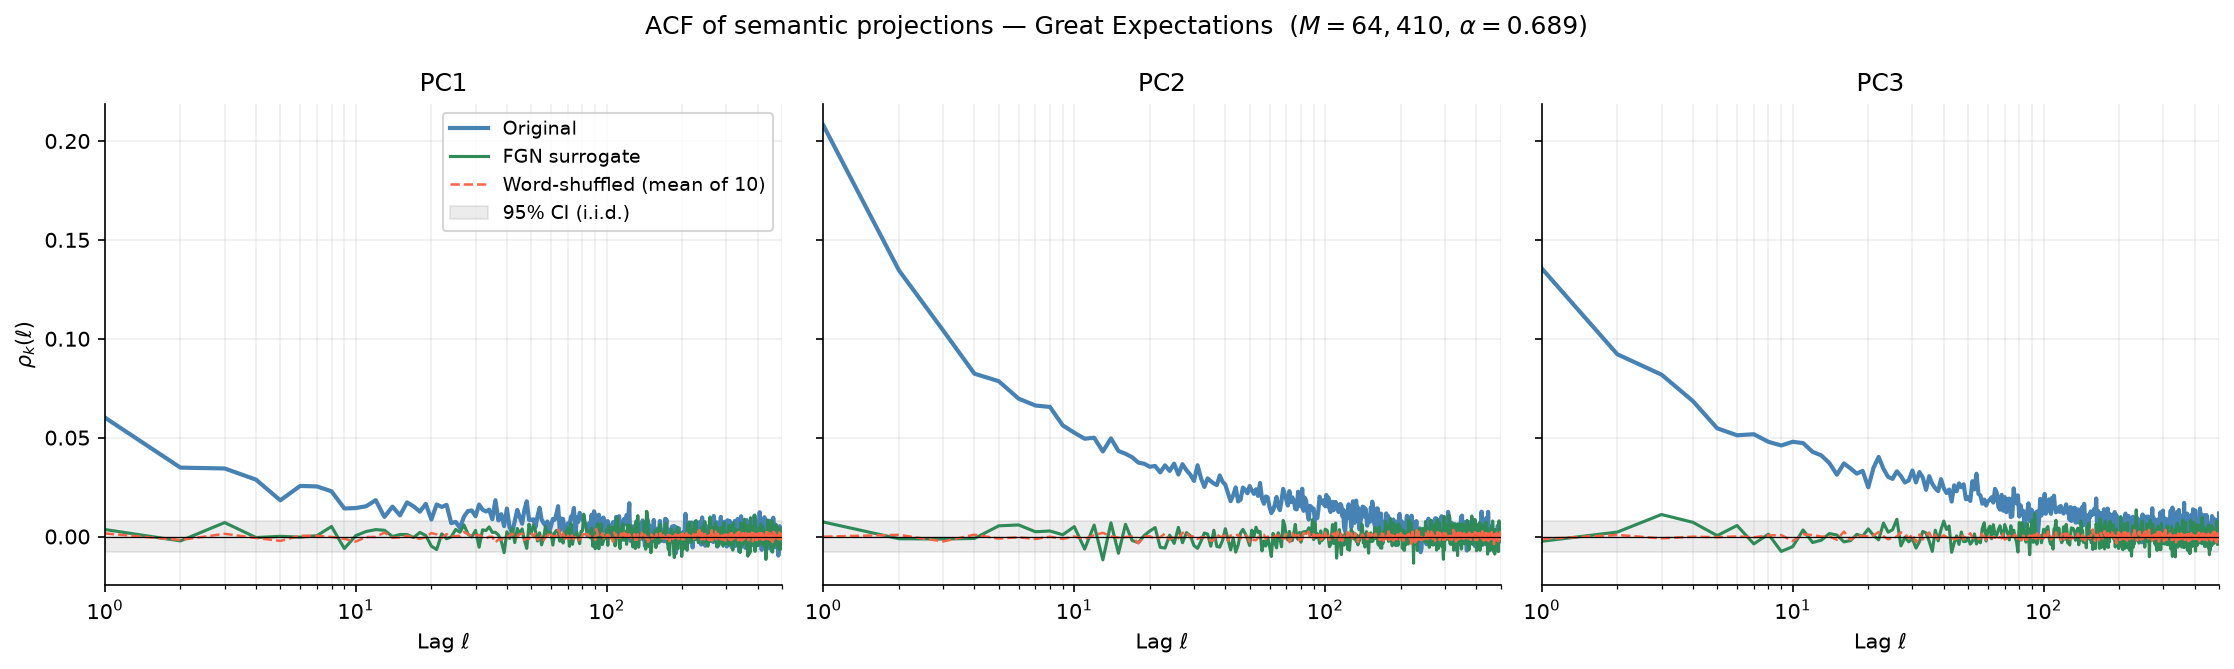
\includegraphics[width=\textwidth]{figures/great_expectations_cut_clean/great_expectations_cut_clean_08_acf_decay_loglag.png}
  \caption{%
    \textbf{Autocorrelation function $\rho_k(\ell)$ of projected
    series, as a function of lag $\ell$ (log scale) ---
    \emph{Great Expectations} (Dickens).}
    Each panel shows one PCA component (PC1, PC2, PC3).
    Blue: original filtered text.
    Green: FGN surrogate.
    Red dashed: word-shuffled null.
    Grey band: $\pm 1.96/\sqrt{M}$ i.i.d.\ reference (95\% CI).
    The original text has substantial positive ACF that decays slowly
    on a log scale, remaining above the i.i.d.\ band up to
    $\ell \sim 100$.
    Both null models collapse immediately into the i.i.d.\ band,
    despite the FGN surrogate having the same DFA exponent
    $\alpha = 0.689$ as the original.
  }
  \label{fig:acf_decay}
\end{figure}

\begin{figure}[htbp]
  \centering
  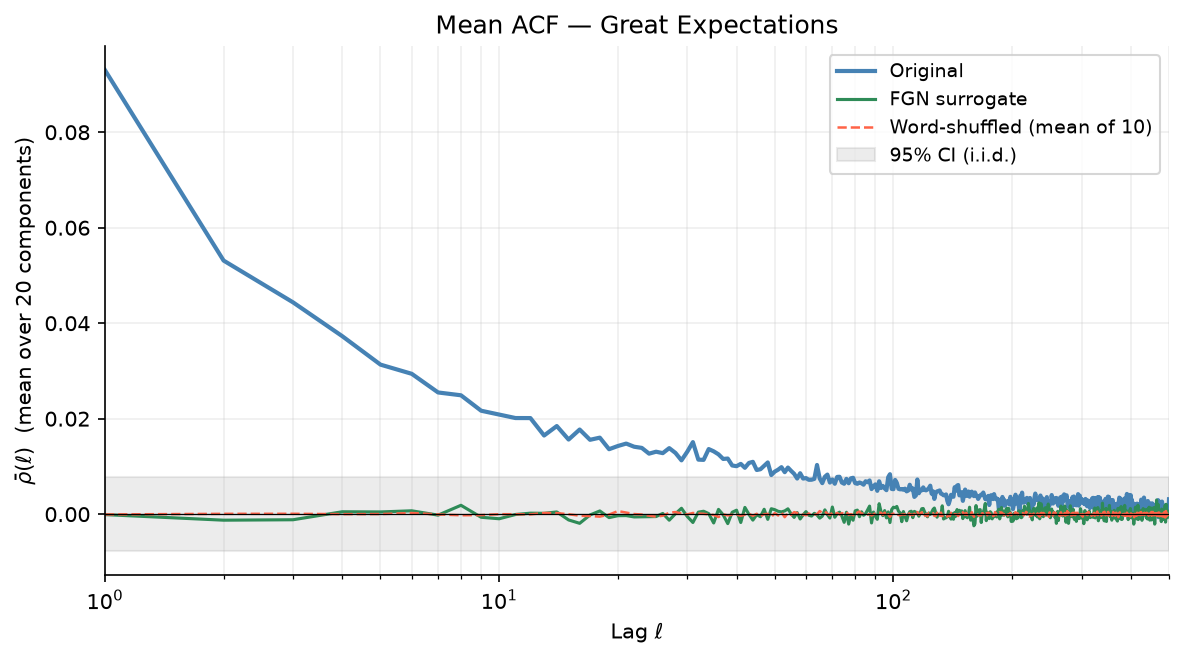
\includegraphics[width=0.72\textwidth]{figures/great_expectations_cut_clean/great_expectations_cut_clean_09_acf_mean_loglag.png}
  \caption{%
    \textbf{Mean ACF $\bar\rho(\ell)$ averaged over all $K=20$ PCA
    components --- \emph{Great Expectations} (Dickens).}
    Same colour conventions as Figure~\ref{fig:acf_decay}.
    The original text maintains positive mean autocorrelation well
    beyond the i.i.d.\ band across the full range of lags shown.
    The FGN surrogate and word-shuffled null are
    indistinguishable from the i.i.d.\ reference at all lags,
    confirming that rank-level long-range memory
    (present in the FGN by construction) does not propagate to the
    semantic projection space.
  }
  \label{fig:acf_mean}
\end{figure}

% ============================================================
%  Subsection: Corpus ACF results
%  Aggiunge a entropy_section_v2.tex dopo sec:acf_results
%  Figures in ./figures/
% ============================================================

\subsection{Corpus-level ACF results}
\label{sec:acf_corpus}

We computed $\rho_k(\ell)$ for all 16 texts and all $K=20$ PCA
components at lags $\ell \in \{1, 2, 5, 10, 20, 50, 100, 200, 300\}$,
yielding $16 \times 20 \times 9 = 2{,}880$ measurements.
The 95\% confidence band for an i.i.d.\ process at sample size $M$
is $\pm 1.96/\sqrt{M}$; since $M$ varies across texts, we use the
text-specific CI for significance tests.

\paragraph{Mean ACF decay.}
Figure~\ref{fig:acf_corpus_decay} shows the mean $\rho(\ell)$ averaged
over all $({\rm text}, k)$ pairs as a function of lag.
The original text maintains positive and significant autocorrelation
across the full range of lags tested, with mean values
\begin{equation}
  \bar\rho^{\rm orig}(1) = 0.100 \pm 0.045,
  \quad
  \bar\rho^{\rm orig}(10) = 0.032 \pm 0.021,
  \quad
  \bar\rho^{\rm orig}(100) = 0.011 \pm 0.011,
  \label{eq:rho_orig_values}
\end{equation}
where $\pm$ denotes one standard deviation over $({\rm text}, k)$
pairs.
The FGN surrogate and the word-shuffled null are indistinguishable
from each other and from zero across all lags:
\begin{equation}
  \bar\rho^{\rm FGN}(1) = 0.002 \pm 0.005,
  \qquad
  \bar\rho^{\rm surr}(1) = 0.000 \pm 0.004.
  \label{eq:rho_null_values}
\end{equation}
The ratio $\bar\rho^{\rm orig}(1) / \bar\rho^{\rm FGN}(1) \approx 50$
quantifies how completely the FGN rank-to-embedding mapping destroys
the frequency-domain long-range correlations in semantic projection
space.

\paragraph{Fraction of significant pairs.}
Figure~\ref{fig:acf_corpus_frac} shows, for each lag, the fraction of
$({\rm text}, k)$ pairs where $|\rho_k(\ell)|$ exceeds the i.i.d.\
band.
At lag $\ell = 1$: $100\%$ of original-text pairs are significant,
$10.9\%$ of FGN pairs, and $4.7\%$ of shuffled pairs.
The FGN figure exceeds the expected false-positive rate
of $5\%$, but the significant cases are concentrated on PC1
(56\% of the PC1 pairs, against 8\% for $k \geq 4$) --- the component
most affected by the geometric artefact of rare transliterated proper
nouns in the GloVe embedding space (Section~\ref{sec:filtering_results}).
From lag $\ell = 2$ onwards the FGN fraction lies between $2.5\%$ and
$7\%$, at the false-positive level. The effect is in any case tiny
relative to the separation of the original projections from both
controls.

The ``original only'' curve (orig significant, FGN not) peaks at
$93\%$ at lag $\ell = 2$ and remains above $50\%$ up to lag
$\ell = 100$, providing a clean corpus-level version of the
single-text result.
The original text maintains detectable semantic autocorrelation
at scales of order $100$ filtered tokens, corresponding to roughly $300$ tokens 
of running text --- a few paragraphs.

\paragraph{Distribution of $\rho_k(1)$.}
Figure~\ref{fig:acf_corpus_rho1} shows the distribution of
$\rho_k(1)$ over all $320$ $({\rm text}, k)$ pairs.
Panel~A shows two completely separated distributions: the original
has $\rho_k(1) \in [0.026, 0.264]$ with mean $0.100$, all
pairs significant; the FGN has $\rho_k(1) \in [-0.014, 0.023]$
with mean $0.002$, the vast majority inside the i.i.d.\ band.

Panel~B zooms on the FGN and shuffled distributions.
Both are centred near zero and overlap substantially.
A one-sample $t$-test of $\bar\rho^{\rm FGN}(1) = 0$ gives
$t = 5.05$, $P < 10^{-6}$: the mean is statistically non-zero but
negligibly small ($0.002$) relative to the orig--null gap ($0.098$).
As with the burstiness differences (Section~\ref{sec:corpus_diffs}),
the statistical significance at this sample size reflects estimator
sensitivity rather than a scientifically meaningful effect.


\begin{remark}
  The residual FGN autocorrelation on PC1 is expected rather than
  anomalous. Rank is an ordering by frequency, so the long-range memory
  imposed on $\mathbf{r}$ is memory along whichever direction of
  embedding space encodes frequency --- and in every text of the corpus
  that direction is PC1, whose poles oppose rare proper nouns and
  transliterations to generic high-frequency vocabulary
  (Section~\ref{sec:semantic_geometry_results}).
  The observation that $56\%$ of PC1 pairs but only $8\%$ of pairs with
  $k \geq 4$ show significant lag-one autocorrelation is therefore the
  signature of rank-level memory reaching the one direction it can
  reach, and failing to reach the thematic ones.
\end{remark}


\begin{figure}[htbp]
  \centering
  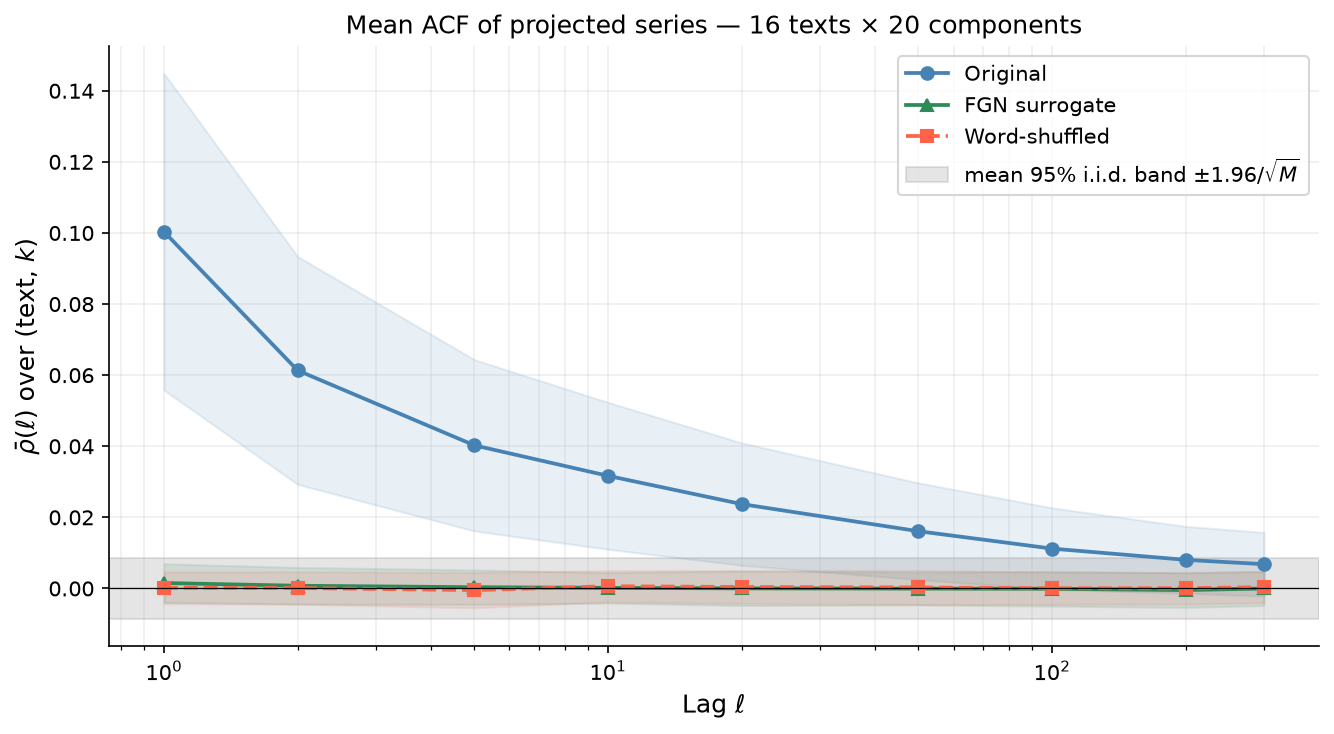
\includegraphics[width=\textwidth]{figures/acf_corpus_mean_decay.png}
  \caption{%
    \textbf{Mean ACF $\bar\rho(\ell)$ of projected series across the
    corpus of 16 texts and $K=20$ components, as a function of lag
    $\ell$ (log scale).}
    Shaded bands: $\pm 1$ standard deviation over
    $({\rm text}, k)$ pairs.
    Grey band: mean 95\% i.i.d.\ confidence band
    $\pm 1.96/\sqrt{M}$.
    Blue circles: original filtered text.
    Green triangles: FGN surrogate.
    Red squares: word-shuffled null.
    The original maintains significant positive ACF across all lags
    tested ($\ell = 1, \ldots, 300$).
    Both null models are indistinguishable from zero at all lags.
  }
  \label{fig:acf_corpus_decay}
\end{figure}

\begin{figure}[htbp]
  \centering
  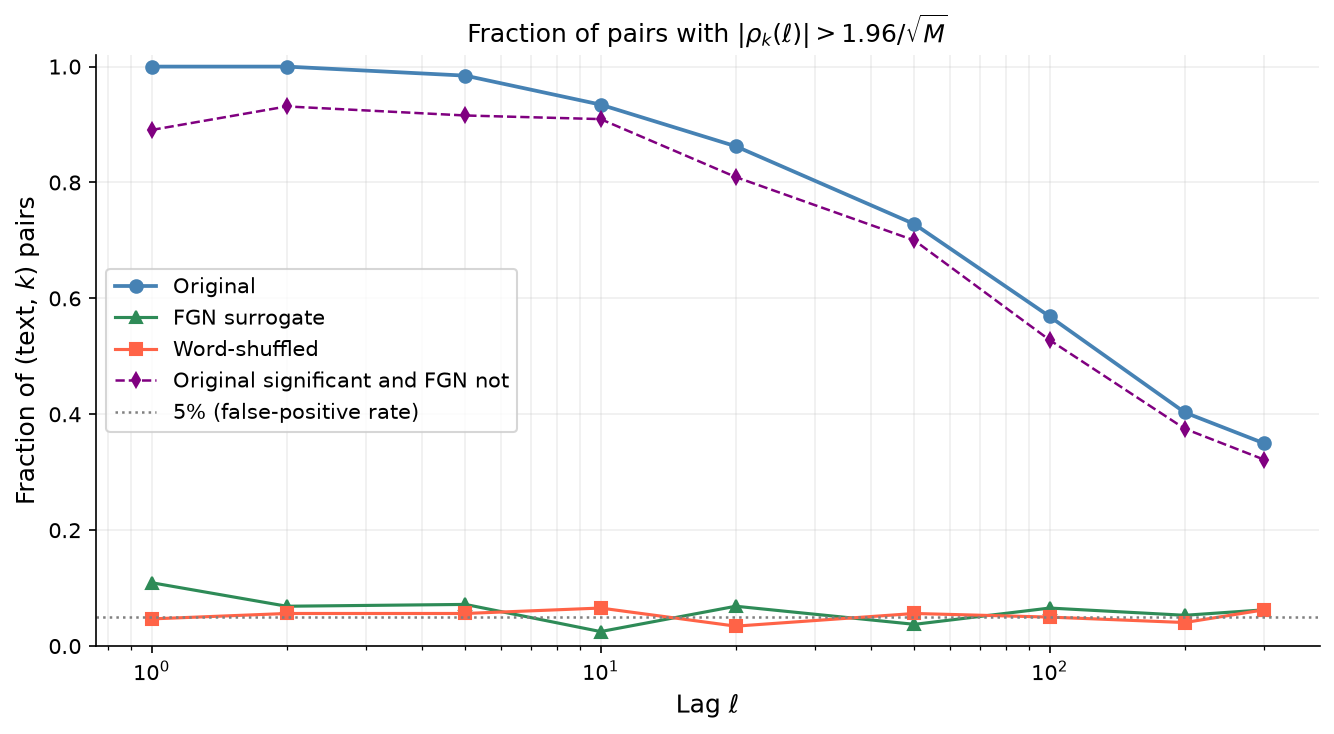
\includegraphics[width=0.72\textwidth]{figures/acf_corpus_frac_significant.png}
  \caption{Fraction of text--component pairs with significant ACF as
  a function of lag $\ell$ (log scale). Blue: original; green: FGN;
  red: word-shuffled; purple dashed: original significant and FGN not.
  The original remains clearly separated from both controls through
  lags of order $10^2$. The short-lag FGN excess is concentrated
  disproportionately in PC1, the component most affected by the
  embedding-geometry artefact discussed in Section~\ref{sec:preprocessing}.}
  \label{fig:acf_corpus_frac}
\end{figure}

\begin{figure}[htbp]
  \centering
  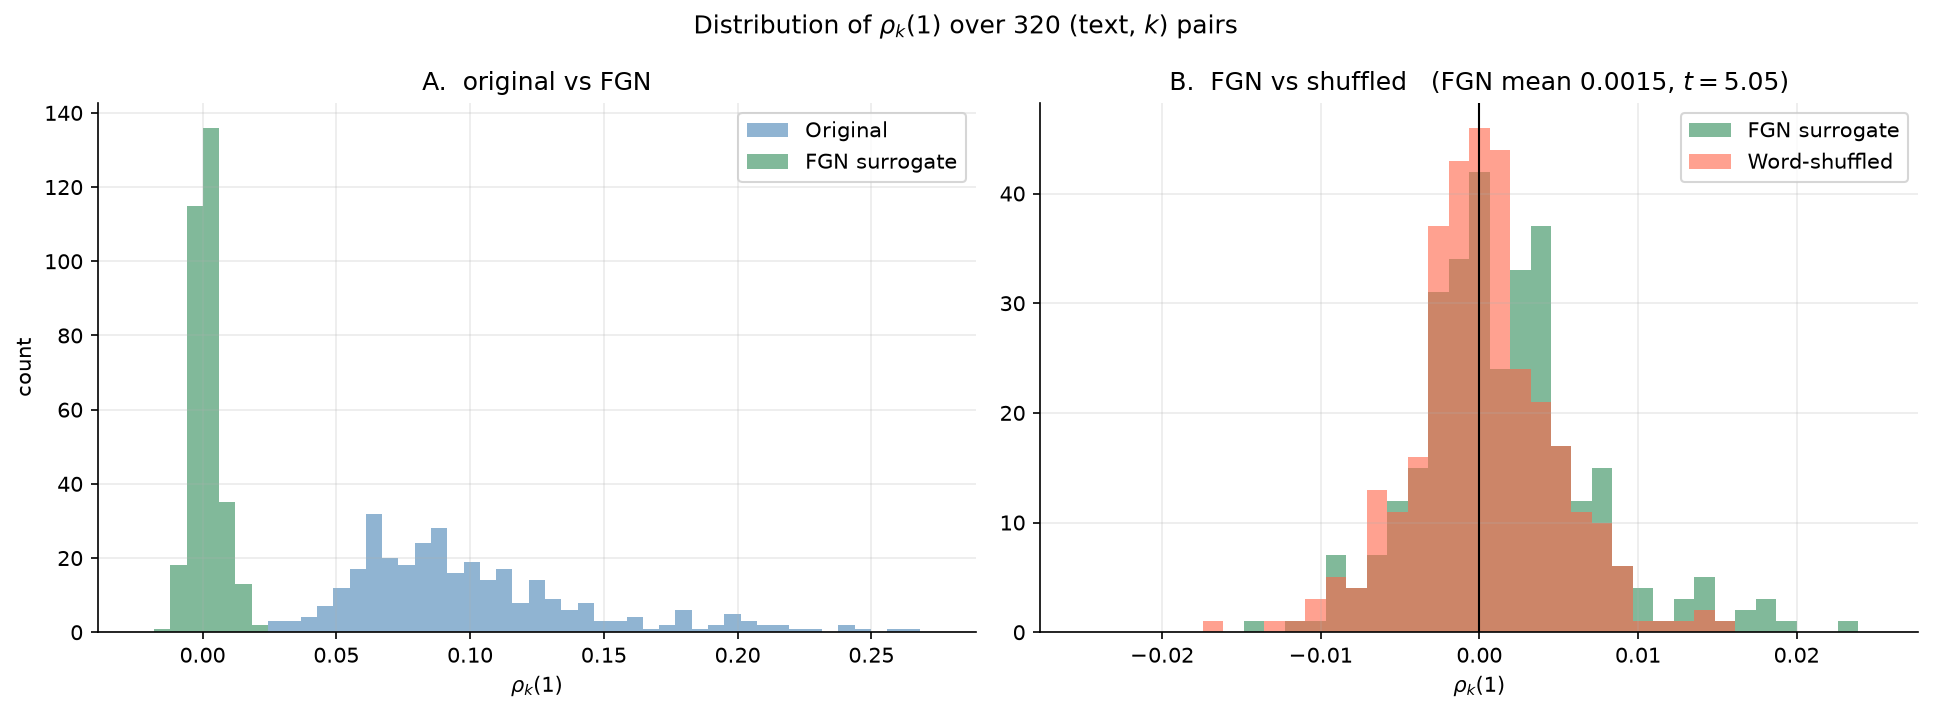
\includegraphics[width=\textwidth]{figures/acf_corpus_rho1_distribution.png}
  \caption{%
    \textbf{Distribution of $\rho_k(1)$ over $320$ (text, $k$) pairs.}
    \textbf{Panel A}: original (blue) and FGN (green).
    The two distributions are completely separated: every original pair
    exceeds its own text-specific i.i.d.\ band (which ranges from
    $0.004$ to $0.015$ across the corpus), while nearly all FGN pairs
    fall inside it.
    \textbf{Panel B}: FGN (green) and word-shuffled (red) on an
    expanded scale.
    Both are centred near zero; a $t$-test gives $t = 5.05$
    for $\bar\rho^{\rm FGN}(1) = 0$ but the effect size is
    negligible ($0.002$) relative to the orig--null gap ($0.098$).
  }
  \label{fig:acf_corpus_rho1}
\end{figure}

% ============================================================
%  Subsection: DFA of projected series
%  Si aggiunge a entropy_section_v2.tex dopo sec:acf_corpus
%  Figures in ./figures/
% ============================================================

\subsection{DFA of projected series}
\label{sec:dfa_projections}

The ACF results of Sections~\ref{sec:acf_results}
and~\ref{sec:acf_corpus} confirm the predicted ordering
$\rho_k^{\rm orig}(\ell) \gg \rho_k^{\rm FGN}(\ell) \approx
\rho_k^{\rm surr}(\ell) \approx 0$.
We now complement the ACF analysis by computing the DFA scaling
exponent of the projected series $x_t^{(k)}$ directly, providing the
semantic-level analogue of the
symbolic-level DFA result that motivates the paper.

For each PCA component $k$ and each of the three series
(original, FGN, word-shuffled), we apply DFA to the scalar
time series $x_t^{(k)}$ and estimate the scaling exponent
$\alpha_k$ from $F(s) \sim s^{\alpha_k}$, where $F(s)$ is the
detrended fluctuation function at box size $s$.
Box sizes range from $s_{\min} = 10$ to $s_{\max} = M/4$
on a logarithmic grid.

\paragraph{Results on Great Expectations.}
Table~\ref{tab:dfa_proj} and Figure~\ref{fig:dfa_spectrum}
report $\alpha_k$ for all $K = 20$ components of
\emph{Great Expectations} by Dickens ($\alpha = 0.689$).
The results confirm the prediction precisely:

\begin{itemize}
  \item \textbf{Original}: $\alpha_k^{\rm orig} > 0.5$ in all
        $20/20$ components, with mean
        $\bar\alpha^{\rm orig} = 0.623 \pm 0.034$.
        All values exceed the shuffled reference by more than
        $2\sigma$, confirming long-range correlations in every
        semantic projection.

  \item \textbf{FGN surrogate}: $|\alpha_k^{\rm FGN} - 0.5| < 0.05$
        in all $20/20$ components, with mean
        $\bar\alpha^{\rm FGN} = 0.499 \pm 0.014$.
        Despite having a matched DFA exponent ($\alpha=0.689$,
        generator exponent $\alpha_0=0.74$) in the rank sequence
        by construction, the FGN projects
        onto every semantic direction as an uncorrelated process.

  \item \textbf{Word-shuffled}: $\bar\alpha^{\rm surr} =
        0.499 \pm 0.004$, consistent with $\alpha = 0.5$
        (white noise) as expected for an i.i.d.\ sequence.
\end{itemize}

\begin{table}[htbp]
\centering
\caption{DFA scaling exponents $\alpha_k$ of projected series
$x_t^{(k)}$ for \emph{Great Expectations} (Dickens, $\alpha=0.689$).
Every original value exceeds the shuffled reference by more than
$2\sigma$ (the spread over the ten shuffled realisations is
$\sigma\simeq0.004$), and every FGN value lies within $0.05$ of $0.5$.}
\label{tab:dfa_proj}
\scriptsize
\setlength{\tabcolsep}{4pt}
\begin{tabular}{r ccc r ccc}
\toprule
$k$ & $\alpha^{\rm orig}$ & $\alpha^{\rm FGN}$ &
    $\alpha^{\rm surr}$ &
$k$ & $\alpha^{\rm orig}$ & $\alpha^{\rm FGN}$ &
    $\alpha^{\rm surr}$ \\
\midrule
 1 & 0.605 & 0.511$\sim$ & 0.501 &
11 & 0.57 & 0.506$\sim$ & 0.500 \\
 2 & 0.681 & 0.500$\sim$ & 0.491 &
12 & 0.642 & 0.493$\sim$ & 0.502 \\
 3 & 0.693 & 0.518$\sim$ & 0.495 &
13 & 0.564 & 0.512$\sim$ & 0.500 \\
 4 & 0.634 & 0.514$\sim$ & 0.499 &
14 & 0.595 & 0.484$\sim$ & 0.497 \\
 5 & 0.64 & 0.486$\sim$ & 0.496 &
15 & 0.645 & 0.486$\sim$ & 0.497 \\
 6 & 0.633 & 0.515$\sim$ & 0.501 &
16 & 0.579 & 0.505$\sim$ & 0.494 \\
 7 & 0.647 & 0.504$\sim$ & 0.498 &
17 & 0.586 & 0.511$\sim$ & 0.493 \\
 8 & 0.633 & 0.469$\sim$ & 0.497 &
18 & 0.617 & 0.515$\sim$ & 0.507 \\
 9 & 0.643 & 0.482$\sim$ & 0.494 &
19 & 0.595 & 0.489$\sim$ & 0.505 \\
10 & 0.630 & 0.482$\sim$ & 0.503 &
20 & 0.622 & 0.495$\sim$ & 0.502 \\
\midrule
\multicolumn{4}{l}{\textbf{Mean}} &
\multicolumn{4}{l}{$\bar\alpha^{\rm orig}=0.623\pm0.034$ \quad
                   $\bar\alpha^{\rm FGN}=0.499\pm0.014$ \quad
                   $\bar\alpha^{\rm surr}=0.499\pm0.004$}\\
\bottomrule
\end{tabular}
\end{table}

Figure~\ref{fig:dfa_loglog} shows the log-log fluctuation
function $F(s)$ for PC1, PC2, and PC3.
The original text shows a clear power-law scaling with
slope $\alpha_k \approx 0.60$--$0.69$, visibly steeper than
the reference slope $0.5$.
The FGN and shuffled curves are parallel to the reference slope,
confirming $\alpha_k \approx 0.5$ for both null models.

\begin{remark}
  The exponents $\alpha_k^{\rm orig} \in [0.564, 0.693]$ do not
  decrease monotonically with $k$: PC12 ($\alpha=0.642$) and PC15
  ($\alpha=0.645$) exceed PC1 ($\alpha=0.605$), even though they carry
  an order of magnitude less variance.
  This partial decorrelation between PCA rank (ordered by variance) and
  DFA exponent mirrors the decorrelation between the eigenvalue
  spectrum $\{\lambda_k\}$ and the burstiness spectrum $\{B_k\}$
  reported in Section~\ref{sec:oliver}: semantic variance and semantic
  temporal structure are distinct properties of narrative
  organisation.
\end{remark}

\paragraph{Consistent temporal signatures.}
The DFA, ACF, and burstiness analyses provide mutually consistent but
non-equivalent summaries of temporal organisation. For the original
projections, $\alpha_k>0.5$, the ACF remains positive over extended
lags, and $B_k$ exceeds the geometric reference. For both controls,
$\alpha_k\simeq0.5$, the ACF is close to zero, and
$B_k\simeq\CV_{\rm geom}$. These observations can be summarised as
\begin{equation}
  \alpha_k^{\rm orig}>0.5,
  \qquad \rho_k^{\rm orig}(\ell)>0\ \text{over extended lags},
  \qquad B_k^{\rm orig}>\CV_{\rm geom},
  \label{eq:chain_numbers}
\end{equation}
whereas the FGN and shuffled projections remain close to their
uncorrelated references in all three measures.

The FGN surrogate is especially informative because its rank sequence
has the prescribed long-range DFA exponent, while every analysed
semantic projection has $\alpha_k^{\rm FGN}\simeq0.5$. Rank-level
persistence therefore does not propagate automatically into semantic
projection space.

\begin{figure}[htbp]
  \centering
  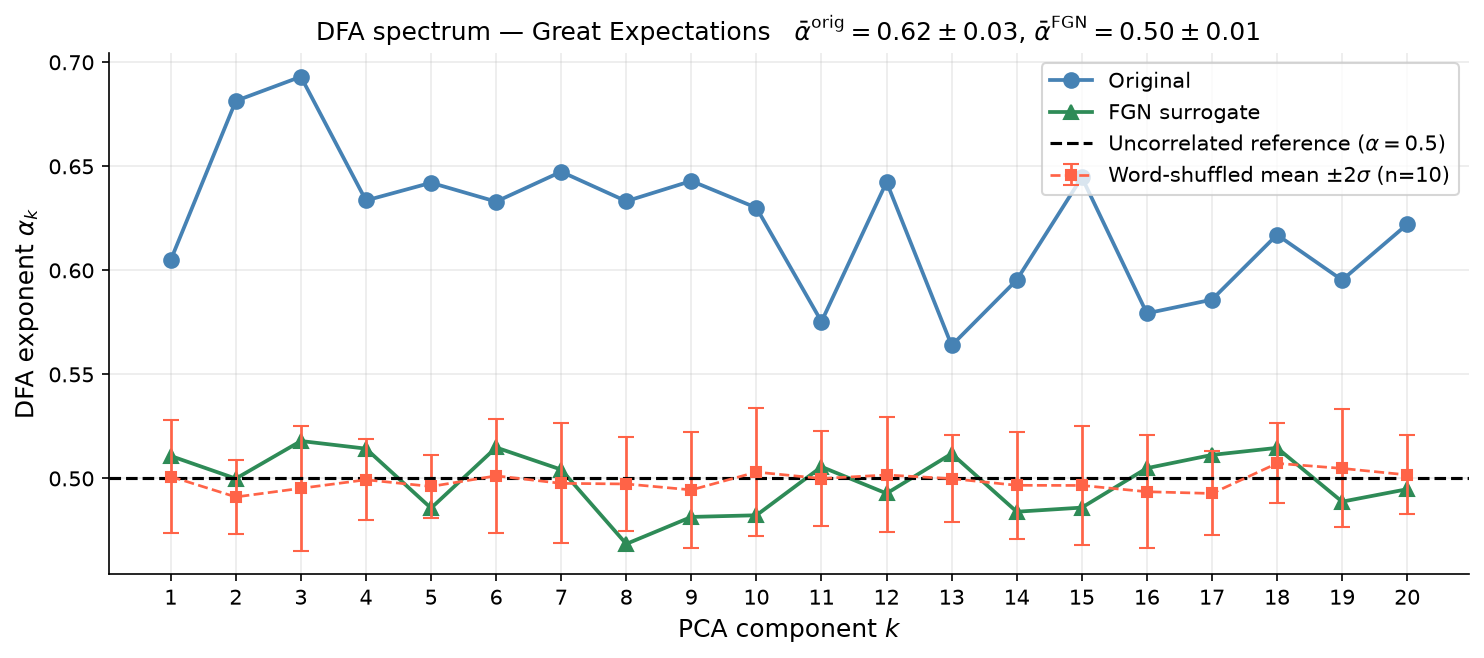
\includegraphics[width=\textwidth]{figures/great_expectations_cut_clean/great_expectations_cut_clean_10_dfa_projections_spectrum.png}
  \caption{%
    \textbf{DFA scaling exponent $\alpha_k$ of projected series
    $x_t^{(k)}$ as a function of PCA component $k$ ---
    \emph{Great Expectations} (Dickens).}
    Blue circles: original filtered text.
    Green triangles: FGN surrogate.
    Red squares: word-shuffled null (mean $\pm 2\sigma$
    over 10 realisations).
    Dashed line: uncorrelated reference $\alpha = 0.5$.
    The original text has $\alpha_k > 0.5$ for all 20 components;
    the FGN and shuffled are indistinguishable from $\alpha = 0.5$.
  }
  \label{fig:dfa_spectrum}
\end{figure}

\begin{figure}[htbp]
  \centering
  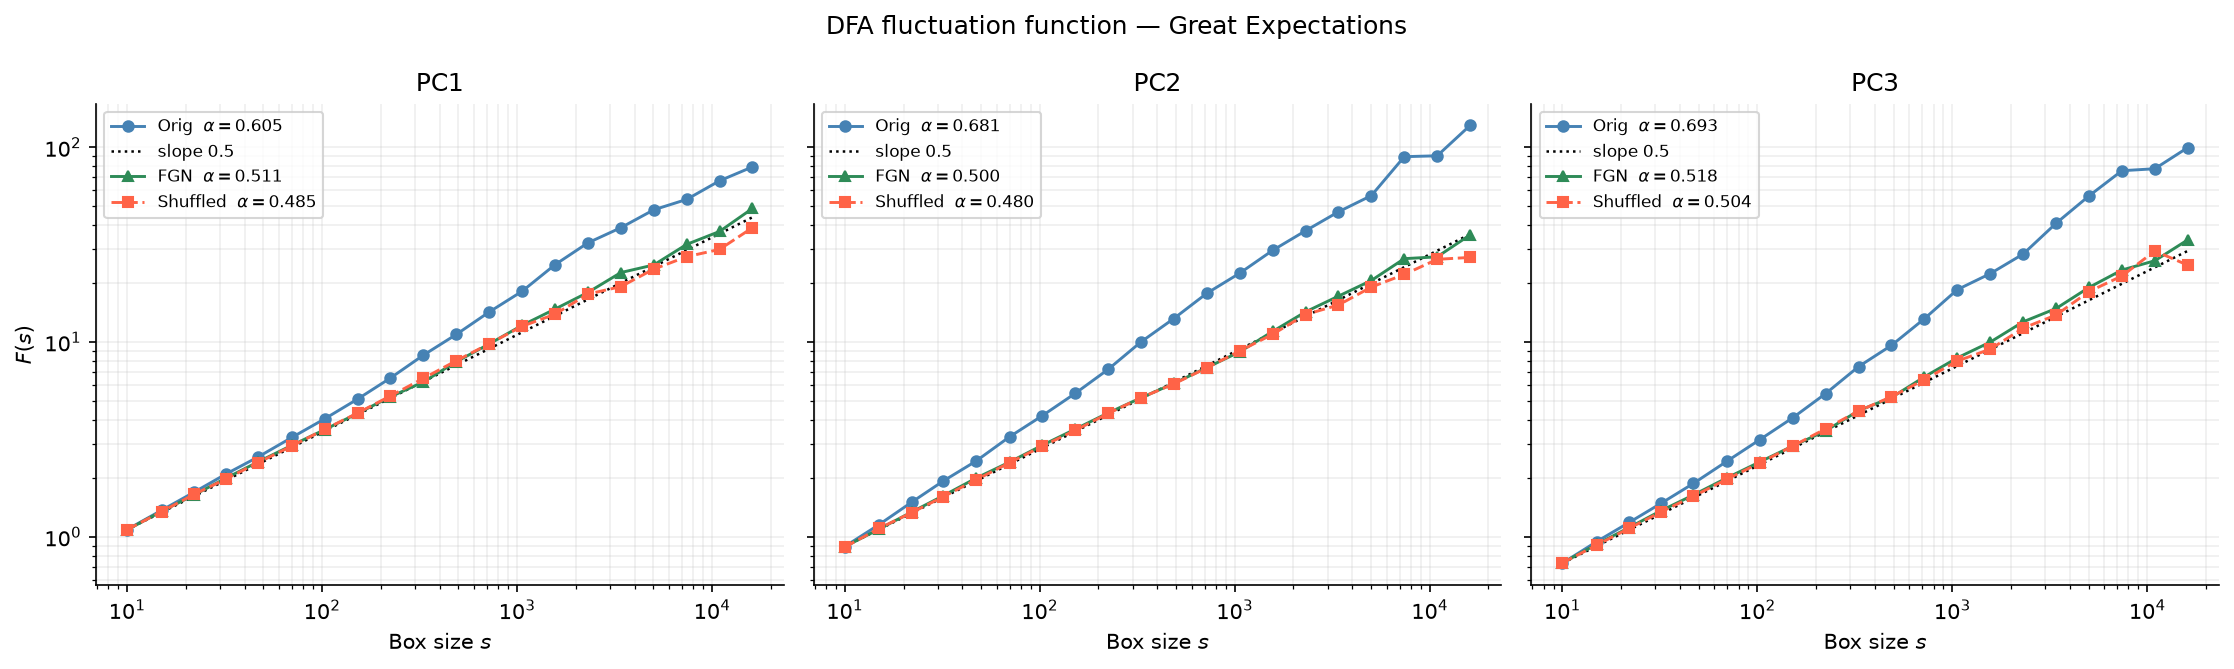
\includegraphics[width=\textwidth]{figures/great_expectations_cut_clean/great_expectations_cut_clean_11_dfa_projections_loglog.png}
  \caption{%
    \textbf{Log-log DFA fluctuation function $F(s)$ for PC1, PC2,
    and PC3 --- \emph{Great Expectations} (Dickens).}
    Each panel shows one component; the estimated exponent
    $\alpha_k$ is given in the legend.
    Dotted line: reference slope $0.5$.
    The original text (blue) has a consistently steeper slope
    than both null models, which are parallel to the $\alpha=0.5$
    reference across all box sizes $s$.
  }
  \label{fig:dfa_loglog}
\end{figure}
\subsection{Connection between ACF and burstiness}
\label{sec:acf_burstiness_connection}

The ACF and the burstiness parameter probe different aspects of the
same projected series. By the Wiener--Khintchine theorem, slow ACF
decay is associated with excess low-frequency power in the spectral
density
\begin{equation}
  S_k(\omega)=\sum_{\ell=-\infty}^{\infty}
  \rho_k(\ell)e^{-i\omega\ell}.
  \label{eq:projection_spectrum}
\end{equation}
Such low-frequency variation is consistent with extended semantic
episodes and clustered threshold exceedances, and therefore with broad
IET distributions; in the long-range correlated case the sum
in~\eqref{eq:projection_spectrum} diverges as $\omega\to0$, which is
the spectral expression of that persistence.The connection is not one-to-one, however:
thresholding is non-linear, and $B_k$ depends on temporal structure
beyond the second-order information contained in the ACF.



The empirical conclusion is consequently based on the agreement of
three complementary observations rather than on a deterministic causal
identity. Original texts show elevated $B_k$, positive projection ACFs,
and projection DFA exponents above $0.5$. The FGN and word-shuffled controls remain 
close to the geometric
baseline in burstiness, to zero in autocorrelation, and to white noise
in DFA. This convergence of measures supports the
interpretation that ordered topical organisation, rather than global
rank-level scaling alone, produces persistence in semantic projection
space.

\FloatBarrier
% ------------------------------------------------------------
\section{Discussion and Conclusions}
\label{sec:discussion}

%\TODO{Write discussion. Results from all sections are now available.
%  Key points:
%  - Extension of Altmann 2012: from word-level to topic-level burstiness
%    via PCA of embedding trajectories
%  - Two routes to the same DFA exponent: non-stationary burstiness
%    (real texts) vs stationary FGN. Distinction is now fully documented
%    at three levels: $B_k, rho_k(ell), alpha_k$ of projections
%  - The taxonomy table (Sec.~2.7) as organising principle
%  - PC1 artefact: to be resolved with higher MAX\_FREQ\_RANK
%  - Limitations: static embeddings, English-only corpus,
%    single FGN realisation per text
%  - Future: contextual embeddings, multilingual corpus,
%    block entropy estimation, DFA of projections for full corpus
%}
%
%\section{Sensitivity Analysis}
%\label{sec:sensitivity}
%
%\NOTE{Results already available in \texttt{corpus\_burstiness.csv}
%(6 values of $q$ from 0.60 to 0.99).
%The full-ordering fraction is $\geq 99.4\%$ for $q \in [0.60, 0.95]$
%and $98.4\%$ at $q = 0.99$ (see Section~\ref{sec:corpus_robustness}
%and Figure~\ref{fig:corpus_robustness}).
%\TODO{Add per-k heatmap figure from quantile sweep notebook cell.}}


\section*{CRediT authorship contribution statement}
\textbf{Mirko Degli Esposti:} Conceptualization, Methodology, Software,
Formal analysis, Writing -- original draft, Writing -- review \& editing.
\textbf{Marcelo A.\ Montemurro:} Conceptualization, Methodology,
Formal analysis, Writing -- review \& editing.
% Adjust to the actual division of work before submission.
 
\section*{Declaration of competing interest}
The authors declare that they have no known competing financial
interests or personal relationships that could have appeared to
influence the work reported in this paper.
 
\section*{Declaration of generative AI in the writing process}
% Required by Elsevier when applicable; delete if not applicable.
During the preparation of this work the authors used a large language
model to assist with code refactoring and manuscript editing. The
authors reviewed and edited the content as needed and take full
responsibility for the content of the published article.
 
\section*{Data availability}
All texts are public-domain works from Project Gutenberg. The corpus,
the analysis code, the result tables and the scripts that regenerate
every figure in this paper are available at
\url{https://github.com/mirko-degli-esposti/semantic-burstiness-texts}.
Pre-trained GloVe vectors are distributed by Stanford NLP
\citep{Pennington2014}.


\section*{Acknowledgements}
% funding, colleagues, computing resources
\appendix

\section{Geometric distribution as IET null: derivation}
\label{app:geometric}

Consider a binary sequence $b_1, b_2, \ldots, b_M$ where each $b_t$
is independently Bernoulli$(p)$.
An \emph{event} occurs at position $t$ when $b_t = 1$.
The inter-event time $\tau$ between two successive events is the number
of positions (including the terminal event) from one event to the next.
The probability of $\tau = k$ requires $b_{t+1} = \cdots = b_{t+k-1}
= 0$ and $b_{t+k} = 1$:
\begin{equation}
  \Pr(\tau = k) = (1-p)^{k-1}\,p, \qquad k = 1, 2, 3, \ldots
\end{equation}
which is the geometric distribution with parameter $p$.
Its mean, variance, and coefficient of variation are
\begin{equation}
  \meantau = \frac{1}{p},
  \qquad
  \mathrm{Var}(\tau) = \frac{1-p}{p^2},
  \qquad
  \CV_{\rm geom}(p) = \sqrt{1-p}.
\end{equation}
The exponential distribution $p(\tau) \propto e^{-\lambda\tau}$ arises
in the limit $p \to 0$ with $\lambda = -\log(1-p) \approx p$, and has
$\CV = 1$ (Poisson process).
For $p = 0.05$, $\CV_{\rm geom} = 0.975 \approx 1$, so the Poisson
approximation is adequate.
For $p = 0.5$, $\CV_{\rm geom} = 0.707$, and the Poisson
approximation fails badly.

\section{Additional per-text figures}
\label{app:pertext}

Eigenvalue spectra and inter-event-time distributions for the three
representative texts other than \emph{War and Peace}, whose
corresponding figures appear in the main text
(Figures~\ref{fig:wrnpc_spectra} and~\ref{fig:wrnpc_iet}).
Equivalent figures for every text of the corpus, at any threshold
quantile, can be regenerated with \texttt{scripts/run\_text.py} in the
code repository.

\begin{figure}[htbp]
  \centering
  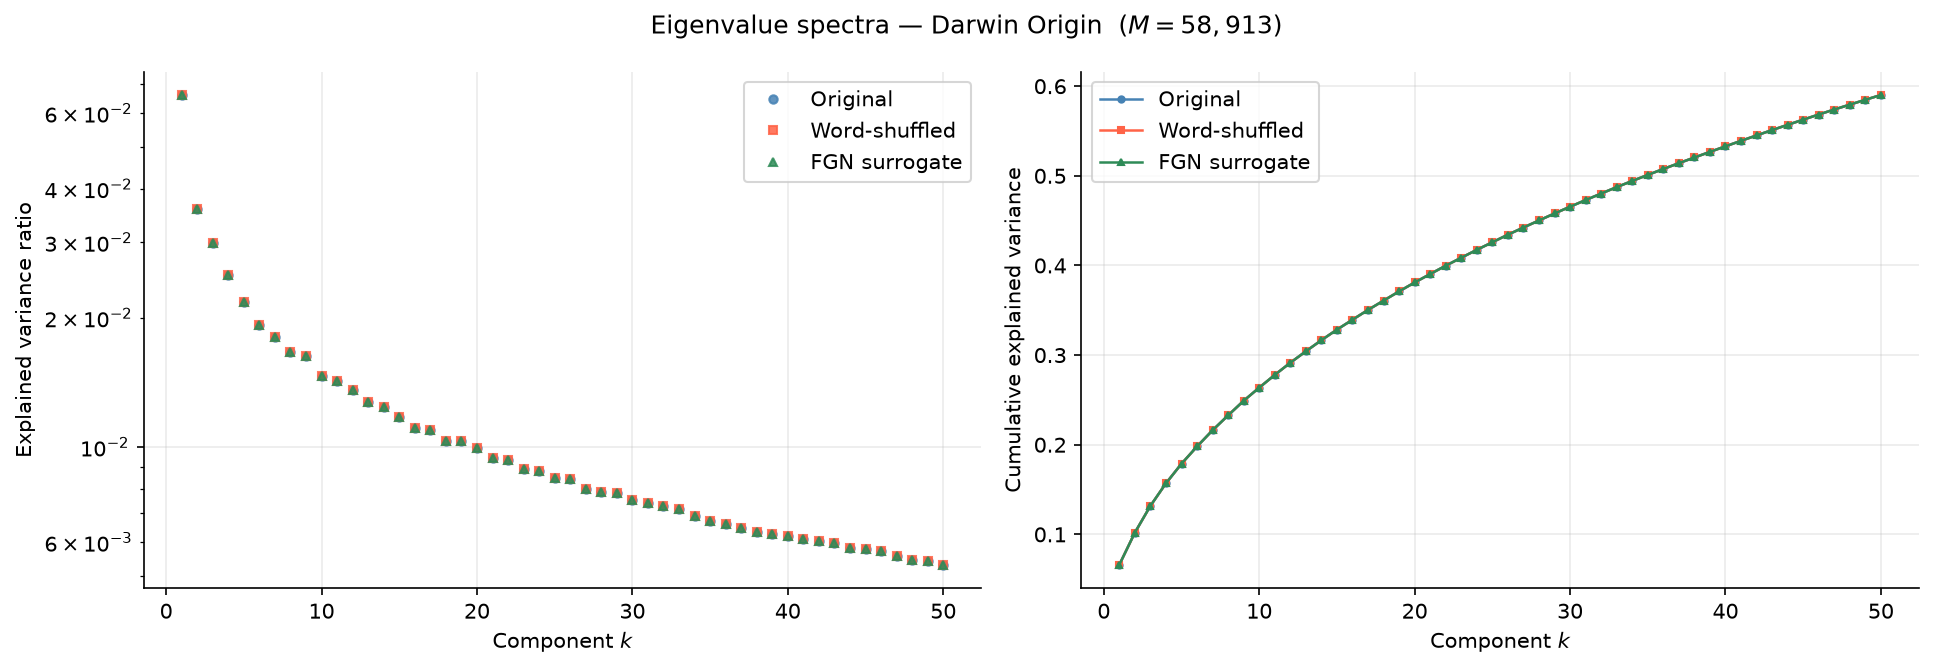
\includegraphics[width=\textwidth]{figures/darwin_origin/darwin_origin_02_spectra_comparison.png}
  \caption{Eigenvalue spectra and cumulative explained variance
  for \emph{On the Origin of Species}.
  Same conventions as Figure~\ref{fig:wrnpc_spectra}.}
  \label{fig:darwin_spectra}
\end{figure}

\begin{figure}[htbp]
  \centering
  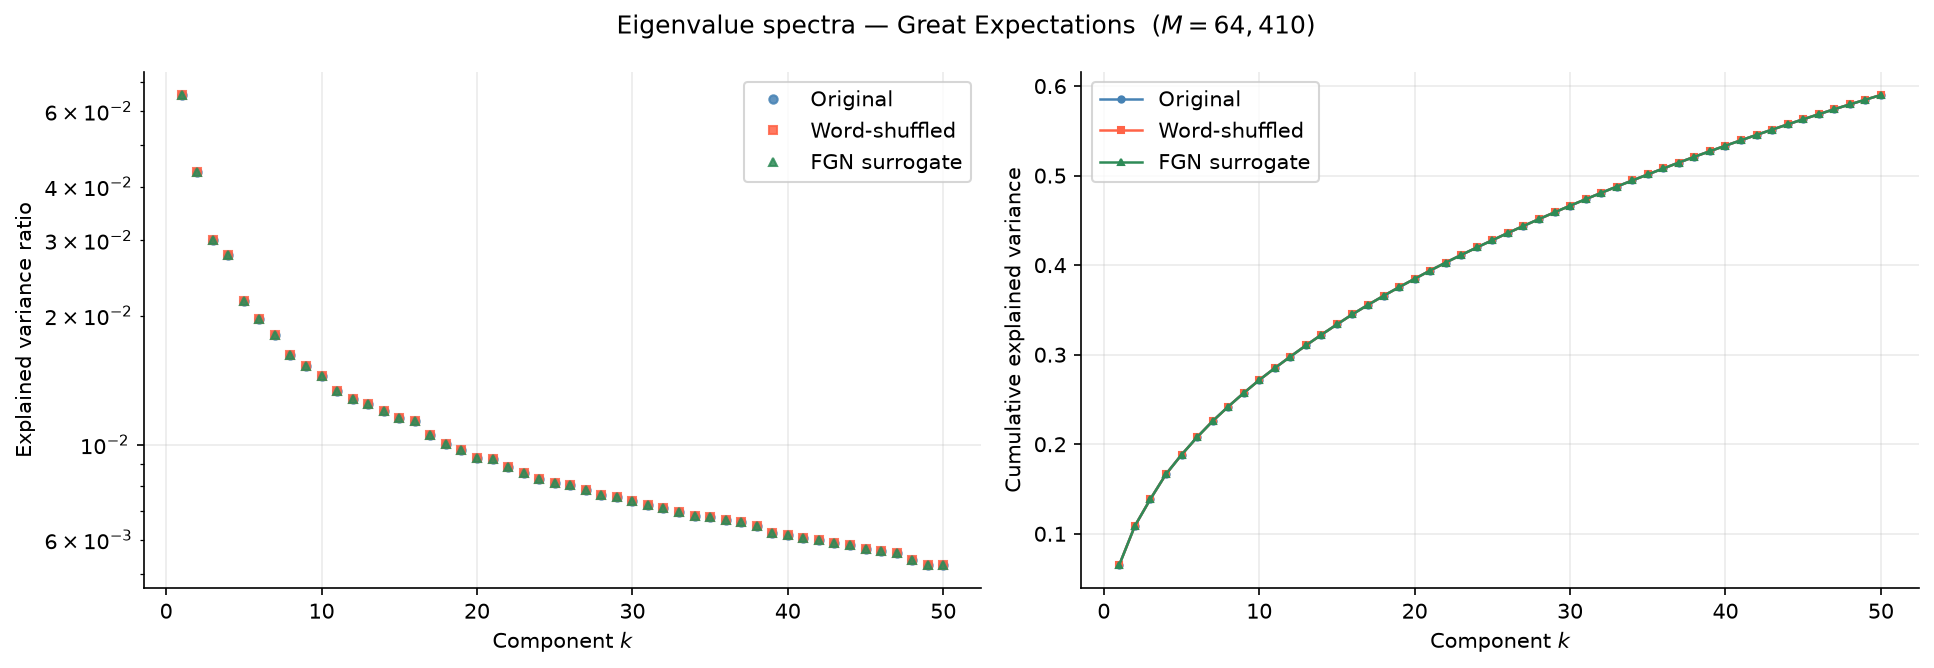
\includegraphics[width=\textwidth]{figures/great_expectations_cut_clean/great_expectations_cut_clean_02_spectra_comparison.png}
  \caption{Eigenvalue spectra and cumulative explained variance
  for \emph{Great Expectations}.
  Same conventions as Figure~\ref{fig:wrnpc_spectra}.}
  \label{fig:greatexp_spectra}
\end{figure}

\begin{figure}[htbp]
  \centering
  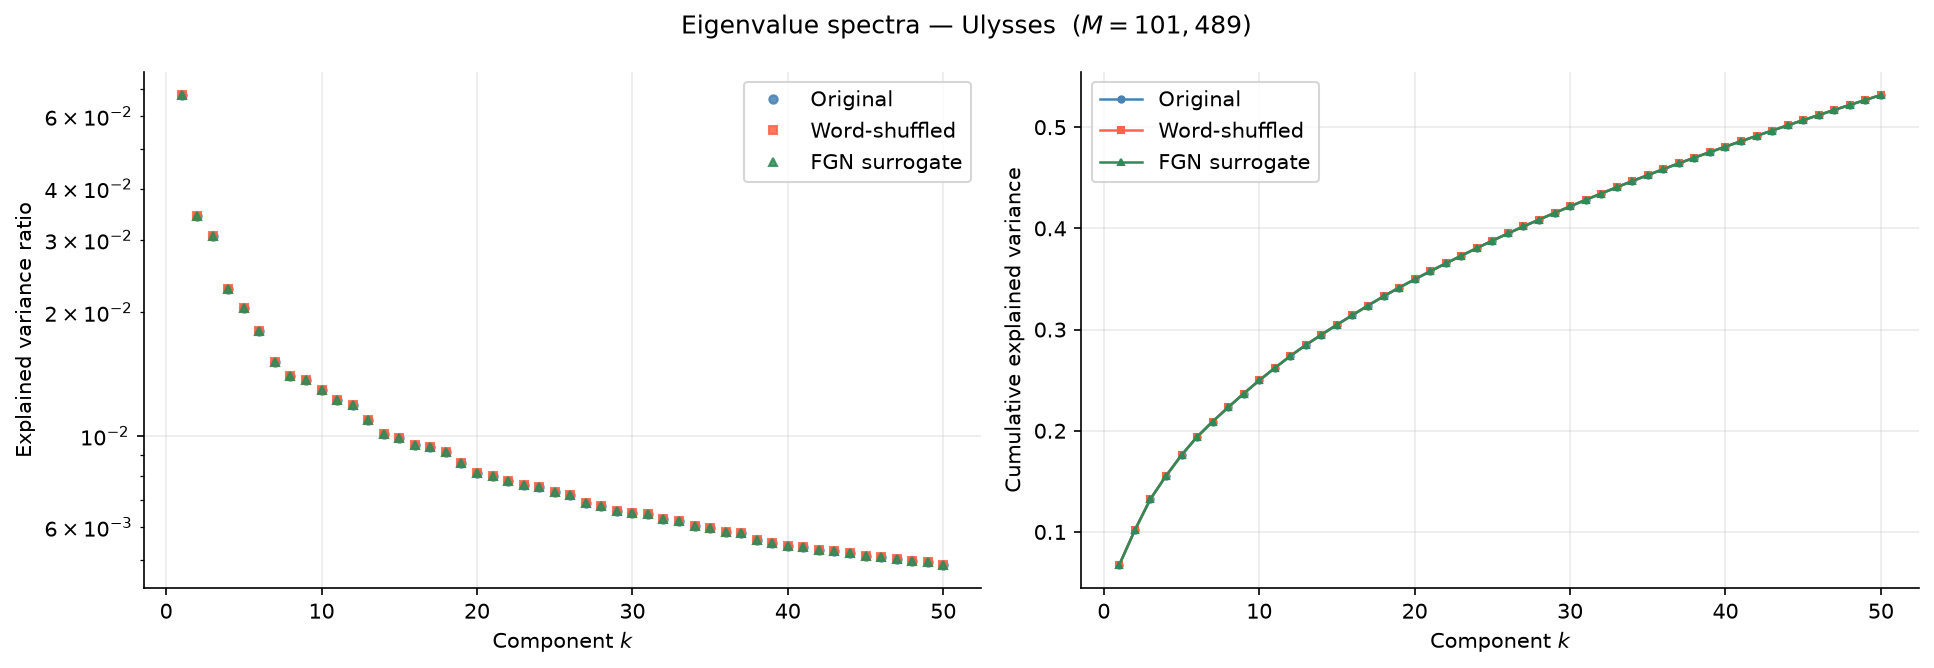
\includegraphics[width=\textwidth]{figures/eng_ulysses/eng_ulysses_02_spectra_comparison.png}
  \caption{Eigenvalue spectra and cumulative explained variance
  for \emph{Ulysses}.
  The more gradual eigenvalue decay reflects the greater stylistic
  diversity of the 18 episodes compared to the other texts.}
  \label{fig:ulysses_spectra}
\end{figure}

\begin{figure}[htbp]
  \centering
  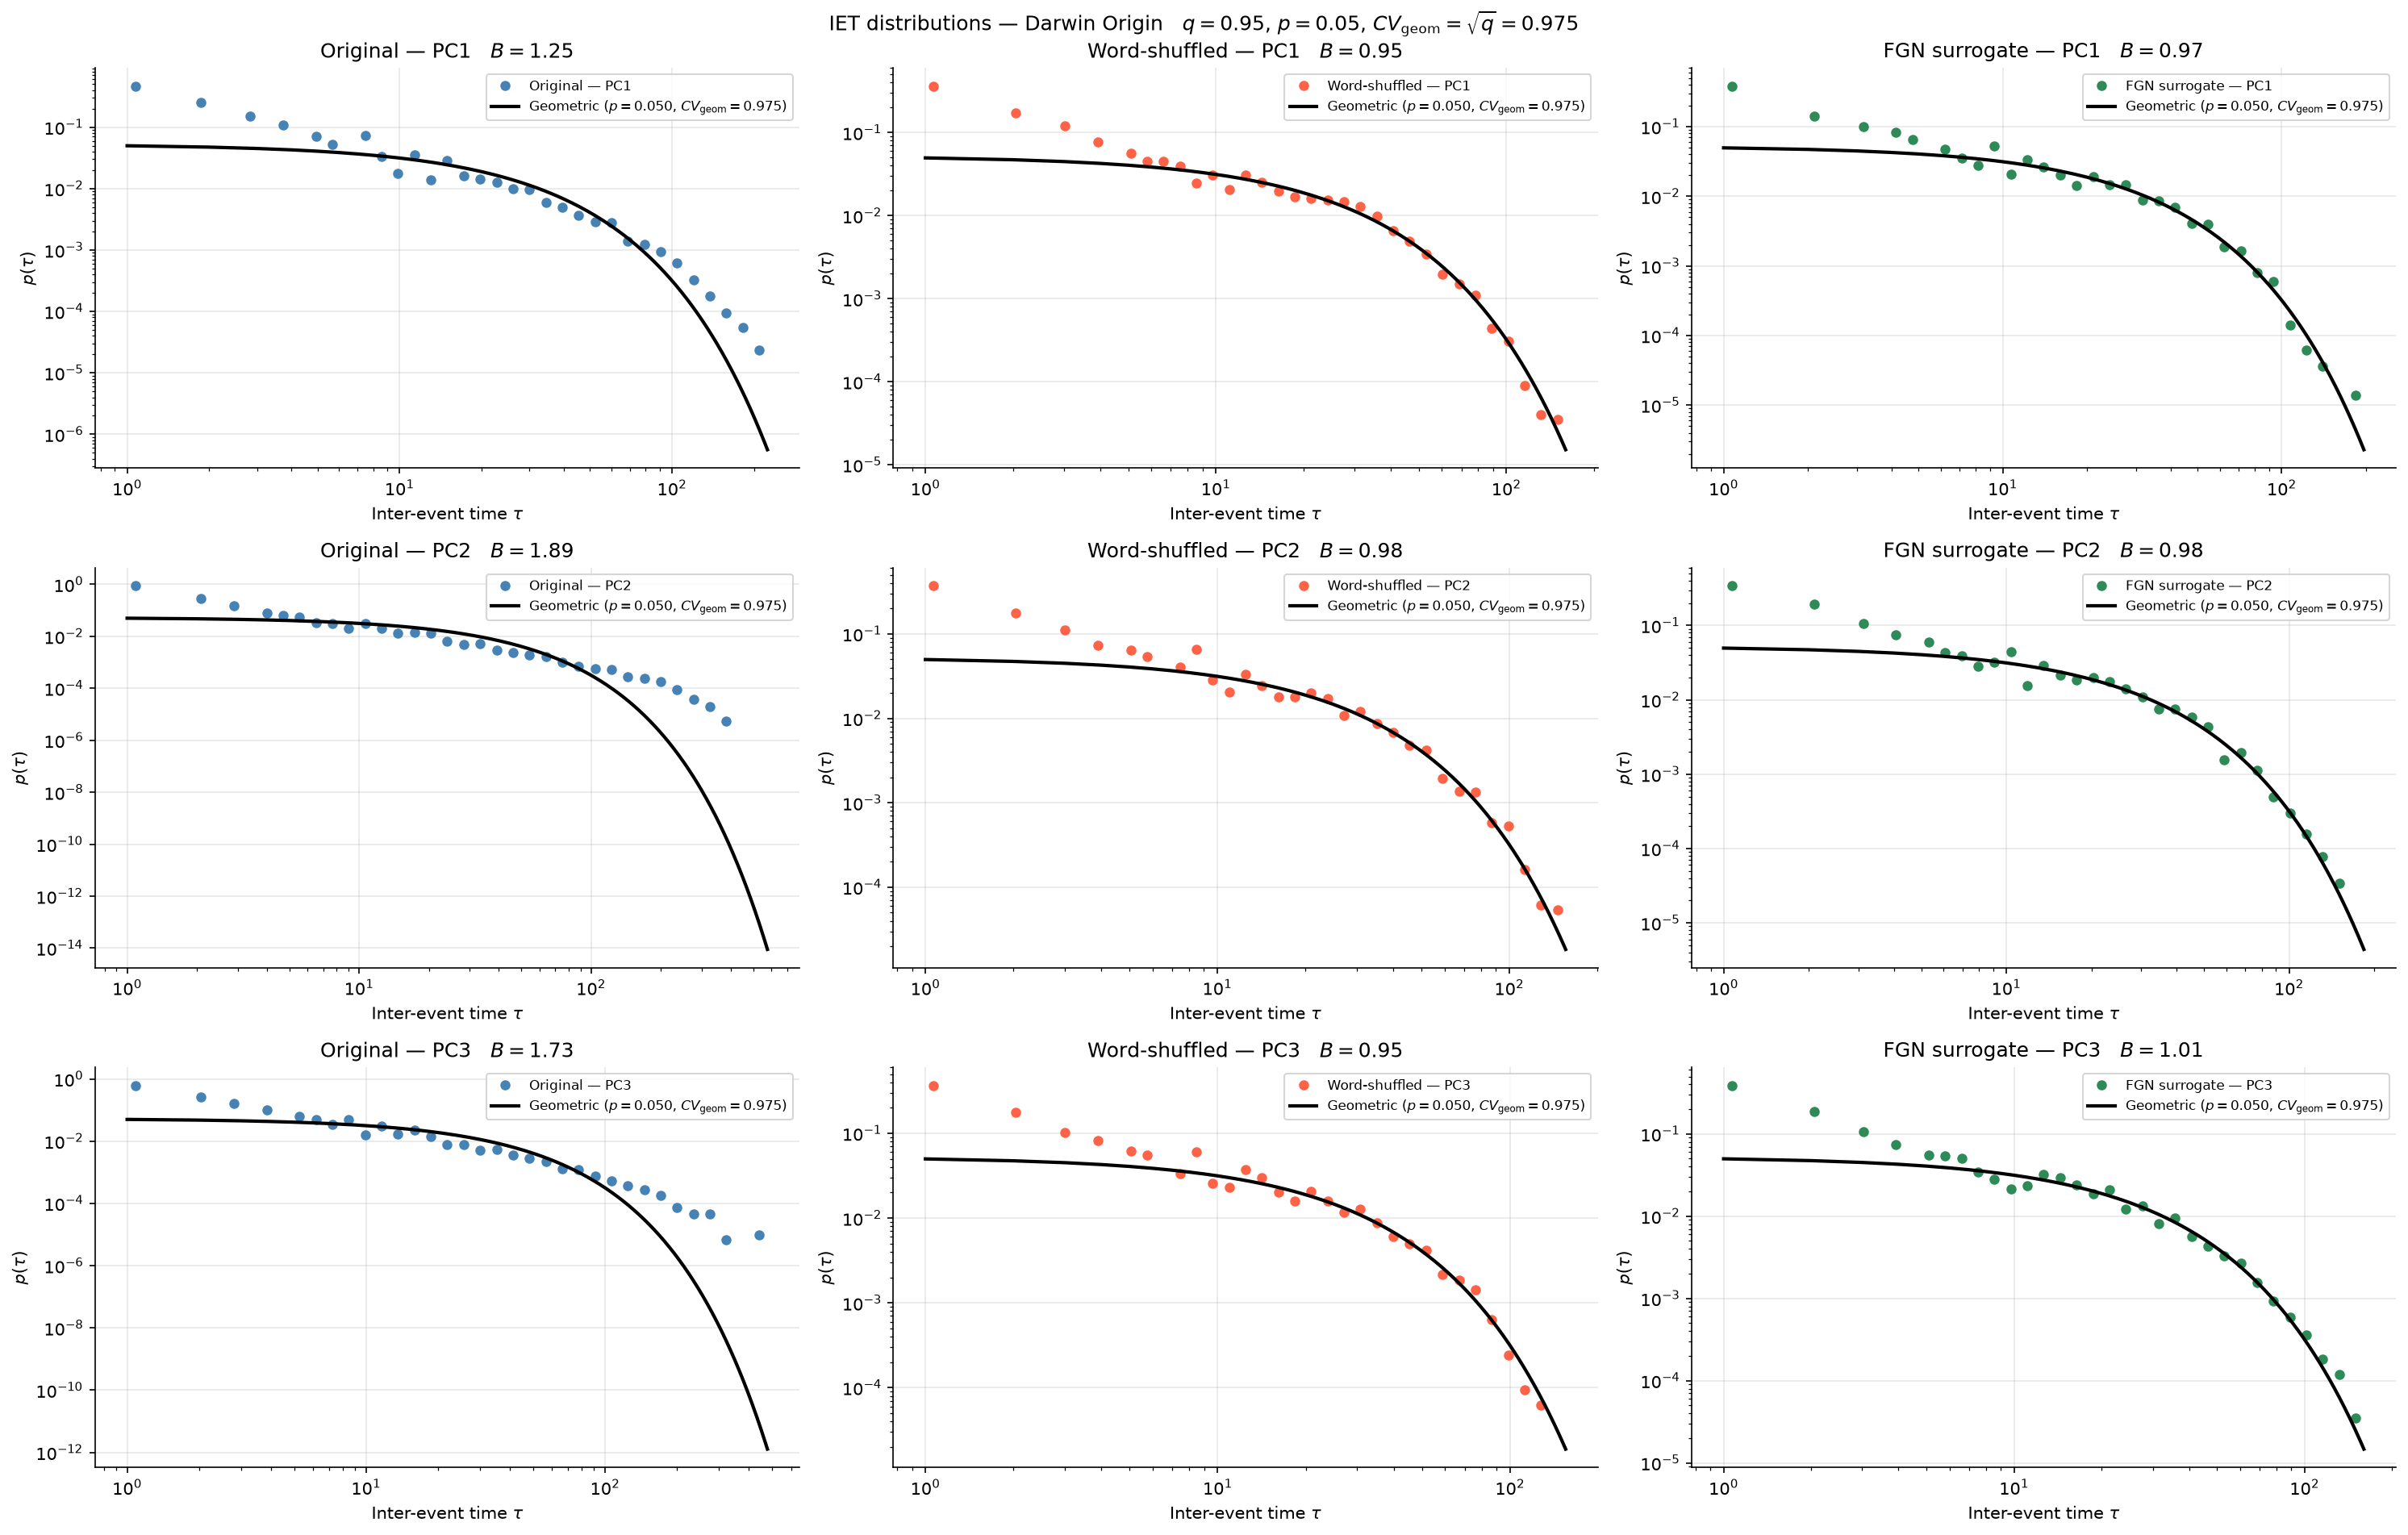
\includegraphics[width=\textwidth]{figures/darwin_origin/darwin_origin_03_iet_comparison.png}
  \caption{Inter-event time distributions for PC1, PC2, PC3 of
  \emph{On the Origin of Species} ($q=0.95$).
  Same conventions as Figure~\ref{fig:wrnpc_iet}.}
  \label{fig:darwin_iet}
\end{figure}

\begin{figure}[htbp]
  \centering
  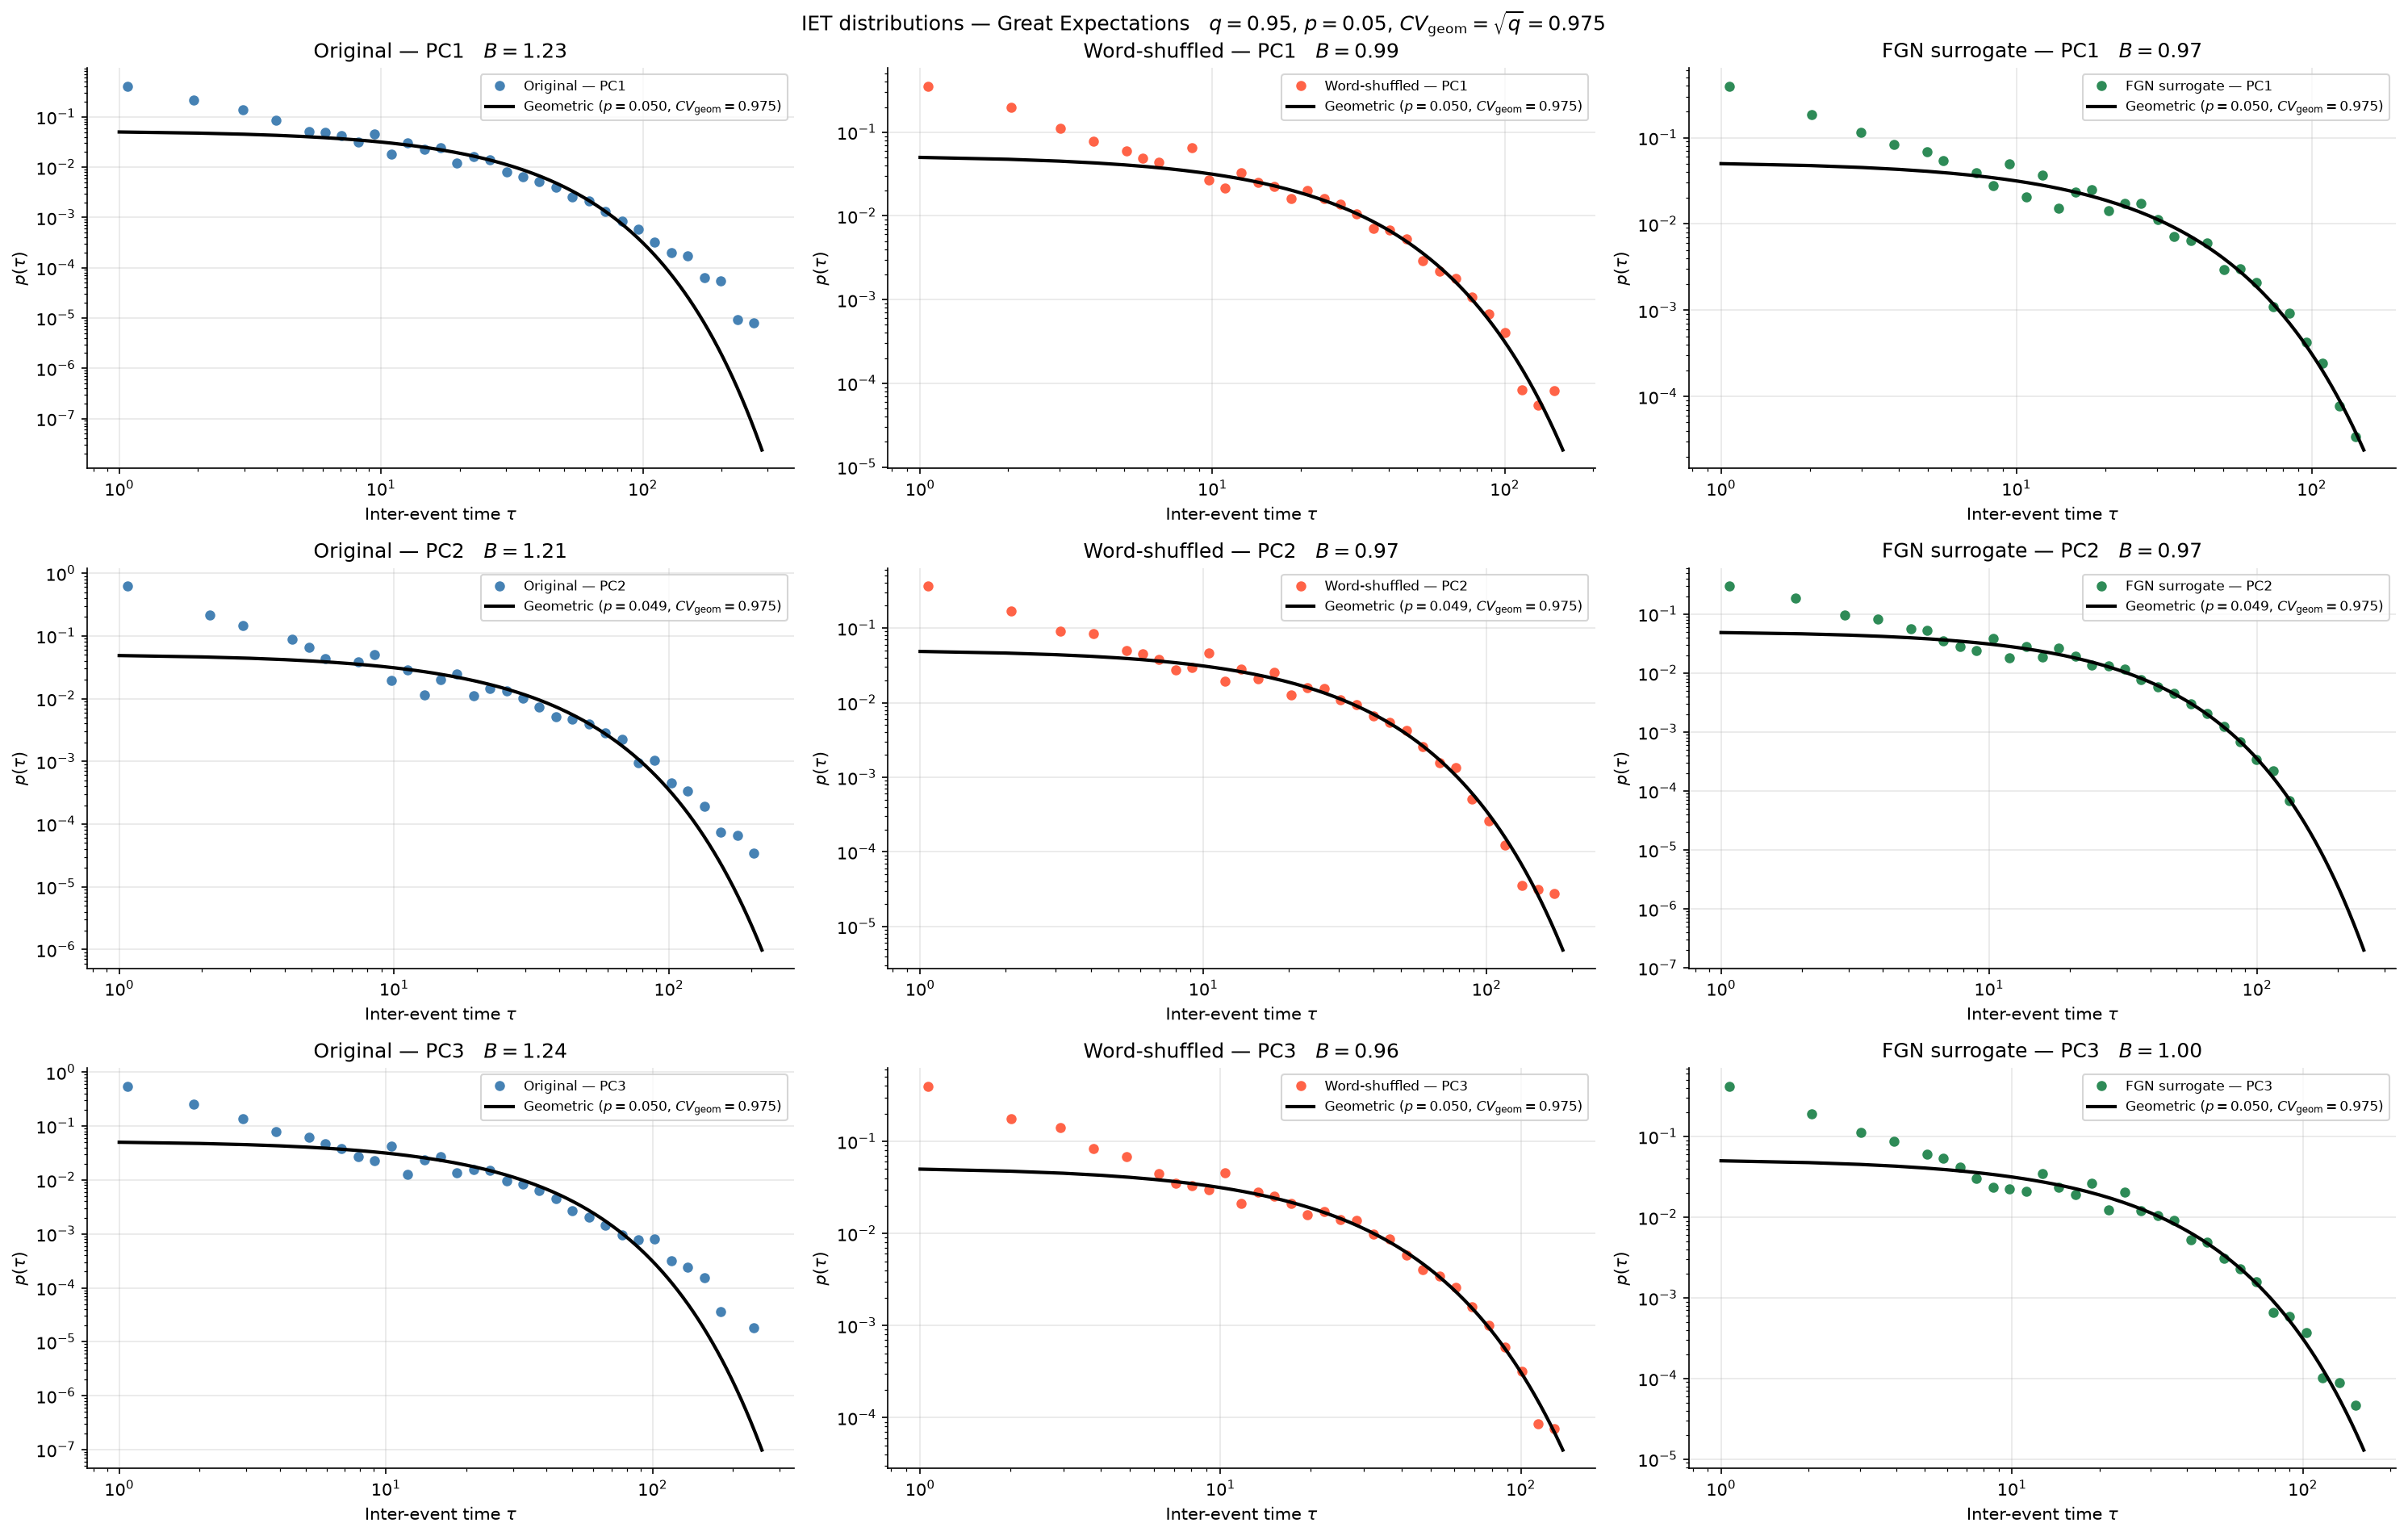
\includegraphics[width=\textwidth]{figures/great_expectations_cut_clean/great_expectations_cut_clean_03_iet_comparison.png}
  \caption{Inter-event time distributions for PC1, PC2, PC3
  of \emph{Great Expectations} ($q=0.95$).
  Same conventions as Figure~\ref{fig:wrnpc_iet}.}
  \label{fig:greatexp_iet}
\end{figure}

\begin{figure}[htbp]
  \centering
  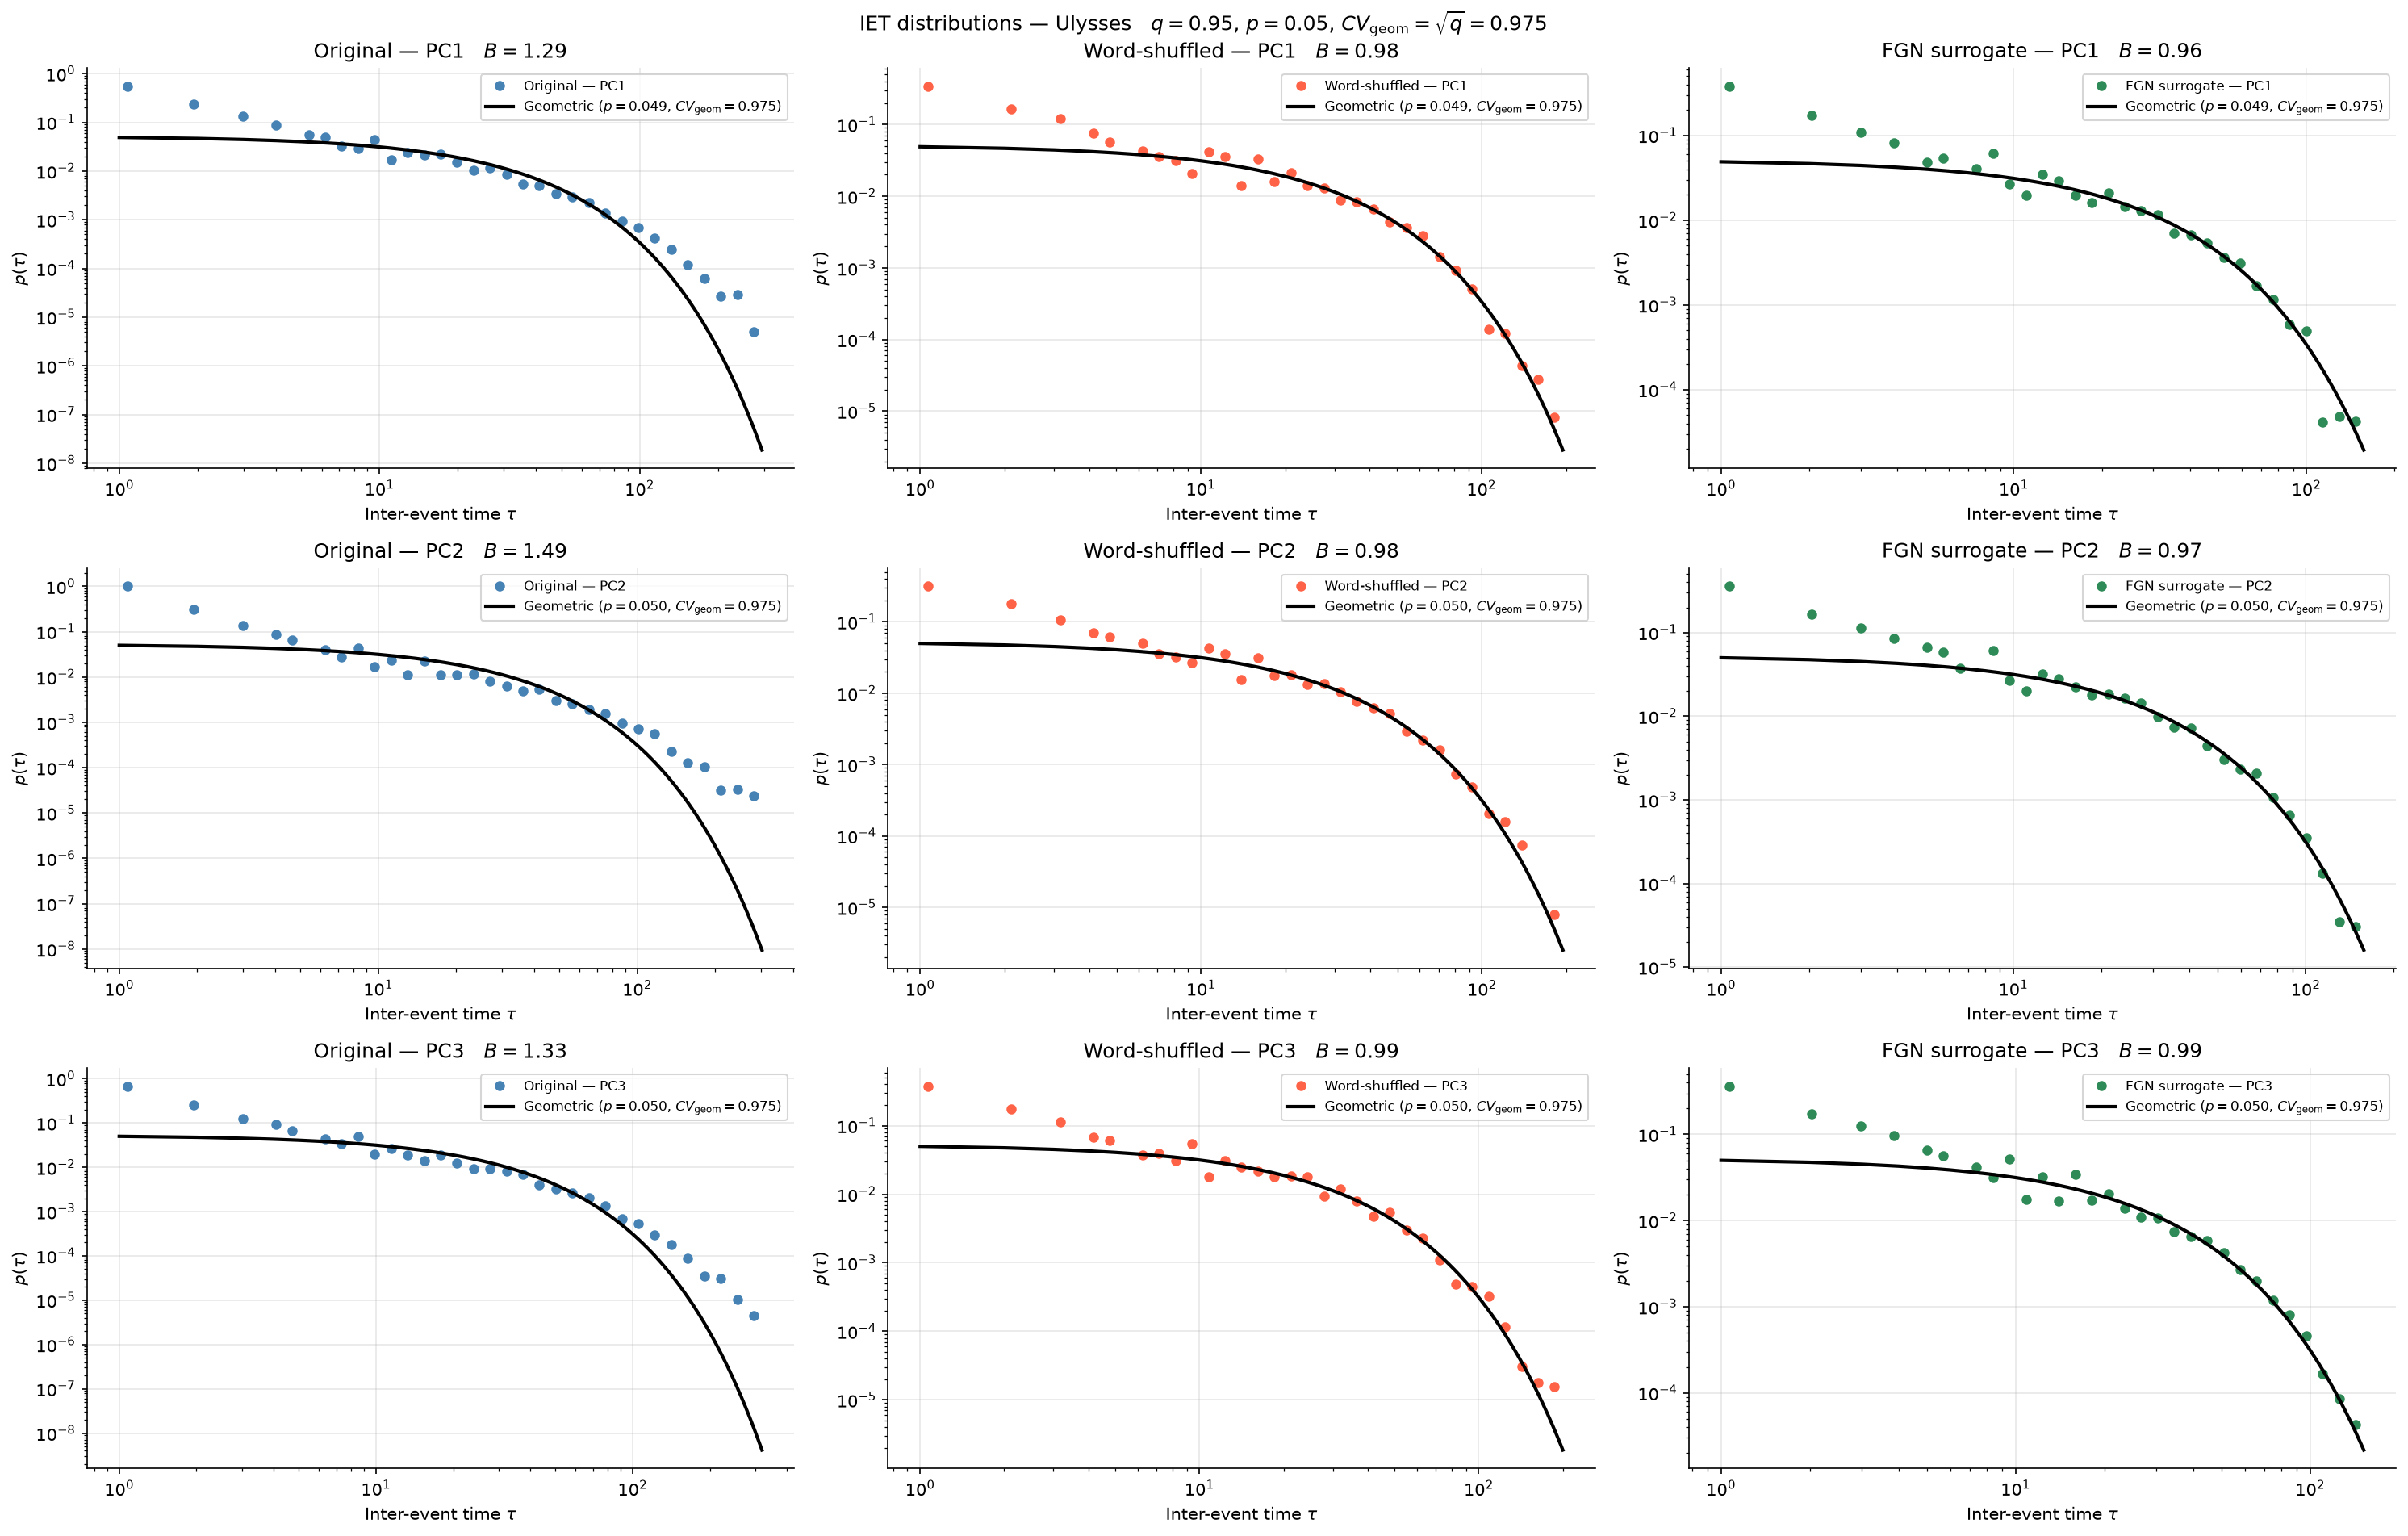
\includegraphics[width=\textwidth]{figures/eng_ulysses/eng_ulysses_03_iet_comparison.png}
  \caption{Inter-event time distributions for PC1, PC2, PC3
  of \emph{Ulysses} ($q=0.95$).
  Same conventions as Figure~\ref{fig:wrnpc_iet}.}
  \label{fig:ulysses_iet}
\end{figure}


%\section{Corpus text list}
%\label{app:corpus}
%
%\NOTE{Table already in Section~\ref{sec:corpus_texts}
%(Table~\ref{tab:corpus}).
%Appendix version to include additional columns:
%OOV rate, $\alpha_0$ (FGN bisection parameter).
%\TODO{Copy and extend from main table.}}


% ──────────────────────────────────────────────────────────
\bibliographystyle{apalike}
\begin{thebibliography}{99}

\bibitem[Alvarez-Lacalle et~al.(2006)]{AlvarezLacalle2006}
Alvarez-Lacalle, E., Dorow, B., Eckmann, J.-P., and Moses, E. (2006).
\newblock Hierarchical structures induce long-range dynamical correlations in written texts.
\newblock \emph{Proceedings of the National Academy of Sciences},
  103(21):7956--7961.

\bibitem[Altmann et~al.(2012)]{Altmann2012}
Altmann, E.~G., Cristadoro, G., and Degli~Esposti, M. (2012).
\newblock On the origin of long-range correlations in texts.
\newblock \emph{Proceedings of the National Academy of Sciences},
  109(29):11582--11587.

\bibitem[Degli~Esposti and Montemurro(2025)]{DegliEsposti2025}
Degli~Esposti, M. and Montemurro, M.~A. (2025).
\newblock A {Z}ipf-preserving, long-range correlated surrogate for
  written language and other symbolic sequences.
\newblock \emph{Physica A: Statistical Mechanics and its Applications}.

\bibitem[Ebeling and Neiman(1995)]{Ebeling1995}
Ebeling, W. and Neiman, A. (1995).
\newblock Long-range correlations between letters and sentences in
  texts.
\newblock \emph{Physica A}, 215:233--241.

\bibitem[Goh and Barab{\'a}si(2008)]{GohBarabasi2008}
Goh, K.-I. and Barab{\'a}si, A.-L. (2008).
\newblock Burstiness and memory in complex systems.
\newblock \emph{Europhysics Letters}, 81:48002.

\bibitem[Mikolov et~al.(2013)]{Mikolov2013}
Mikolov, T., Sutskever, I., Chen, K., Corrado, G.~S., and Dean, J.
  (2013).
\newblock Distributed representations of words and phrases and their
  compositionality.
\newblock In \emph{Advances in Neural Information Processing Systems},
  volume~26.

\bibitem[Montemurro and Degli~Esposti(2025)]{MontemurroDegliEsposti2025}
Montemurro, M.~A. and Degli~Esposti, M. (2025).
\newblock Long-range correlations in {H}eap's law fluctuations.
\newblock \emph{In preparation}.

\bibitem[Montemurro and Pury(2002)]{MontemurroPury2002}
Montemurro, M.~A. and Pury, P.~A. (2002).
\newblock Long-range fractal correlations in literary corpora.
\newblock \emph{Fractals}, 10:451--461.

\bibitem[Peng et~al.(1994)]{Peng1994}
Peng, C.-K., Buldyrev, S.~V., Havlin, S., Simons, M., Stanley,
  H.~E., and Goldberger, A.~L. (1994).
\newblock Mosaic organization of {DNA} nucleotides.
\newblock \emph{Physical Review E}, 49(2):1685--1689.

\bibitem[Pennington et~al.(2014)]{Pennington2014}
Pennington, J., Socher, R., and Manning, C.~D. (2014).
\newblock {G}lo{V}e: Global vectors for word representation.
\newblock In \emph{Proceedings of EMNLP}, pages 1532--1543.

\bibitem[Zipf(1949)]{Zipf1949}
Zipf, G.~K. (1949).
\newblock \emph{Human Behavior and the Principle of Least Effort}.
\newblock Addison-Wesley.

\end{thebibliography}

\end{document}
